\documentclass[a4paper,titlepage,11pt,twosides,floatssmall]{mwrep}
\usepackage[left=2.5cm,right=2.5cm,top=2.5cm,bottom=2.5cm]{geometry}
\usepackage[OT1]{fontenc}
\usepackage{polski}
\usepackage{amsmath}
\usepackage{amsfonts}
\usepackage{amssymb}
\usepackage{graphicx}
\usepackage{url}
\usepackage{tikz}
\usepackage{caption}
\usetikzlibrary{arrows,calc,decorations.markings,math,arrows.meta}
\usepackage{rotating}
\usepackage[percent]{overpic}
\usepackage[utf8x]{inputenc}
\usepackage{xcolor}
\usepackage{pgfplots}
\usetikzlibrary{pgfplots.groupplots}
\usepackage{listings}
\usepackage{matlab-prettifier}
\usepackage{siunitx}
\definecolor{szary}{rgb}{0.95,0.95,0.95}
\sisetup{detect-weight,exponent-product=\cdot,output-decimal-marker={,},per-mode=symbol,binary-units=true,range-phrase={-},range-units=single}

\captionsetup{compatibility=false,justification=centering}


%poprawka kropki/przecinki na wykresach
\SendSettingsToPgf

%konfiguracje pakietu listings
\lstset{
	backgroundcolor=\color{szary},
	frame=single,
	breaklines=true,
    inputencoding=utf8x,
    extendedchars=\true,
    literate={ą}{{\k{a}}}1
             {Ą}{{\k{A}}}1
             {ę}{{\k{e}}}1
             {Ę}{{\k{E}}}1
             {ó}{{\'o}}1
             {Ó}{{\'O}}1
             {ś}{{\'s}}1
             {Ś}{{\'S}}1
             {ł}{{\l{}}}1
             {Ł}{{\L{}}}1
             {ż}{{\.z}}1
             {Ż}{{\.Z}}1
             {ź}{{\'z}}1
             {Ź}{{\'Z}}1
             {ć}{{\'c}}1
             {Ć}{{\'C}}1
             {ń}{{\'n}}1
             {Ń}{{\'N}}1
}
\lstdefinestyle{customlatex}{
	basicstyle=\footnotesize\ttfamily,
	%basicstyle=\small\ttfamily,
}
\lstdefinestyle{customc}{
	breaklines=true,
	frame=tb,
	language=C,
	xleftmargin=0pt,
	showstringspaces=false,
	basicstyle=\small\ttfamily,
	keywordstyle=\bfseries\color{green!40!black},
	commentstyle=\itshape\color{purple!40!black},
	identifierstyle=\color{blue},
	stringstyle=\color{orange},
}
\lstdefinestyle{custommatlab}{
	captionpos=t,
	breaklines=true,
	frame=tb,
	xleftmargin=0pt,
	language=matlab,
	showstringspaces=false,
	%basicstyle=\footnotesize\ttfamily,
	basicstyle=\scriptsize\ttfamily,
	keywordstyle=\bfseries\color{green!40!black},
	commentstyle=\itshape\color{purple!40!black},
	identifierstyle=\color{blue},
	stringstyle=\color{orange},
}

%wymiar tekstu (bez żywej paginy)
\textwidth 160mm \textheight 247mm

%ustawienia pakietu pgfplots
\pgfplotsset{
tick label style={font=\scriptsize},
label style={font=\small},
legend style={font=\small},
title style={font=\small}
}

\def\figurename{Rys.}
\def\tablename{Tab.}

%konfiguracja liczby pływających elementów
\setcounter{topnumber}{0}%2
\setcounter{bottomnumber}{3}%1
\setcounter{totalnumber}{5}%3
\renewcommand{\textfraction}{0.01}%0.2
\renewcommand{\topfraction}{0.95}%0.7
\renewcommand{\bottomfraction}{0.95}%0.3
\renewcommand{\floatpagefraction}{0.35}%0.5

\begin{document}
\frenchspacing
\pagestyle{uheadings}

%strona tytułowa
\title{\bf Sprawozdanie z projektu i ćwiczenia laboratoryjnego nr 1, zadanie nr 5\vskip 0.1cm}
\author{Mateusz Dziwulski, Emilia Gosk, Jakub Szczepański}
\date{2017}

\makeatletter
\renewcommand{\maketitle}{\begin{titlepage}
\begin{center}{\LARGE {\bf
Wydział Elektroniki i Technik Informacyjnych}}\\
\vspace{0.4cm}
{\LARGE {\bf Politechnika Warszawska}}\\
\vspace{0.3cm}
\end{center}
\vspace{5cm}
\begin{center}
{\bf \LARGE Projektowanie układów sterowania\\ (projekt grupowy) \vskip 0.1cm}
\end{center}
\vspace{1cm}
\begin{center}
{\bf \LARGE \@title}
\end{center}
\vspace{2cm}
\begin{center}
{\bf \Large \@author \par}
\end{center}
\vspace*{\stretch{6}}
\begin{center}
\bf{\large{Warszawa, \@date\vskip 0.1cm}}
\end{center}
\end{titlepage}
}
\makeatother

\maketitle

\tableofcontents
\chapter{Wstęp}
Dla prostoty i przejrzystości sprawozdania wykorzystane zostały oznaczenia pierwotnie wprowadzone w skrypcie z przedmiotu STP.

\chapter{Podpunkt 1}
Sprawdzenie poprawności podanych wartości punktu pracy odbywa się poprzez zasymulowanie odpowiedzi procesu w punkcie pracy ($U_{\mathrm{pp}}$, $Y_{\mathrm{pp}}$, $Z_{\mathrm{pp}})$). Z rys. \ref{Z1} widzimy, że podane wartości są poprawne - gdy na wejściu modelu podajemy $U=U_{\mathrm{pp}}=0$ i $Z=Z_{\mathrm{pp}}=\num{0}$, otrzymujemy na wyjściu oczekiwaną przez nas wartość $Y=Y_{\mathrm{pp}}=\num{0}$.

\begin{figure}[ht]
\centering
% This file was created by matlab2tikz.
%
%The latest updates can be retrieved from
%  http://www.mathworks.com/matlabcentral/fileexchange/22022-matlab2tikz-matlab2tikz
%where you can also make suggestions and rate matlab2tikz.
%
\definecolor{mycolor1}{rgb}{0.00000,0.44700,0.74100}%
%
\begin{tikzpicture}

\begin{axis}[%
width=4.521in,
height=3.566in,
at={(0.758in,0.481in)},
scale only axis,
xmin=0,
xmax=250,
xtick={0,50,100,150,200,250},
xlabel style={font=\color{white!15!black}},
xlabel={k},
ymin=25,
ymax=40,
ytick={25,30,35,40},
ylabel style={font=\color{white!15!black}},
ylabel={y},
axis background/.style={fill=white}
]
\addplot [color=mycolor1, forget plot]
  table[row sep=crcr]{%
1	32.68\\
2	32.68\\
3	32.68\\
4	32.68\\
5	32.68\\
6	32.68\\
7	32.68\\
8	32.68\\
9	32.68\\
10	32.68\\
11	32.68\\
12	32.75\\
13	32.75\\
14	32.75\\
15	32.75\\
16	32.75\\
17	32.81\\
18	32.75\\
19	32.81\\
20	32.81\\
21	32.81\\
22	32.81\\
23	32.81\\
24	32.81\\
25	32.81\\
26	32.81\\
27	32.81\\
28	32.81\\
29	32.87\\
30	32.87\\
31	32.81\\
32	32.81\\
33	32.81\\
34	32.81\\
35	32.81\\
36	32.81\\
37	32.81\\
38	32.81\\
39	32.81\\
40	32.81\\
41	32.81\\
42	32.87\\
43	32.87\\
44	32.87\\
45	32.87\\
46	32.87\\
47	32.87\\
48	32.87\\
49	32.87\\
50	32.87\\
51	32.87\\
52	32.87\\
53	32.87\\
54	32.87\\
55	32.87\\
56	32.87\\
57	32.87\\
58	32.87\\
59	32.87\\
60	32.87\\
61	32.87\\
62	32.87\\
63	32.87\\
64	32.87\\
65	32.81\\
66	32.81\\
67	32.81\\
68	32.81\\
69	32.81\\
70	32.81\\
71	32.81\\
72	32.81\\
73	32.81\\
74	32.81\\
75	32.81\\
76	32.81\\
77	32.81\\
78	32.75\\
79	32.81\\
80	32.81\\
81	32.81\\
82	32.75\\
83	32.75\\
84	32.75\\
85	32.75\\
86	32.81\\
87	32.75\\
88	32.81\\
89	32.81\\
90	32.81\\
91	32.81\\
92	32.81\\
93	32.87\\
94	32.93\\
95	33\\
96	33.12\\
97	33.25\\
98	33.37\\
99	33.43\\
100	33.5\\
101	33.5\\
102	33.5\\
103	33.5\\
104	33.5\\
105	33.5\\
106	33.5\\
107	33.43\\
108	33.43\\
109	33.43\\
110	33.43\\
111	33.37\\
112	33.37\\
113	33.37\\
114	33.37\\
115	33.37\\
116	33.31\\
117	33.37\\
118	33.31\\
119	33.31\\
120	33.31\\
121	33.31\\
122	33.31\\
123	33.31\\
124	33.31\\
125	33.31\\
126	33.31\\
127	33.31\\
128	33.25\\
129	33.25\\
130	33.25\\
131	33.25\\
132	33.25\\
133	33.25\\
134	33.25\\
135	33.25\\
136	33.25\\
137	33.18\\
138	33.18\\
139	33.18\\
140	33.18\\
141	33.18\\
142	33.25\\
143	33.18\\
144	33.18\\
145	33.25\\
146	33.18\\
147	33.18\\
148	33.18\\
149	33.18\\
150	33.18\\
151	33.18\\
152	33.18\\
153	33.12\\
154	33.12\\
155	33.12\\
156	33.12\\
157	33.12\\
158	33.12\\
159	33.12\\
160	33.12\\
161	33.12\\
162	33.12\\
163	33.12\\
164	33.12\\
165	33.12\\
166	33.12\\
167	33.12\\
168	33.12\\
169	33.06\\
170	33.12\\
171	33.12\\
172	33.12\\
173	33.12\\
174	33.06\\
175	33.12\\
176	33.12\\
177	33.12\\
178	33.12\\
179	33.12\\
180	33.12\\
181	33.12\\
182	33.12\\
183	33.12\\
184	33.12\\
185	33.12\\
186	33.12\\
187	33.18\\
188	33.18\\
189	33.18\\
190	33.18\\
191	33.12\\
192	33.18\\
193	33.18\\
194	33.12\\
195	33.18\\
196	33.12\\
197	33.12\\
198	33.12\\
199	33.18\\
200	33.12\\
201	33.18\\
202	33.18\\
203	33.18\\
204	33.18\\
205	33.18\\
206	33.18\\
207	33.18\\
208	33.18\\
209	33.18\\
210	33.18\\
211	33.12\\
212	33.12\\
213	33.12\\
214	33.12\\
215	33.12\\
216	33.12\\
217	33.12\\
218	33.12\\
219	33.12\\
220	33.12\\
221	33.12\\
222	33.12\\
223	33.12\\
224	33.12\\
225	33.12\\
226	33.12\\
227	33.12\\
228	33.12\\
229	33.06\\
230	33.06\\
231	33.06\\
232	33.06\\
233	33.06\\
234	33.06\\
235	33.06\\
236	33.06\\
237	33\\
238	33\\
239	33\\
240	33\\
241	33\\
242	33\\
243	33\\
244	33\\
245	33.06\\
246	33.06\\
247	33.06\\
248	33.06\\
249	33.06\\
250	33.06\\
};
\end{axis}
\end{tikzpicture}%
\caption{Sprawdzenie poprawności punktu pracy}
\label{Z1}
\end{figure}


\chapter{Podpunkt 2}
Dla reprezentacji odpowiedzi skokowych wybranych zostało sześć różnych wartości zmian sygnału sterującego i sygnału zakłóceń: od $U_{\mathrm{pp}}$ do kilku $U_{\mathrm{s}}$ oraz od $Z_{\mathrm{pp}}$ do  $Z_{\mathrm{s}}$, skok w obu torach wystąpił w chwili $k=10$. Wykresy odpowiedzi skokowych zamieszczone zostały na rysunkach \ref{Z2a} i \ref{Z2b}.

\begin{figure}[ht]
\centering

\definecolor{mycolor1}{rgb}{0.00000,0.44700,0.74100}%
\definecolor{mycolor2}{rgb}{0.85000,0.32500,0.09800}%
\definecolor{mycolor3}{rgb}{0.92900,0.69400,0.12500}%
\definecolor{mycolor4}{rgb}{0.49400,0.18400,0.55600}%
\definecolor{mycolor5}{rgb}{0.46600,0.67400,0.18800}%
\definecolor{mycolor6}{rgb}{0.30100,0.74500,0.93300}%
%
\begin{tikzpicture}

\begin{axis}[%
width=4.667in,
height=0.645in,
at={(0.583in,0.52in)},
scale only axis,
xmin=0,
xmax=200,
xtick={0,20,40,60,80,100,120,140,160,180,200},
xlabel style={font=\color{white!15!black}},
xlabel={$k$},
ymin=-0.5,
ymax=0.5,
ytick={-0.5,0,0.5},
ylabel style={font=\color{white!15!black}},
ylabel={$u$},
axis background/.style={fill=white}
]
\addplot[const plot, color=mycolor1, forget plot] table[row sep=crcr] {%
1	0\\
10	0.5\\
200	0.5\\
};
\addplot[const plot, color=mycolor2, forget plot] table[row sep=crcr] {%
1	0\\
10	0.300000000000011\\
200	0.300000000000011\\
};
\addplot[const plot, color=mycolor3, forget plot] table[row sep=crcr] {%
1	0\\
10	0.0999999999999943\\
200	0.0999999999999943\\
};
\addplot[const plot, color=mycolor4, forget plot] table[row sep=crcr] {%
1	0\\
10	-0.0999999999999943\\
200	-0.0999999999999943\\
};
\addplot[const plot, color=mycolor5, forget plot] table[row sep=crcr] {%
1	0\\
10	-0.300000000000011\\
200	-0.300000000000011\\
};
\addplot[const plot, color=mycolor6, forget plot] table[row sep=crcr] {%
1	0\\
10	-0.5\\
200	-0.5\\
};
\end{axis}

\begin{axis}[%
width=4.667in,
height=0.645in,
at={(0.583in,1.613in)},
scale only axis,
xmin=0,
xmax=200,
xtick={0,20,40,60,80,100,120,140,160,180,200},
ymin=-1,
ymax=1,
ytick={-1,0,1},
ylabel style={font=\color{white!15!black}},
ylabel={$z$},
axis background/.style={fill=white}
]
\addplot[const plot, color=mycolor1, forget plot] table[row sep=crcr] {%
1	0\\
200	0\\
};
\addplot[const plot, color=mycolor2, forget plot] table[row sep=crcr] {%
1	0\\
200	0\\
};
\addplot[const plot, color=mycolor3, forget plot] table[row sep=crcr] {%
1	0\\
200	0\\
};
\addplot[const plot, color=mycolor4, forget plot] table[row sep=crcr] {%
1	0\\
200	0\\
};
\addplot[const plot, color=mycolor5, forget plot] table[row sep=crcr] {%
1	0\\
200	0\\
};
\addplot[const plot, color=mycolor6, forget plot] table[row sep=crcr] {%
1	0\\
200	0\\
};
\end{axis}

\begin{axis}[%
width=4.667in,
height=2.625in,
at={(0.583in,2.707in)},
scale only axis,
xmin=0,
xmax=200,
xtick={0,20,40,60,80,100,120,140,160,180,200},
ymin=-0.8,
ymax=0.8,
ytick={-0.8,-0.6,-0.4,-0.2,0,0.2,0.4,0.6,0.8},
ylabel style={font=\color{white!15!black}},
ylabel={$y$},
axis background/.style={fill=white},
legend style={legend cell align=left, align=left, draw=white!15!black}
]
\addplot [color=mycolor1]
  table[row sep=crcr]{%
1	0\\
14	0\\
15	0.0384530000000041\\
16	0.0749336336000113\\
17	0.109542195598323\\
18	0.142373983848046\\
19	0.173519535957837\\
20	0.203064856269236\\
21	0.231091633319494\\
22	0.257677448023259\\
23	0.282895972823468\\
24	0.30681716207684\\
25	0.329507433948635\\
26	0.351029844097951\\
27	0.371444251438646\\
28	0.390807476263433\\
29	0.409173451016613\\
30	0.426593364000041\\
31	0.443115796293228\\
32	0.458786852163144\\
33	0.473650283234605\\
34	0.487747606685645\\
35	0.501118217724581\\
36	0.513799496599688\\
37	0.525826910383444\\
38	0.537234109766075\\
39	0.548053021085082\\
40	0.558313933809387\\
41	0.568045583688246\\
43	0.586028739470578\\
45	0.602204205701184\\
47	0.616753503760123\\
49	0.629839969252799\\
51	0.641610564692229\\
53	0.652197513553432\\
55	0.661719772844975\\
57	0.67028435980103\\
59	0.677987546868934\\
61	0.684915937851457\\
64	0.694024034572209\\
67	0.701793023605148\\
70	0.708419743854677\\
73	0.714072113436544\\
76	0.718893374820226\\
80	0.724237441423838\\
84	0.728560337646286\\
89	0.732821530148641\\
94	0.736090465036796\\
100	0.739024784995109\\
107	0.741453905054584\\
116	0.743505122649907\\
127	0.744987403130921\\
143	0.746057979161634\\
169	0.746657552697201\\
200	0.74682046969906\\
};
\addlegendentry{$\text{U}_\text{s}\text{=0,5}$}

\addplot [color=mycolor2]
  table[row sep=crcr]{%
1	0\\
14	0\\
15	0.0230717999999968\\
16	0.0449601801599897\\
17	0.0657253173589822\\
18	0.0854243903088161\\
19	0.104111721574697\\
20	0.121838913761536\\
21	0.138654979991713\\
22	0.154606468813967\\
23	0.169737583694086\\
24	0.184090297246087\\
25	0.197704460369181\\
26	0.210617906458765\\
27	0.222866550863188\\
28	0.23448448575806\\
29	0.245504070609968\\
30	0.255956018400042\\
31	0.265869477775937\\
33	0.284190169940786\\
35	0.300670930634737\\
37	0.315496146230061\\
39	0.32883181265106\\
41	0.340827350212948\\
43	0.351617243682341\\
45	0.361322523420711\\
47	0.370052102256068\\
49	0.377903981551668\\
51	0.384966338815332\\
53	0.391318508132059\\
56	0.399669311800608\\
59	0.406792528121343\\
62	0.41286854712402\\
65	0.418051272360316\\
69	0.423796106942746\\
73	0.428443268061926\\
77	0.43220246100978\\
82	0.43590802393993\\
88	0.439234308946425\\
95	0.441987929706329\\
103	0.444106132822327\\
113	0.445756088987139\\
127	0.446992441878535\\
148	0.447746776318183\\
190	0.448075904878323\\
200	0.448092281819413\\
};
\addlegendentry{$\text{U}_\text{s}\text{=0,3}$}

\addplot [color=mycolor3]
  table[row sep=crcr]{%
1	0\\
14	0\\
16	0.0149867267199966\\
18	0.0284747967696148\\
20	0.0406129712538359\\
22	0.051535489604646\\
24	0.0613634324153622\\
26	0.0702059688195789\\
28	0.0781614952526866\\
30	0.0853186728000139\\
32	0.0917573704326173\\
35	0.100223643544922\\
38	0.107446821953204\\
41	0.113609116737649\\
44	0.118866127984148\\
48	0.124694008330692\\
52	0.129408853084527\\
56	0.133223103933545\\
61	0.13698318757028\\
67	0.14035860472103\\
74	0.143153022090615\\
82	0.145302674646643\\
92	0.146977162854739\\
106	0.1482319148503\\
127	0.148997480626178\\
169	0.14933151053944\\
200	0.149364093939795\\
};
\addlegendentry{$\text{U}_\text{s}\text{=0,1}$}

\addplot [color=mycolor4]
  table[row sep=crcr]{%
1	0\\
14	0\\
16	-0.0149867267199966\\
18	-0.0284747967696148\\
20	-0.0406129712538359\\
22	-0.051535489604646\\
24	-0.0613634324153622\\
26	-0.0702059688195789\\
28	-0.0781614952526866\\
30	-0.0853186728000139\\
32	-0.0917573704326173\\
35	-0.100223643544922\\
38	-0.107446821953204\\
41	-0.113609116737649\\
44	-0.118866127984148\\
48	-0.124694008330692\\
52	-0.129408853084527\\
56	-0.133223103933545\\
61	-0.13698318757028\\
67	-0.14035860472103\\
74	-0.143153022090615\\
82	-0.145302674646643\\
92	-0.146977162854739\\
106	-0.1482319148503\\
127	-0.148997480626178\\
169	-0.14933151053944\\
200	-0.149364093939795\\
};
\addlegendentry{$\text{U}_\text{s}\text{=-0,1}$}

\addplot [color=mycolor5]
  table[row sep=crcr]{%
1	0\\
14	0\\
15	-0.0230717999999968\\
16	-0.0449601801599897\\
17	-0.0657253173589822\\
18	-0.0854243903088161\\
19	-0.104111721574697\\
20	-0.121838913761536\\
21	-0.138654979991713\\
22	-0.154606468813967\\
23	-0.169737583694086\\
24	-0.184090297246087\\
25	-0.197704460369181\\
26	-0.210617906458765\\
27	-0.222866550863188\\
28	-0.23448448575806\\
29	-0.245504070609968\\
30	-0.255956018400042\\
31	-0.265869477775937\\
33	-0.284190169940786\\
35	-0.300670930634737\\
37	-0.315496146230061\\
39	-0.32883181265106\\
41	-0.340827350212948\\
43	-0.351617243682341\\
45	-0.361322523420711\\
47	-0.370052102256068\\
49	-0.377903981551668\\
51	-0.384966338815332\\
53	-0.391318508132059\\
56	-0.399669311800608\\
59	-0.406792528121343\\
62	-0.41286854712402\\
65	-0.418051272360316\\
69	-0.423796106942746\\
73	-0.428443268061926\\
77	-0.43220246100978\\
82	-0.43590802393993\\
88	-0.439234308946425\\
95	-0.441987929706329\\
103	-0.444106132822327\\
113	-0.445756088987139\\
127	-0.446992441878535\\
148	-0.447746776318183\\
190	-0.448075904878323\\
200	-0.448092281819413\\
};
\addlegendentry{$\text{U}_\text{s}\text{=-0,3}$}

\addplot [color=mycolor6]
  table[row sep=crcr]{%
1	0\\
14	0\\
15	-0.0384530000000041\\
16	-0.0749336336000113\\
17	-0.109542195598323\\
18	-0.142373983848046\\
19	-0.173519535957837\\
20	-0.203064856269236\\
21	-0.231091633319494\\
22	-0.257677448023259\\
23	-0.282895972823468\\
24	-0.30681716207684\\
25	-0.329507433948635\\
26	-0.351029844097951\\
27	-0.371444251438646\\
28	-0.390807476263433\\
29	-0.409173451016613\\
30	-0.426593364000041\\
31	-0.443115796293228\\
32	-0.458786852163144\\
33	-0.473650283234605\\
34	-0.487747606685645\\
35	-0.501118217724581\\
36	-0.513799496599688\\
37	-0.525826910383444\\
38	-0.537234109766075\\
39	-0.548053021085082\\
40	-0.558313933809387\\
41	-0.568045583688246\\
43	-0.586028739470578\\
45	-0.602204205701184\\
47	-0.616753503760123\\
49	-0.629839969252799\\
51	-0.641610564692229\\
53	-0.652197513553432\\
55	-0.661719772844975\\
57	-0.67028435980103\\
59	-0.677987546868934\\
61	-0.684915937851457\\
64	-0.694024034572209\\
67	-0.701793023605148\\
70	-0.708419743854677\\
73	-0.714072113436544\\
76	-0.718893374820226\\
80	-0.724237441423838\\
84	-0.728560337646286\\
89	-0.732821530148641\\
94	-0.736090465036796\\
100	-0.739024784995109\\
107	-0.741453905054584\\
116	-0.743505122649907\\
127	-0.744987403130921\\
143	-0.746057979161634\\
169	-0.746657552697201\\
200	-0.74682046969906\\
};
\addlegendentry{$\text{U}_\text{s}\text{=-0,5}$}

\end{axis}
\end{tikzpicture}%
\caption{Odpowiedzi dla skoków sygnału sterującego} 
\label{Z2a}
\end{figure}

\begin{figure}[ht]
\centering

\definecolor{mycolor1}{rgb}{0.00000,0.44700,0.74100}%
\definecolor{mycolor2}{rgb}{0.85000,0.32500,0.09800}%
\definecolor{mycolor3}{rgb}{0.92900,0.69400,0.12500}%
\definecolor{mycolor4}{rgb}{0.49400,0.18400,0.55600}%
\definecolor{mycolor5}{rgb}{0.46600,0.67400,0.18800}%
\definecolor{mycolor6}{rgb}{0.30100,0.74500,0.93300}%
%
\begin{tikzpicture}

\begin{axis}[%
width=4.667in,
height=0.645in,
at={(0.583in,0.52in)},
scale only axis,
xmin=0,
xmax=200,
xtick={0,20,40,60,80,100,120,140,160,180,200},
xlabel style={font=\color{white!15!black}},
xlabel={$k$},
ymin=-1,
ymax=1,
ytick={-1,0,1},
ylabel style={font=\color{white!15!black}},
ylabel={$u$},
axis background/.style={fill=white}
]
\addplot[const plot, color=mycolor1, forget plot] table[row sep=crcr] {%
1	0\\
200	0\\
};
\addplot[const plot, color=mycolor2, forget plot] table[row sep=crcr] {%
1	0\\
200	0\\
};
\addplot[const plot, color=mycolor3, forget plot] table[row sep=crcr] {%
1	0\\
200	0\\
};
\addplot[const plot, color=mycolor4, forget plot] table[row sep=crcr] {%
1	0\\
200	0\\
};
\addplot[const plot, color=mycolor5, forget plot] table[row sep=crcr] {%
1	0\\
200	0\\
};
\addplot[const plot, color=mycolor6, forget plot] table[row sep=crcr] {%
1	0\\
200	0\\
};
\end{axis}

\begin{axis}[%
width=4.667in,
height=0.645in,
at={(0.583in,1.613in)},
scale only axis,
xmin=0,
xmax=200,
xtick={0,20,40,60,80,100,120,140,160,180,200},
ymin=-0.5,
ymax=0.5,
ytick={-0.5,0,0.5},
ylabel style={font=\color{white!15!black}},
ylabel={$z$},
axis background/.style={fill=white}
]
\addplot[const plot, color=mycolor1, forget plot] table[row sep=crcr] {%
1	0\\
10	0.5\\
200	0.5\\
};
\addplot[const plot, color=mycolor2, forget plot] table[row sep=crcr] {%
1	0\\
10	0.300000000000011\\
200	0.300000000000011\\
};
\addplot[const plot, color=mycolor3, forget plot] table[row sep=crcr] {%
1	0\\
10	0.0999999999999943\\
200	0.0999999999999943\\
};
\addplot[const plot, color=mycolor4, forget plot] table[row sep=crcr] {%
1	0\\
10	-0.0999999999999943\\
200	-0.0999999999999943\\
};
\addplot[const plot, color=mycolor5, forget plot] table[row sep=crcr] {%
1	0\\
10	-0.300000000000011\\
200	-0.300000000000011\\
};
\addplot[const plot, color=mycolor6, forget plot] table[row sep=crcr] {%
1	0\\
10	-0.5\\
200	-0.5\\
};
\end{axis}

\begin{axis}[%
width=4.667in,
height=2.625in,
at={(0.583in,2.707in)},
scale only axis,
xmin=0,
xmax=200,
xtick={0,20,40,60,80,100,120,140,160,180,200},
ymin=-0.5,
ymax=0.5,
ytick={-0.5,0,0.5},
ylabel style={font=\color{white!15!black}},
ylabel={$y$},
axis background/.style={fill=white},
legend style={legend cell align=left, align=left, draw=white!15!black}
]
\addplot [color=mycolor1]
  table[row sep=crcr]{%
1	0\\
12	0\\
13	0.0528750000000002\\
14	0.0995346999999924\\
15	0.140708348890001\\
16	0.17703970091236\\
17	0.209097035202575\\
18	0.237382001274085\\
19	0.262337428009744\\
20	0.284354217604715\\
21	0.303777431676593\\
22	0.320911664196615\\
23	0.336025784805628\\
24	0.349357126287458\\
25	0.361115181329069\\
26	0.371484866065629\\
27	0.380629401171603\\
28	0.388692855312001\\
29	0.395802390516394\\
30	0.40207024440366\\
31	0.407595480092141\\
32	0.412465531017745\\
33	0.416757564692574\\
34	0.420539686620401\\
35	0.423872003100456\\
36	0.426807559454602\\
37	0.429393168277414\\
39	0.433674931319558\\
41	0.436992858906791\\
43	0.439561511336535\\
45	0.44154792221326\\
48	0.443712164043603\\
51	0.445176001257778\\
55	0.446411781079149\\
60	0.447259620735963\\
67	0.447780419566584\\
80	0.448002533908351\\
169	0.447935342164698\\
200	0.447934166332374\\
};
\addlegendentry{$\text{Z}_\text{s}\text{=0,5}$}

\addplot [color=mycolor2]
  table[row sep=crcr]{%
1	0\\
12	0\\
13	0.0317249999999945\\
14	0.0597208199999955\\
15	0.0844250093340122\\
16	0.106223820547427\\
17	0.125458221121534\\
18	0.14242920076444\\
19	0.157402456805841\\
20	0.170612530562835\\
21	0.182266459005945\\
22	0.192546998517969\\
23	0.201615470883382\\
24	0.209614275772481\\
25	0.216669108797447\\
26	0.222890919639383\\
27	0.228377640702973\\
28	0.233215713187207\\
29	0.237481434309842\\
30	0.241242146642207\\
31	0.24455728805529\\
32	0.247479318610658\\
33	0.250054538815533\\
35	0.254323201860274\\
37	0.257635900966449\\
39	0.260204958791746\\
41	0.262195715344092\\
44	0.264371165655234\\
47	0.26584926141399\\
51	0.267105600754661\\
56	0.2679782586942\\
63	0.26852865044026\\
76	0.268787928491719\\
135	0.268765581528669\\
200	0.268760499799413\\
};
\addlegendentry{$\text{Z}_\text{s}\text{=0,3}$}

\addplot [color=mycolor3]
  table[row sep=crcr]{%
1	0\\
12	0\\
13	0.0105749999999887\\
14	0.0199069399999985\\
15	0.0281416697779946\\
16	0.0354079401824663\\
17	0.0418194070405207\\
18	0.0474764002548227\\
19	0.0524674856019374\\
20	0.0568708435209544\\
21	0.0607554863353243\\
22	0.064182332839323\\
23	0.0672051569611369\\
24	0.069871425257503\\
26	0.0742969732131371\\
28	0.0777385710624117\\
30	0.0804140488807263\\
32	0.0824931062035432\\
35	0.0847744006200912\\
38	0.0863340281192393\\
42	0.0876718853709235\\
47	0.0886164204713396\\
54	0.0892323254356882\\
66	0.08954691314716\\
104	0.0895949830109544\\
200	0.0895868332664804\\
};
\addlegendentry{$\text{Z}_\text{s}\text{=0,1}$}

\addplot [color=mycolor4]
  table[row sep=crcr]{%
1	0\\
12	0\\
13	-0.0105749999999887\\
14	-0.0199069399999985\\
15	-0.0281416697779946\\
16	-0.0354079401824663\\
17	-0.0418194070405207\\
18	-0.0474764002548227\\
19	-0.0524674856019374\\
20	-0.0568708435209544\\
21	-0.0607554863353243\\
22	-0.064182332839323\\
23	-0.0672051569611369\\
24	-0.069871425257503\\
26	-0.0742969732131371\\
28	-0.0777385710624117\\
30	-0.0804140488807263\\
32	-0.0824931062035432\\
35	-0.0847744006200912\\
38	-0.0863340281192393\\
42	-0.0876718853709235\\
47	-0.0886164204713396\\
54	-0.0892323254356882\\
66	-0.08954691314716\\
104	-0.0895949830109544\\
200	-0.0895868332664804\\
};
\addlegendentry{$\text{Z}_\text{s}\text{=-0,1}$}

\addplot [color=mycolor5]
  table[row sep=crcr]{%
1	0\\
12	0\\
13	-0.0317249999999945\\
14	-0.0597208199999955\\
15	-0.0844250093340122\\
16	-0.106223820547427\\
17	-0.125458221121534\\
18	-0.14242920076444\\
19	-0.157402456805841\\
20	-0.170612530562835\\
21	-0.182266459005945\\
22	-0.192546998517969\\
23	-0.201615470883382\\
24	-0.209614275772481\\
25	-0.216669108797447\\
26	-0.222890919639383\\
27	-0.228377640702973\\
28	-0.233215713187207\\
29	-0.237481434309842\\
30	-0.241242146642207\\
31	-0.24455728805529\\
32	-0.247479318610658\\
33	-0.250054538815533\\
35	-0.254323201860274\\
37	-0.257635900966449\\
39	-0.260204958791746\\
41	-0.262195715344092\\
44	-0.264371165655234\\
47	-0.26584926141399\\
51	-0.267105600754661\\
56	-0.2679782586942\\
63	-0.26852865044026\\
76	-0.268787928491719\\
135	-0.268765581528669\\
200	-0.268760499799413\\
};
\addlegendentry{$\text{Z}_\text{s}\text{=-0,3}$}

\addplot [color=mycolor6]
  table[row sep=crcr]{%
1	0\\
12	0\\
13	-0.0528750000000002\\
14	-0.0995346999999924\\
15	-0.140708348890001\\
16	-0.17703970091236\\
17	-0.209097035202575\\
18	-0.237382001274085\\
19	-0.262337428009744\\
20	-0.284354217604715\\
21	-0.303777431676593\\
22	-0.320911664196615\\
23	-0.336025784805628\\
24	-0.349357126287458\\
25	-0.361115181329069\\
26	-0.371484866065629\\
27	-0.380629401171603\\
28	-0.388692855312001\\
29	-0.395802390516394\\
30	-0.40207024440366\\
31	-0.407595480092141\\
32	-0.412465531017745\\
33	-0.416757564692574\\
34	-0.420539686620401\\
35	-0.423872003100456\\
36	-0.426807559454602\\
37	-0.429393168277414\\
39	-0.433674931319558\\
41	-0.436992858906791\\
43	-0.439561511336535\\
45	-0.44154792221326\\
48	-0.443712164043603\\
51	-0.445176001257778\\
55	-0.446411781079149\\
60	-0.447259620735963\\
67	-0.447780419566584\\
80	-0.448002533908351\\
169	-0.447935342164698\\
200	-0.447934166332374\\
};
\addlegendentry{$\text{Z}_\text{s}\text{=-0,5}$}

\end{axis}
\end{tikzpicture}%
\caption{Odpowiedzi dla skoków sygnału zakłóceń}
\label{Z2b}
\end{figure}

Symulując odpowiedź układu dla różnych wartości sygnału sterującego i zakłócającego otrzymujemy charakterystykę statyczną $y(u,z)$ widoczną na rys. \ref{Z2c} (ze względów estetycznych dodane zostało kolorowanie, nie reprezentuje ono żadnej wartości).

\begin{figure}[ht]
\centering

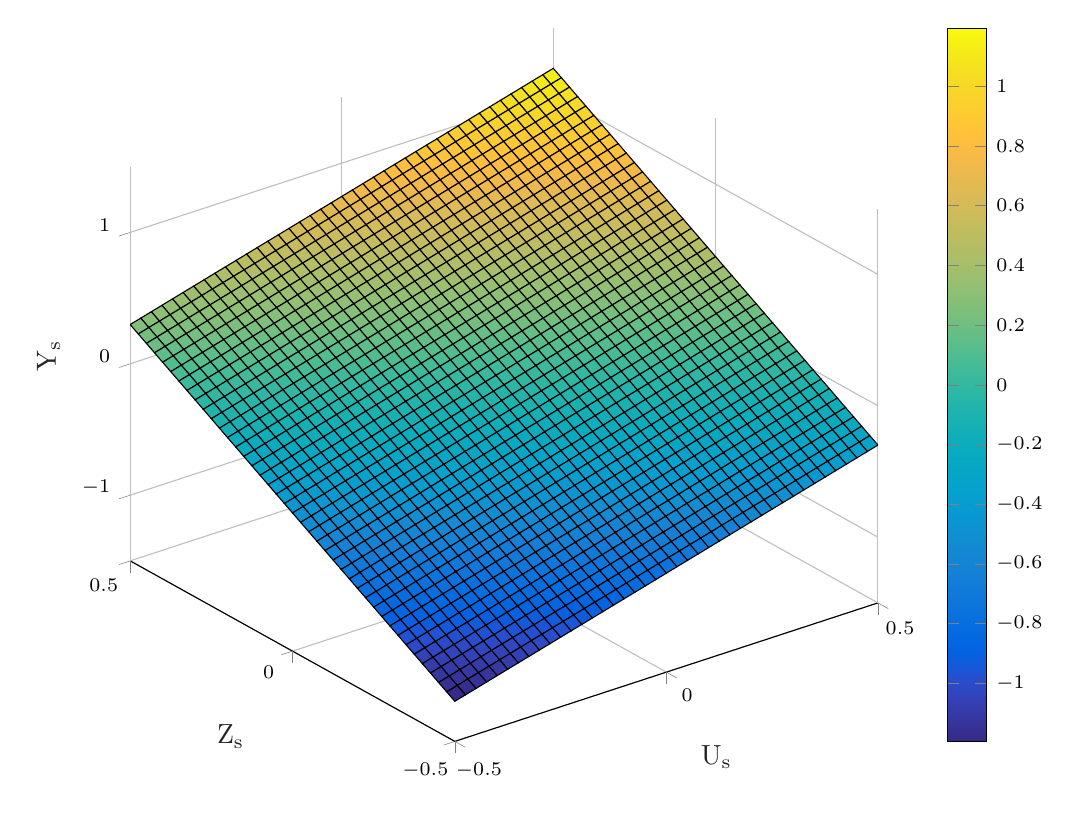
\begin{tikzpicture}

\begin{axis}[%
width=3.739in,
height=3.566in,
at={(0.66in,0.481in)},
scale only axis,
point meta min=-1.19475463603141,
point meta max=1.19475463603141,
xmin=-0.5,
xmax=0.5,
xtick={-0.5,0,0.5},
tick align=outside,
xlabel style={font=\color{white!15!black}},
xlabel={$\text{U}_\text{s}$},
ymin=-0.5,
ymax=0.5,
ytick={-0.5,0,0.5},
ylabel style={font=\color{white!15!black}},
ylabel={$\text{Z}_\text{s}$},
zmin=-1.5,
zmax=1.5,
zlabel style={font=\color{white!15!black}},
zlabel={$\text{Y}_\text{s}$},
view={-37.5}{30},
axis background/.style={fill=white},
axis x line*=bottom,
axis y line*=left,
axis z line*=left,
xmajorgrids,
ymajorgrids,
zmajorgrids,
colormap={mymap}{[1pt] rgb(0pt)=(0.2081,0.1663,0.5292); rgb(1pt)=(0.211624,0.189781,0.577676); rgb(2pt)=(0.212252,0.213771,0.626971); rgb(3pt)=(0.2081,0.2386,0.677086); rgb(4pt)=(0.195905,0.264457,0.7279); rgb(5pt)=(0.170729,0.291938,0.779248); rgb(6pt)=(0.125271,0.324243,0.830271); rgb(7pt)=(0.0591333,0.359833,0.868333); rgb(8pt)=(0.0116952,0.38751,0.881957); rgb(9pt)=(0.00595714,0.408614,0.882843); rgb(10pt)=(0.0165143,0.4266,0.878633); rgb(11pt)=(0.0328524,0.443043,0.871957); rgb(12pt)=(0.0498143,0.458571,0.864057); rgb(13pt)=(0.0629333,0.47369,0.855438); rgb(14pt)=(0.0722667,0.488667,0.8467); rgb(15pt)=(0.0779429,0.503986,0.838371); rgb(16pt)=(0.0793476,0.520024,0.831181); rgb(17pt)=(0.0749429,0.537543,0.826271); rgb(18pt)=(0.0640571,0.556986,0.823957); rgb(19pt)=(0.0487714,0.577224,0.822829); rgb(20pt)=(0.0343429,0.596581,0.819852); rgb(21pt)=(0.0265,0.6137,0.8135); rgb(22pt)=(0.0238905,0.628662,0.803762); rgb(23pt)=(0.0230905,0.641786,0.791267); rgb(24pt)=(0.0227714,0.653486,0.776757); rgb(25pt)=(0.0266619,0.664195,0.760719); rgb(26pt)=(0.0383714,0.674271,0.743552); rgb(27pt)=(0.0589714,0.683757,0.725386); rgb(28pt)=(0.0843,0.692833,0.706167); rgb(29pt)=(0.113295,0.7015,0.685857); rgb(30pt)=(0.145271,0.709757,0.664629); rgb(31pt)=(0.180133,0.717657,0.642433); rgb(32pt)=(0.217829,0.725043,0.619262); rgb(33pt)=(0.258643,0.731714,0.595429); rgb(34pt)=(0.302171,0.737605,0.571186); rgb(35pt)=(0.348167,0.742433,0.547267); rgb(36pt)=(0.395257,0.7459,0.524443); rgb(37pt)=(0.44201,0.748081,0.503314); rgb(38pt)=(0.487124,0.749062,0.483976); rgb(39pt)=(0.530029,0.749114,0.466114); rgb(40pt)=(0.570857,0.748519,0.44939); rgb(41pt)=(0.609852,0.747314,0.433686); rgb(42pt)=(0.6473,0.7456,0.4188); rgb(43pt)=(0.683419,0.743476,0.404433); rgb(44pt)=(0.71841,0.741133,0.390476); rgb(45pt)=(0.752486,0.7384,0.376814); rgb(46pt)=(0.785843,0.735567,0.363271); rgb(47pt)=(0.818505,0.732733,0.34979); rgb(48pt)=(0.850657,0.7299,0.336029); rgb(49pt)=(0.882433,0.727433,0.3217); rgb(50pt)=(0.913933,0.725786,0.306276); rgb(51pt)=(0.944957,0.726114,0.288643); rgb(52pt)=(0.973895,0.731395,0.266648); rgb(53pt)=(0.993771,0.745457,0.240348); rgb(54pt)=(0.999043,0.765314,0.216414); rgb(55pt)=(0.995533,0.786057,0.196652); rgb(56pt)=(0.988,0.8066,0.179367); rgb(57pt)=(0.978857,0.827143,0.163314); rgb(58pt)=(0.9697,0.848138,0.147452); rgb(59pt)=(0.962586,0.870514,0.1309); rgb(60pt)=(0.958871,0.8949,0.113243); rgb(61pt)=(0.959824,0.921833,0.0948381); rgb(62pt)=(0.9661,0.951443,0.0755333); rgb(63pt)=(0.9763,0.9831,0.0538)},
colorbar
]

\addplot3[%
surf,
shader=flat corner, draw=black, z buffer=sort, colormap={mymap}{[1pt] rgb(0pt)=(0.2081,0.1663,0.5292); rgb(1pt)=(0.211624,0.189781,0.577676); rgb(2pt)=(0.212252,0.213771,0.626971); rgb(3pt)=(0.2081,0.2386,0.677086); rgb(4pt)=(0.195905,0.264457,0.7279); rgb(5pt)=(0.170729,0.291938,0.779248); rgb(6pt)=(0.125271,0.324243,0.830271); rgb(7pt)=(0.0591333,0.359833,0.868333); rgb(8pt)=(0.0116952,0.38751,0.881957); rgb(9pt)=(0.00595714,0.408614,0.882843); rgb(10pt)=(0.0165143,0.4266,0.878633); rgb(11pt)=(0.0328524,0.443043,0.871957); rgb(12pt)=(0.0498143,0.458571,0.864057); rgb(13pt)=(0.0629333,0.47369,0.855438); rgb(14pt)=(0.0722667,0.488667,0.8467); rgb(15pt)=(0.0779429,0.503986,0.838371); rgb(16pt)=(0.0793476,0.520024,0.831181); rgb(17pt)=(0.0749429,0.537543,0.826271); rgb(18pt)=(0.0640571,0.556986,0.823957); rgb(19pt)=(0.0487714,0.577224,0.822829); rgb(20pt)=(0.0343429,0.596581,0.819852); rgb(21pt)=(0.0265,0.6137,0.8135); rgb(22pt)=(0.0238905,0.628662,0.803762); rgb(23pt)=(0.0230905,0.641786,0.791267); rgb(24pt)=(0.0227714,0.653486,0.776757); rgb(25pt)=(0.0266619,0.664195,0.760719); rgb(26pt)=(0.0383714,0.674271,0.743552); rgb(27pt)=(0.0589714,0.683757,0.725386); rgb(28pt)=(0.0843,0.692833,0.706167); rgb(29pt)=(0.113295,0.7015,0.685857); rgb(30pt)=(0.145271,0.709757,0.664629); rgb(31pt)=(0.180133,0.717657,0.642433); rgb(32pt)=(0.217829,0.725043,0.619262); rgb(33pt)=(0.258643,0.731714,0.595429); rgb(34pt)=(0.302171,0.737605,0.571186); rgb(35pt)=(0.348167,0.742433,0.547267); rgb(36pt)=(0.395257,0.7459,0.524443); rgb(37pt)=(0.44201,0.748081,0.503314); rgb(38pt)=(0.487124,0.749062,0.483976); rgb(39pt)=(0.530029,0.749114,0.466114); rgb(40pt)=(0.570857,0.748519,0.44939); rgb(41pt)=(0.609852,0.747314,0.433686); rgb(42pt)=(0.6473,0.7456,0.4188); rgb(43pt)=(0.683419,0.743476,0.404433); rgb(44pt)=(0.71841,0.741133,0.390476); rgb(45pt)=(0.752486,0.7384,0.376814); rgb(46pt)=(0.785843,0.735567,0.363271); rgb(47pt)=(0.818505,0.732733,0.34979); rgb(48pt)=(0.850657,0.7299,0.336029); rgb(49pt)=(0.882433,0.727433,0.3217); rgb(50pt)=(0.913933,0.725786,0.306276); rgb(51pt)=(0.944957,0.726114,0.288643); rgb(52pt)=(0.973895,0.731395,0.266648); rgb(53pt)=(0.993771,0.745457,0.240348); rgb(54pt)=(0.999043,0.765314,0.216414); rgb(55pt)=(0.995533,0.786057,0.196652); rgb(56pt)=(0.988,0.8066,0.179367); rgb(57pt)=(0.978857,0.827143,0.163314); rgb(58pt)=(0.9697,0.848138,0.147452); rgb(59pt)=(0.962586,0.870514,0.1309); rgb(60pt)=(0.958871,0.8949,0.113243); rgb(61pt)=(0.959824,0.921833,0.0948381); rgb(62pt)=(0.9661,0.951443,0.0755333); rgb(63pt)=(0.9763,0.9831,0.0538)}, mesh/rows=41]
table[row sep=crcr, point meta=\thisrow{c}] {%
%
x	y	z	c\\
-0.5	-0.5	-1.19475463603141	-1.19475463603141\\
-0.5	-0.475	-1.15741361254645	-1.15741361254645\\
-0.5	-0.45	-1.12007258906149	-1.12007258906149\\
-0.5	-0.425	-1.08273156557656	-1.08273156557656\\
-0.5	-0.4	-1.0453905420916	-1.0453905420916\\
-0.5	-0.375	-1.00804951860663	-1.00804951860663\\
-0.5	-0.35	-0.970708495121707	-0.970708495121707\\
-0.5	-0.325	-0.933367471636742	-0.933367471636742\\
-0.5	-0.3	-0.896026448151778	-0.896026448151778\\
-0.5	-0.275	-0.858685424666838	-0.858685424666838\\
-0.5	-0.25	-0.821344401181891	-0.821344401181891\\
-0.5	-0.225	-0.784003377696925	-0.784003377696925\\
-0.5	-0.2	-0.746662354211964	-0.746662354211964\\
-0.5	-0.175	-0.709321330727038	-0.709321330727038\\
-0.5	-0.15	-0.671980307242073	-0.671980307242073\\
-0.5	-0.125	-0.634639283757112	-0.634639283757112\\
-0.5	-0.1	-0.597298260272184	-0.597298260272184\\
-0.5	-0.075	-0.559957236787219	-0.559957236787219\\
-0.5	-0.05	-0.522616213302278	-0.522616213302278\\
-0.5	-0.025	-0.485275189817313	-0.485275189817313\\
-0.5	0	-0.447934166332367	-0.447934166332367\\
-0.5	0.025	-0.410593142847422	-0.410593142847422\\
-0.5	0.05	-0.37325211936246	-0.37325211936246\\
-0.5	0.0750000000000001	-0.335911095877514	-0.335911095877514\\
-0.5	0.1	-0.298570072392568	-0.298570072392568\\
-0.5	0.125	-0.26122904890761	-0.26122904890761\\
-0.5	0.15	-0.223888025422661	-0.223888025422661\\
-0.5	0.175	-0.186547001937707	-0.186547001937707\\
-0.5	0.2	-0.149205978452753	-0.149205978452753\\
-0.5	0.225	-0.111864954967803	-0.111864954967803\\
-0.5	0.25	-0.0745239314828537	-0.0745239314828537\\
-0.5	0.275	-0.0371829079979023	-0.0371829079979023\\
-0.5	0.3	0.000158115487049622	0.000158115487049622\\
-0.5	0.325	0.0374991389720015	0.0374991389720015\\
-0.5	0.35	0.0748401624569533	0.0748401624569533\\
-0.5	0.375	0.112181185941905	0.112181185941905\\
-0.5	0.4	0.149522209426852	0.149522209426852\\
-0.5	0.425	0.186863232911806	0.186863232911806\\
-0.5	0.45	0.224204256396761	0.224204256396761\\
-0.5	0.475	0.261545279881714	0.261545279881714\\
-0.5	0.5	0.298886303366662	0.298886303366662\\
-0.475	-0.5	-1.17235792771474	-1.17235792771474\\
-0.475	-0.475	-1.13501690422986	-1.13501690422986\\
-0.475	-0.45	-1.0976758807449	-1.0976758807449\\
-0.475	-0.425	-1.06033485725993	-1.06033485725993\\
-0.475	-0.4	-1.02299383377497	-1.02299383377497\\
-0.475	-0.375	-0.985652810290044	-0.985652810290044\\
-0.475	-0.35	-0.948311786805072	-0.948311786805072\\
-0.475	-0.325	-0.910970763320112	-0.910970763320112\\
-0.475	-0.3	-0.87362973983517	-0.87362973983517\\
-0.475	-0.275	-0.836288716350225	-0.836288716350225\\
-0.475	-0.25	-0.798947692865258	-0.798947692865258\\
-0.475	-0.225	-0.761606669380297	-0.761606669380297\\
-0.475	-0.2	-0.724265645895368	-0.724265645895368\\
-0.475	-0.175	-0.686924622410408	-0.686924622410408\\
-0.475	-0.15	-0.649583598925443	-0.649583598925443\\
-0.475	-0.125	-0.612242575440521	-0.612242575440521\\
-0.475	-0.1	-0.574901551955556	-0.574901551955556\\
-0.475	-0.075	-0.53756052847061	-0.53756052847061\\
-0.475	-0.05	-0.500219504985644	-0.500219504985644\\
-0.475	-0.025	-0.4628784815007	-0.4628784815007\\
-0.475	0	-0.425537458015757	-0.425537458015757\\
-0.475	0.025	-0.388196434530792	-0.388196434530792\\
-0.475	0.05	-0.350855411045849	-0.350855411045849\\
-0.475	0.0750000000000001	-0.313514387560903	-0.313514387560903\\
-0.475	0.1	-0.27617336407594	-0.27617336407594\\
-0.475	0.125	-0.238832340590995	-0.238832340590995\\
-0.475	0.15	-0.201491317106041	-0.201491317106041\\
-0.475	0.175	-0.164150293621087	-0.164150293621087\\
-0.475	0.2	-0.126809270136137	-0.126809270136137\\
-0.475	0.225	-0.0894682466511879	-0.0894682466511879\\
-0.475	0.25	-0.0521272231662361	-0.0521272231662361\\
-0.475	0.275	-0.0147861996812843	-0.0147861996812843\\
-0.475	0.3	0.0225548238036676	0.0225548238036676\\
-0.475	0.325	0.0598958472886196	0.0598958472886196\\
-0.475	0.35	0.0972368707735709	0.0972368707735709\\
-0.475	0.375	0.134577894258523	0.134577894258523\\
-0.475	0.4	0.171918917743473	0.171918917743473\\
-0.475	0.425	0.209259941228427	0.209259941228427\\
-0.475	0.45	0.246600964713376	0.246600964713376\\
-0.475	0.475	0.283941988198326	0.283941988198326\\
-0.475	0.5	0.32128301168328	0.32128301168328\\
-0.45	-0.5	-1.14996121939816	-1.14996121939816\\
-0.45	-0.475	-1.11262019591319	-1.11262019591319\\
-0.45	-0.45	-1.07527917242827	-1.07527917242827\\
-0.45	-0.425	-1.0379381489433	-1.0379381489433\\
-0.45	-0.4	-1.00059712545835	-1.00059712545835\\
-0.45	-0.375	-0.963256101973411	-0.963256101973411\\
-0.45	-0.35	-0.925915078488445	-0.925915078488445\\
-0.45	-0.325	-0.888574055003485	-0.888574055003485\\
-0.45	-0.3	-0.851233031518557	-0.851233031518557\\
-0.45	-0.275	-0.813892008033595	-0.813892008033595\\
-0.45	-0.25	-0.776550984548629	-0.776550984548629\\
-0.45	-0.225	-0.739209961063704	-0.739209961063704\\
-0.45	-0.2	-0.701868937578742	-0.701868937578742\\
-0.45	-0.175	-0.664527914093779	-0.664527914093779\\
-0.45	-0.15	-0.627186890608855	-0.627186890608855\\
-0.45	-0.125	-0.58984586712389	-0.58984586712389\\
-0.45	-0.1	-0.552504843638926	-0.552504843638926\\
-0.45	-0.075	-0.515163820153982	-0.515163820153982\\
-0.45	-0.05	-0.477822796669036	-0.477822796669036\\
-0.45	-0.025	-0.44048177318409	-0.44048177318409\\
-0.45	0	-0.403140749699126	-0.403140749699126\\
-0.45	0.025	-0.365799726214181	-0.365799726214181\\
-0.45	0.05	-0.328458702729238	-0.328458702729238\\
-0.45	0.0750000000000001	-0.291117679244273	-0.291117679244273\\
-0.45	0.1	-0.25377665575933	-0.25377665575933\\
-0.45	0.125	-0.216435632274375	-0.216435632274375\\
-0.45	0.15	-0.17909460878942	-0.17909460878942\\
-0.45	0.175	-0.141753585304472	-0.141753585304472\\
-0.45	0.2	-0.10441256181952	-0.10441256181952\\
-0.45	0.225	-0.0670715383345678	-0.0670715383345678\\
-0.45	0.25	-0.0297305148496169	-0.0297305148496169\\
-0.45	0.275	0.00761050863533476	0.00761050863533476\\
-0.45	0.3	0.0449515321202862	0.0449515321202862\\
-0.45	0.325	0.0822925556052398	0.0822925556052398\\
-0.45	0.35	0.119633579090189	0.119633579090189\\
-0.45	0.375	0.156974602575139	0.156974602575139\\
-0.45	0.4	0.194315626060092	0.194315626060092\\
-0.45	0.425	0.231656649545047	0.231656649545047\\
-0.45	0.45	0.268997673029992	0.268997673029992\\
-0.45	0.475	0.306338696514954	0.306338696514954\\
-0.45	0.5	0.343679719999899	0.343679719999899\\
-0.425	-0.5	-1.12756451108156	-1.12756451108156\\
-0.425	-0.475	-1.09022348759658	-1.09022348759658\\
-0.425	-0.45	-1.05288246411163	-1.05288246411163\\
-0.425	-0.425	-1.01554144062669	-1.01554144062669\\
-0.425	-0.4	-0.978200417141748	-0.978200417141748\\
-0.425	-0.375	-0.940859393656779	-0.940859393656779\\
-0.425	-0.35	-0.903518370171817	-0.903518370171817\\
-0.425	-0.325	-0.866177346686892	-0.866177346686892\\
-0.425	-0.3	-0.82883632320193	-0.82883632320193\\
-0.425	-0.275	-0.791495299716968	-0.791495299716968\\
-0.425	-0.25	-0.754154276232038	-0.754154276232038\\
-0.425	-0.225	-0.716813252747075	-0.716813252747075\\
-0.425	-0.2	-0.679472229262112	-0.679472229262112\\
-0.425	-0.175	-0.642131205777187	-0.642131205777187\\
-0.425	-0.15	-0.604790182292222	-0.604790182292222\\
-0.425	-0.125	-0.567449158807258	-0.567449158807258\\
-0.425	-0.1	-0.530108135322313	-0.530108135322313\\
-0.425	-0.075	-0.49276711183737	-0.49276711183737\\
-0.425	-0.05	-0.455426088352424	-0.455426088352424\\
-0.425	-0.025	-0.41808506486746	-0.41808506486746\\
-0.425	0	-0.380744041382516	-0.380744041382516\\
-0.425	0.025	-0.343403017897563	-0.343403017897563\\
-0.425	0.05	-0.306061994412608	-0.306061994412608\\
-0.425	0.0750000000000001	-0.268720970927662	-0.268720970927662\\
-0.425	0.1	-0.231379947442709	-0.231379947442709\\
-0.425	0.125	-0.194038923957754	-0.194038923957754\\
-0.425	0.15	-0.1566979004728	-0.1566979004728\\
-0.425	0.175	-0.119356876987853	-0.119356876987853\\
-0.425	0.2	-0.0820158535029017	-0.0820158535029017\\
-0.425	0.225	-0.0446748300179497	-0.0446748300179497\\
-0.425	0.25	-0.00733380653299909	-0.00733380653299909\\
-0.425	0.275	0.0300072169519527	0.0300072169519527\\
-0.425	0.3	0.0673482404369048	0.0673482404369048\\
-0.425	0.325	0.104689263921855	0.104689263921855\\
-0.425	0.35	0.142030287406805	0.142030287406805\\
-0.425	0.375	0.179371310891759	0.179371310891759\\
-0.425	0.4	0.216712334376713	0.216712334376713\\
-0.425	0.425	0.254053357861663	0.254053357861663\\
-0.425	0.45	0.291394381346622	0.291394381346622\\
-0.425	0.475	0.328735404831566	0.328735404831566\\
-0.425	0.5	0.366076428316511	0.366076428316511\\
-0.4	-0.5	-1.10516780276489	-1.10516780276489\\
-0.4	-0.475	-1.06782677927997	-1.06782677927997\\
-0.4	-0.45	-1.03048575579503	-1.03048575579503\\
-0.4	-0.425	-0.993144732310077	-0.993144732310077\\
-0.4	-0.4	-0.955803708825115	-0.955803708825115\\
-0.4	-0.375	-0.91846268534015	-0.91846268534015\\
-0.4	-0.35	-0.881121661855223	-0.881121661855223\\
-0.4	-0.325	-0.843780638370264	-0.843780638370264\\
-0.4	-0.3	-0.806439614885298	-0.806439614885298\\
-0.4	-0.275	-0.76909859140037	-0.76909859140037\\
-0.4	-0.25	-0.731757567915406	-0.731757567915406\\
-0.4	-0.225	-0.694416544430446	-0.694416544430446\\
-0.4	-0.2	-0.65707552094552	-0.65707552094552\\
-0.4	-0.175	-0.619734497460555	-0.619734497460555\\
-0.4	-0.15	-0.58239347397559	-0.58239347397559\\
-0.4	-0.125	-0.545052450490658	-0.545052450490658\\
-0.4	-0.1	-0.507711427005703	-0.507711427005703\\
-0.4	-0.075	-0.470370403520757	-0.470370403520757\\
-0.4	-0.05	-0.433029380035796	-0.433029380035796\\
-0.4	-0.025	-0.395688356550849	-0.395688356550849\\
-0.4	0	-0.358347333065896	-0.358347333065896\\
-0.4	0.025	-0.321006309580941	-0.321006309580941\\
-0.4	0.05	-0.283665286095997	-0.283665286095997\\
-0.4	0.0750000000000001	-0.246324262611043	-0.246324262611043\\
-0.4	0.1	-0.208983239126088	-0.208983239126088\\
-0.4	0.125	-0.171642215641134	-0.171642215641134\\
-0.4	0.15	-0.134301192156187	-0.134301192156187\\
-0.4	0.175	-0.0969601686712352	-0.0969601686712352\\
-0.4	0.2	-0.0596191451862834	-0.0596191451862834\\
-0.4	0.225	-0.0222781217013318	-0.0222781217013318\\
-0.4	0.25	0.0150629017836199	0.0150629017836199\\
-0.4	0.275	0.0524039252685708	0.0524039252685708\\
-0.4	0.3	0.0897449487535214	0.0897449487535214\\
-0.4	0.325	0.127085972238473	0.127085972238473\\
-0.4	0.35	0.164426995723424	0.164426995723424\\
-0.4	0.375	0.201768019208379	0.201768019208379\\
-0.4	0.4	0.239109042693328	0.239109042693328\\
-0.4	0.425	0.276450066178287	0.276450066178287\\
-0.4	0.45	0.313791089663232	0.313791089663232\\
-0.4	0.475	0.351132113148177	0.351132113148177\\
-0.4	0.5	0.388473136633142	0.388473136633142\\
-0.375	-0.5	-1.0827710944483	-1.0827710944483\\
-0.375	-0.475	-1.04543007096334	-1.04543007096334\\
-0.375	-0.45	-1.00808904747841	-1.00808904747841\\
-0.375	-0.425	-0.970748023993449	-0.970748023993449\\
-0.375	-0.4	-0.933407000508485	-0.933407000508485\\
-0.375	-0.375	-0.89606597702356	-0.89606597702356\\
-0.375	-0.35	-0.858724953538596	-0.858724953538596\\
-0.375	-0.325	-0.821383930053633	-0.821383930053633\\
-0.375	-0.3	-0.784042906568705	-0.784042906568705\\
-0.375	-0.275	-0.746701883083745	-0.746701883083745\\
-0.375	-0.25	-0.709360859598781	-0.709360859598781\\
-0.375	-0.225	-0.672019836113851	-0.672019836113851\\
-0.375	-0.2	-0.634678812628885	-0.634678812628885\\
-0.375	-0.175	-0.597337789143927	-0.597337789143927\\
-0.375	-0.15	-0.559996765658999	-0.559996765658999\\
-0.375	-0.125	-0.522655742174036	-0.522655742174036\\
-0.375	-0.1	-0.485314718689082	-0.485314718689082\\
-0.375	-0.075	-0.447973695204128	-0.447973695204128\\
-0.375	-0.05	-0.410632671719184	-0.410632671719184\\
-0.375	-0.025	-0.37329164823422	-0.37329164823422\\
-0.375	0	-0.335950624749276	-0.335950624749276\\
-0.375	0.025	-0.298609601264331	-0.298609601264331\\
-0.375	0.05	-0.261268577779376	-0.261268577779376\\
-0.375	0.0750000000000001	-0.223927554294422	-0.223927554294422\\
-0.375	0.1	-0.186586530809468	-0.186586530809468\\
-0.375	0.125	-0.149245507324519	-0.149245507324519\\
-0.375	0.15	-0.111904483839566	-0.111904483839566\\
-0.375	0.175	-0.0745634603546153	-0.0745634603546153\\
-0.375	0.2	-0.0372224368696646	-0.0372224368696646\\
-0.375	0.225	0.000118586615287216	0.000118586615287216\\
-0.375	0.25	0.0374596101002377	0.0374596101002377\\
-0.375	0.275	0.07480063358519	0.07480063358519\\
-0.375	0.3	0.112141657070142	0.112141657070142\\
-0.375	0.325	0.149482680555091	0.149482680555091\\
-0.375	0.35	0.186823704040044	0.186823704040044\\
-0.375	0.375	0.224164727524999	0.224164727524999\\
-0.375	0.4	0.261505751009943	0.261505751009943\\
-0.375	0.425	0.298846774494898	0.298846774494898\\
-0.375	0.45	0.336187797979843	0.336187797979843\\
-0.375	0.475	0.373528821464807	0.373528821464807\\
-0.375	0.5	0.41086984494975	0.41086984494975\\
-0.35	-0.5	-1.06037438613167	-1.06037438613167\\
-0.35	-0.475	-1.02303336264675	-1.02303336264675\\
-0.35	-0.45	-0.985692339161782	-0.985692339161782\\
-0.35	-0.425	-0.948351315676821	-0.948351315676821\\
-0.35	-0.4	-0.911010292191893	-0.911010292191893\\
-0.35	-0.375	-0.873669268706928	-0.873669268706928\\
-0.35	-0.35	-0.836328245221966	-0.836328245221966\\
-0.35	-0.325	-0.79898722173704	-0.79898722173704\\
-0.35	-0.3	-0.761646198252075	-0.761646198252075\\
-0.35	-0.275	-0.724305174767114	-0.724305174767114\\
-0.35	-0.25	-0.686964151282185	-0.686964151282185\\
-0.35	-0.225	-0.649623127797224	-0.649623127797224\\
-0.35	-0.2	-0.61228210431226	-0.61228210431226\\
-0.35	-0.175	-0.574941080827337	-0.574941080827337\\
-0.35	-0.15	-0.53760005734237	-0.53760005734237\\
-0.35	-0.125	-0.500259033857406	-0.500259033857406\\
-0.35	-0.1	-0.462918010372463	-0.462918010372463\\
-0.35	-0.075	-0.425576986887519	-0.425576986887519\\
-0.35	-0.05	-0.388235963402552	-0.388235963402552\\
-0.35	-0.025	-0.350894939917608	-0.350894939917608\\
-0.35	0	-0.313553916432665	-0.313553916432665\\
-0.35	0.025	-0.276212892947701	-0.276212892947701\\
-0.35	0.05	-0.238871869462756	-0.238871869462756\\
-0.35	0.0750000000000001	-0.201530845977802	-0.201530845977802\\
-0.35	0.1	-0.164189822492848	-0.164189822492848\\
-0.35	0.125	-0.126848799007899	-0.126848799007899\\
-0.35	0.15	-0.0895077755229489	-0.0895077755229489\\
-0.35	0.175	-0.0521667520379975	-0.0521667520379975\\
-0.35	0.2	-0.0148257285530455	-0.0148257285530455\\
-0.35	0.225	0.0225152949319062	0.0225152949319062\\
-0.35	0.25	0.0598563184168573	0.0598563184168573\\
-0.35	0.275	0.0971973419018076	0.0971973419018076\\
-0.35	0.3	0.134538365386762	0.134538365386762\\
-0.35	0.325	0.171879388871711	0.171879388871711\\
-0.35	0.35	0.209220412356666	0.209220412356666\\
-0.35	0.375	0.246561435841619	0.246561435841619\\
-0.35	0.4	0.283902459326564	0.283902459326564\\
-0.35	0.425	0.321243482811517	0.321243482811517\\
-0.35	0.45	0.358584506296473	0.358584506296473\\
-0.35	0.475	0.395925529781418	0.395925529781418\\
-0.35	0.5	0.43326655326638	0.43326655326638\\
-0.325	-0.5	-1.03797767781508	-1.03797767781508\\
-0.325	-0.475	-1.00063665433012	-1.00063665433012\\
-0.325	-0.45	-0.963295630845151	-0.963295630845151\\
-0.325	-0.425	-0.92595460736023	-0.92595460736023\\
-0.325	-0.4	-0.888613583875265	-0.888613583875265\\
-0.325	-0.375	-0.851272560390302	-0.851272560390302\\
-0.325	-0.35	-0.813931536905375	-0.813931536905375\\
-0.325	-0.325	-0.776590513420411	-0.776590513420411\\
-0.325	-0.3	-0.739249489935445	-0.739249489935445\\
-0.325	-0.275	-0.70190846645052	-0.70190846645052\\
-0.325	-0.25	-0.664567442965561	-0.664567442965561\\
-0.325	-0.225	-0.627226419480596	-0.627226419480596\\
-0.325	-0.2	-0.589885395995671	-0.589885395995671\\
-0.325	-0.175	-0.552544372510705	-0.552544372510705\\
-0.325	-0.15	-0.51520334902574	-0.51520334902574\\
-0.325	-0.125	-0.477862325540797	-0.477862325540797\\
-0.325	-0.1	-0.440521302055853	-0.440521302055853\\
-0.325	-0.075	-0.403180278570888	-0.403180278570888\\
-0.325	-0.05	-0.365839255085942	-0.365839255085942\\
-0.325	-0.025	-0.328498231600999	-0.328498231600999\\
-0.325	0	-0.291157208116035	-0.291157208116035\\
-0.325	0.025	-0.253816184631091	-0.253816184631091\\
-0.325	0.05	-0.216475161146136	-0.216475161146136\\
-0.325	0.0750000000000001	-0.179134137661183	-0.179134137661183\\
-0.325	0.1	-0.141793114176237	-0.141793114176237\\
-0.325	0.125	-0.104452090691283	-0.104452090691283\\
-0.325	0.15	-0.06711106720633	-0.06711106720633\\
-0.325	0.175	-0.0297700437213794	-0.0297700437213794\\
-0.325	0.2	0.00757097976357238	0.00757097976357238\\
-0.325	0.225	0.0449120032485242	0.0449120032485242\\
-0.325	0.25	0.0822530267334738	0.0822530267334738\\
-0.325	0.275	0.119594050218428	0.119594050218428\\
-0.325	0.3	0.156935073703377	0.156935073703377\\
-0.325	0.325	0.194276097188332	0.194276097188332\\
-0.325	0.35	0.231617120673285	0.231617120673285\\
-0.325	0.375	0.268958144158229	0.268958144158229\\
-0.325	0.4	0.306299167643183	0.306299167643183\\
-0.325	0.425	0.343640191128138	0.343640191128138\\
-0.325	0.45	0.380981214613083	0.380981214613083\\
-0.325	0.475	0.418322238098047	0.418322238098047\\
-0.325	0.5	0.455663261582992	0.455663261582992\\
-0.3	-0.5	-1.01558096949846	-1.01558096949846\\
-0.3	-0.475	-0.978239946013487	-0.978239946013487\\
-0.3	-0.45	-0.940898922528563	-0.940898922528563\\
-0.3	-0.425	-0.9035578990436	-0.9035578990436\\
-0.3	-0.4	-0.866216875558636	-0.866216875558636\\
-0.3	-0.375	-0.82887585207371	-0.82887585207371\\
-0.3	-0.35	-0.791534828588743	-0.791534828588743\\
-0.3	-0.325	-0.754193805103781	-0.754193805103781\\
-0.3	-0.3	-0.716852781618853	-0.716852781618853\\
-0.3	-0.275	-0.679511758133893	-0.679511758133893\\
-0.3	-0.25	-0.642170734648927	-0.642170734648927\\
-0.3	-0.225	-0.604829711163999	-0.604829711163999\\
-0.3	-0.2	-0.567488687679038	-0.567488687679038\\
-0.3	-0.175	-0.530147664194076	-0.530147664194076\\
-0.3	-0.15	-0.49280664070913	-0.49280664070913\\
-0.3	-0.125	-0.455465617224186	-0.455465617224186\\
-0.3	-0.1	-0.418124593739222	-0.418124593739222\\
-0.3	-0.075	-0.380783570254278	-0.380783570254278\\
-0.3	-0.05	-0.343442546769324	-0.343442546769324\\
-0.3	-0.025	-0.306101523284369	-0.306101523284369\\
-0.3	0	-0.268760499799425	-0.268760499799425\\
-0.3	0.025	-0.231419476314469	-0.231419476314469\\
-0.3	0.05	-0.194078452829516	-0.194078452829516\\
-0.3	0.0750000000000001	-0.156737429344561	-0.156737429344561\\
-0.3	0.1	-0.119396405859614	-0.119396405859614\\
-0.3	0.125	-0.0820553823746629	-0.0820553823746629\\
-0.3	0.15	-0.044714358889711	-0.044714358889711\\
-0.3	0.175	-0.00737333540476034	-0.00737333540476034\\
-0.3	0.2	0.0299676880801915	0.0299676880801915\\
-0.3	0.225	0.0673087115651432	0.0673087115651432\\
-0.3	0.25	0.104649735050094	0.104649735050094\\
-0.3	0.275	0.141990758535044	0.141990758535044\\
-0.3	0.3	0.179331782019998	0.179331782019998\\
-0.3	0.325	0.216672805504951	0.216672805504951\\
-0.3	0.35	0.254013828989897	0.254013828989897\\
-0.3	0.375	0.291354852474858	0.291354852474858\\
-0.3	0.4	0.328695875959804	0.328695875959804\\
-0.3	0.425	0.366036899444749	0.366036899444749\\
-0.3	0.45	0.403377922929714	0.403377922929714\\
-0.3	0.475	0.440718946414659	0.440718946414659\\
-0.3	0.5	0.478059969899603	0.478059969899603\\
-0.275	-0.5	-0.993184261181821	-0.993184261181821\\
-0.275	-0.475	-0.955843237696892	-0.955843237696892\\
-0.275	-0.45	-0.918502214211932	-0.918502214211932\\
-0.275	-0.425	-0.881161190726969	-0.881161190726969\\
-0.275	-0.4	-0.843820167242041	-0.843820167242041\\
-0.275	-0.375	-0.806479143757079	-0.806479143757079\\
-0.275	-0.35	-0.769138120272114	-0.769138120272114\\
-0.275	-0.325	-0.731797096787189	-0.731797096787189\\
-0.275	-0.3	-0.694456073302225	-0.694456073302225\\
-0.275	-0.275	-0.657115049817262	-0.657115049817262\\
-0.275	-0.25	-0.619774026332334	-0.619774026332334\\
-0.275	-0.225	-0.582433002847372	-0.582433002847372\\
-0.275	-0.2	-0.545091979362416	-0.545091979362416\\
-0.275	-0.175	-0.507750955877464	-0.507750955877464\\
-0.275	-0.15	-0.470409932392519	-0.470409932392519\\
-0.275	-0.125	-0.433068908907557	-0.433068908907557\\
-0.275	-0.1	-0.395727885422611	-0.395727885422611\\
-0.275	-0.075	-0.358386861937656	-0.358386861937656\\
-0.275	-0.05	-0.321045838452704	-0.321045838452704\\
-0.275	-0.025	-0.283704814967758	-0.283704814967758\\
-0.275	0	-0.246363791482804	-0.246363791482804\\
-0.275	0.025	-0.20902276799785	-0.20902276799785\\
-0.275	0.05	-0.171681744512895	-0.171681744512895\\
-0.275	0.0750000000000001	-0.134340721027946	-0.134340721027946\\
-0.275	0.1	-0.0969996975429965	-0.0969996975429965\\
-0.275	0.125	-0.059658674058045	-0.059658674058045\\
-0.275	0.15	-0.0223176505730938	-0.0223176505730938\\
-0.275	0.175	0.0150233729118575	0.0150233729118575\\
-0.275	0.2	0.0523643963968093	0.0523643963968093\\
-0.275	0.225	0.0897054198817597	0.0897054198817597\\
-0.275	0.25	0.127046443366714	0.127046443366714\\
-0.275	0.275	0.164387466851664	0.164387466851664\\
-0.275	0.3	0.201728490336618	0.201728490336618\\
-0.275	0.325	0.239069513821562	0.239069513821562\\
-0.275	0.35	0.276410537306526	0.276410537306526\\
-0.275	0.375	0.31375156079147	0.31375156079147\\
-0.275	0.4	0.351092584276416	0.351092584276416\\
-0.275	0.425	0.38843360776138	0.38843360776138\\
-0.275	0.45	0.425774631246323	0.425774631246323\\
-0.275	0.475	0.463115654731268	0.463115654731268\\
-0.275	0.5	0.500456678216231	0.500456678216231\\
-0.25	-0.5	-0.970787552865228	-0.970787552865228\\
-0.25	-0.475	-0.933446529380265	-0.933446529380265\\
-0.25	-0.45	-0.8961055058953	-0.8961055058953\\
-0.25	-0.425	-0.858764482410375	-0.858764482410375\\
-0.25	-0.4	-0.821423458925412	-0.821423458925412\\
-0.25	-0.375	-0.784082435440451	-0.784082435440451\\
-0.25	-0.35	-0.746741411955521	-0.746741411955521\\
-0.25	-0.325	-0.709400388470558	-0.709400388470558\\
-0.25	-0.3	-0.672059364985596	-0.672059364985596\\
-0.25	-0.275	-0.634718341500633	-0.634718341500633\\
-0.25	-0.25	-0.597377318015703	-0.597377318015703\\
-0.25	-0.225	-0.560036294530743	-0.560036294530743\\
-0.25	-0.2	-0.522695271045799	-0.522695271045799\\
-0.25	-0.175	-0.485354247560853	-0.485354247560853\\
-0.25	-0.15	-0.448013224075889	-0.448013224075889\\
-0.25	-0.125	-0.410672200590946	-0.410672200590946\\
-0.25	-0.1	-0.373331177105982	-0.373331177105982\\
-0.25	-0.075	-0.335990153621036	-0.335990153621036\\
-0.25	-0.05	-0.298649130136092	-0.298649130136092\\
-0.25	-0.025	-0.261308106651139	-0.261308106651139\\
-0.25	0	-0.223967083166183	-0.223967083166183\\
-0.25	0.025	-0.18662605968123	-0.18662605968123\\
-0.25	0.05	-0.149285036196284	-0.149285036196284\\
-0.25	0.0750000000000001	-0.11194401271133	-0.11194401271133\\
-0.25	0.1	-0.0746029892263765	-0.0746029892263765\\
-0.25	0.125	-0.0372619657414269	-0.0372619657414269\\
-0.25	0.15	7.90577435248108e-05	7.90577435248108e-05\\
-0.25	0.175	0.0374200812284766	0.0374200812284766\\
-0.25	0.2	0.0747611047134289	0.0747611047134289\\
-0.25	0.225	0.11210212819838	0.11210212819838\\
-0.25	0.25	0.149443151683331	0.149443151683331\\
-0.25	0.275	0.186784175168283	0.186784175168283\\
-0.25	0.3	0.224125198653238	0.224125198653238\\
-0.25	0.325	0.261466222138183	0.261466222138183\\
-0.25	0.35	0.298807245623137	0.298807245623137\\
-0.25	0.375	0.336148269108081	0.336148269108081\\
-0.25	0.4	0.373489292593044	0.373489292593044\\
-0.25	0.425	0.410830316077991	0.410830316077991\\
-0.25	0.45	0.448171339562935	0.448171339562935\\
-0.25	0.475	0.485512363047897	0.485512363047897\\
-0.25	0.5	0.522853386532843	0.522853386532843\\
-0.225	-0.5	-0.948390844548601	-0.948390844548601\\
-0.225	-0.475	-0.911049821063639	-0.911049821063639\\
-0.225	-0.45	-0.873708797578709	-0.873708797578709\\
-0.225	-0.425	-0.836367774093746	-0.836367774093746\\
-0.225	-0.4	-0.799026750608781	-0.799026750608781\\
-0.225	-0.375	-0.761685727123855	-0.761685727123855\\
-0.225	-0.35	-0.724344703638894	-0.724344703638894\\
-0.225	-0.325	-0.687003680153931	-0.687003680153931\\
-0.225	-0.3	-0.649662656668966	-0.649662656668966\\
-0.225	-0.275	-0.61232163318404	-0.61232163318404\\
-0.225	-0.25	-0.574980609699078	-0.574980609699078\\
-0.225	-0.225	-0.537639586214134	-0.537639586214134\\
-0.225	-0.2	-0.500298562729176	-0.500298562729176\\
-0.225	-0.175	-0.462957539244223	-0.462957539244223\\
-0.225	-0.15	-0.425616515759279	-0.425616515759279\\
-0.225	-0.125	-0.388275492274315	-0.388275492274315\\
-0.225	-0.1	-0.350934468789371	-0.350934468789371\\
-0.225	-0.075	-0.313593445304427	-0.313593445304427\\
-0.225	-0.05	-0.276252421819463	-0.276252421819463\\
-0.225	-0.025	-0.238911398334518	-0.238911398334518\\
-0.225	0	-0.201570374849563	-0.201570374849563\\
-0.225	0.025	-0.164229351364614	-0.164229351364614\\
-0.225	0.05	-0.126888327879665	-0.126888327879665\\
-0.225	0.0750000000000001	-0.0895473043947101	-0.0895473043947101\\
-0.225	0.1	-0.0522062809097598	-0.0522062809097598\\
-0.225	0.125	-0.0148652574248079	-0.0148652574248079\\
-0.225	0.15	0.0224757660601431	0.0224757660601431\\
-0.225	0.175	0.0598167895450947	0.0598167895450947\\
-0.225	0.2	0.0971578130300461	0.0971578130300461\\
-0.225	0.225	0.134498836514998	0.134498836514998\\
-0.225	0.25	0.17183985999995	0.17183985999995\\
-0.225	0.275	0.209180883484905	0.209180883484905\\
-0.225	0.3	0.246521906969849	0.246521906969849\\
-0.225	0.325	0.283862930454803	0.283862930454803\\
-0.225	0.35	0.321203953939748	0.321203953939748\\
-0.225	0.375	0.358544977424711	0.358544977424711\\
-0.225	0.4	0.395886000909657	0.395886000909657\\
-0.225	0.425	0.433227024394609	0.433227024394609\\
-0.225	0.45	0.470568047879566	0.470568047879566\\
-0.225	0.475	0.507909071364508	0.507909071364508\\
-0.225	0.5	0.545250094849467	0.545250094849467\\
-0.2	-0.5	-0.92599413623197	-0.92599413623197\\
-0.2	-0.475	-0.888653112747044	-0.888653112747044\\
-0.2	-0.45	-0.851312089262078	-0.851312089262078\\
-0.2	-0.425	-0.813971065777114	-0.813971065777114\\
-0.2	-0.4	-0.776630042292155	-0.776630042292155\\
-0.2	-0.375	-0.739289018807224	-0.739289018807224\\
-0.2	-0.35	-0.701947995322266	-0.701947995322266\\
-0.2	-0.325	-0.664606971837302	-0.664606971837302\\
-0.2	-0.3	-0.627265948352375	-0.627265948352375\\
-0.2	-0.275	-0.589924924867414	-0.589924924867414\\
-0.2	-0.25	-0.552583901382444	-0.552583901382444\\
-0.2	-0.225	-0.5152428778975	-0.5152428778975\\
-0.2	-0.2	-0.477901854412557	-0.477901854412557\\
-0.2	-0.175	-0.440560830927614	-0.440560830927614\\
-0.2	-0.15	-0.403219807442649	-0.403219807442649\\
-0.2	-0.125	-0.365878783957703	-0.365878783957703\\
-0.2	-0.1	-0.32853776047276	-0.32853776047276\\
-0.2	-0.075	-0.291196736987795	-0.291196736987795\\
-0.2	-0.05	-0.253855713502851	-0.253855713502851\\
-0.2	-0.025	-0.216514690017897	-0.216514690017897\\
-0.2	0	-0.179173666532943	-0.179173666532943\\
-0.2	0.025	-0.141832643047998	-0.141832643047998\\
-0.2	0.05	-0.104491619563044	-0.104491619563044\\
-0.2	0.0750000000000001	-0.0671505960780924	-0.0671505960780924\\
-0.2	0.1	-0.0298095725931413	-0.0298095725931413\\
-0.2	0.125	0.00753145089181056	0.00753145089181056\\
-0.2	0.15	0.044872474376762	0.044872474376762\\
-0.2	0.175	0.0822134978617122	0.0822134978617122\\
-0.2	0.2	0.119554521346666	0.119554521346666\\
-0.2	0.225	0.156895544831616	0.156895544831616\\
-0.2	0.25	0.19423656831657	0.19423656831657\\
-0.2	0.275	0.231577591801514	0.231577591801514\\
-0.2	0.3	0.26891861528647	0.26891861528647\\
-0.2	0.325	0.306259638771414	0.306259638771414\\
-0.2	0.35	0.343600662256378	0.343600662256378\\
-0.2	0.375	0.380941685741323	0.380941685741323\\
-0.2	0.4	0.418282709226286	0.418282709226286\\
-0.2	0.425	0.45562373271123	0.45562373271123\\
-0.2	0.45	0.492964756196175	0.492964756196175\\
-0.2	0.475	0.530305779681141	0.530305779681141\\
-0.2	0.5	0.567646803166082	0.567646803166082\\
-0.175	-0.5	-0.903597427915353	-0.903597427915353\\
-0.175	-0.475	-0.866256404430412	-0.866256404430412\\
-0.175	-0.45	-0.828915380945451	-0.828915380945451\\
-0.175	-0.425	-0.791574357460487	-0.791574357460487\\
-0.175	-0.4	-0.754233333975562	-0.754233333975562\\
-0.175	-0.375	-0.716892310490596	-0.716892310490596\\
-0.175	-0.35	-0.679551287005636	-0.679551287005636\\
-0.175	-0.325	-0.642210263520706	-0.642210263520706\\
-0.175	-0.3	-0.604869240035743	-0.604869240035743\\
-0.175	-0.275	-0.567528216550783	-0.567528216550783\\
-0.175	-0.25	-0.530187193065837	-0.530187193065837\\
-0.175	-0.225	-0.492846169580891	-0.492846169580891\\
-0.175	-0.2	-0.455505146095946	-0.455505146095946\\
-0.175	-0.175	-0.418164122610983	-0.418164122610983\\
-0.175	-0.15	-0.380823099126037	-0.380823099126037\\
-0.175	-0.125	-0.343482075641093	-0.343482075641093\\
-0.175	-0.1	-0.30614105215613	-0.30614105215613\\
-0.175	-0.075	-0.268800028671187	-0.268800028671187\\
-0.175	-0.05	-0.231459005186232	-0.231459005186232\\
-0.175	-0.025	-0.194117981701276	-0.194117981701276\\
-0.175	0	-0.156776958216333	-0.156776958216333\\
-0.175	0.025	-0.119435934731378	-0.119435934731378\\
-0.175	0.05	-0.0820949112464239	-0.0820949112464239\\
-0.175	0.0750000000000001	-0.0447538877614744	-0.0447538877614744\\
-0.175	0.1	-0.00741286427652275	-0.00741286427652275\\
-0.175	0.125	0.0299281592084287	0.0299281592084287\\
-0.175	0.15	0.0672691826933809	0.0672691826933809\\
-0.175	0.175	0.104610206178333	0.104610206178333\\
-0.175	0.2	0.141951229663283	0.141951229663283\\
-0.175	0.225	0.179292253148237	0.179292253148237\\
-0.175	0.25	0.21663327663319	0.21663327663319\\
-0.175	0.275	0.253974300118136	0.253974300118136\\
-0.175	0.3	0.29131532360309	0.29131532360309\\
-0.175	0.325	0.328656347088043	0.328656347088043\\
-0.175	0.35	0.365997370572989	0.365997370572989\\
-0.175	0.375	0.403338394057952	0.403338394057952\\
-0.175	0.4	0.440679417542897	0.440679417542897\\
-0.175	0.425	0.478020441027841	0.478020441027841\\
-0.175	0.45	0.515361464512805	0.515361464512805\\
-0.175	0.475	0.55270248799775	0.55270248799775\\
-0.175	0.5	0.590043511482713	0.590043511482713\\
-0.15	-0.5	-0.881200719598749	-0.881200719598749\\
-0.15	-0.475	-0.843859696113784	-0.843859696113784\\
-0.15	-0.45	-0.80651867262882	-0.80651867262882\\
-0.15	-0.425	-0.769177649143892	-0.769177649143892\\
-0.15	-0.4	-0.731836625658929	-0.731836625658929\\
-0.15	-0.375	-0.69449560217397	-0.69449560217397\\
-0.15	-0.35	-0.657154578689042	-0.657154578689042\\
-0.15	-0.325	-0.619813555204081	-0.619813555204081\\
-0.15	-0.3	-0.582472531719115	-0.582472531719115\\
-0.15	-0.275	-0.54513150823418	-0.54513150823418\\
-0.15	-0.25	-0.507790484749223	-0.507790484749223\\
-0.15	-0.225	-0.470449461264281	-0.470449461264281\\
-0.15	-0.2	-0.433108437779316	-0.433108437779316\\
-0.15	-0.175	-0.395767414294371	-0.395767414294371\\
-0.15	-0.15	-0.358426390809427	-0.358426390809427\\
-0.15	-0.125	-0.321085367324465	-0.321085367324465\\
-0.15	-0.1	-0.283744343839517	-0.283744343839517\\
-0.15	-0.075	-0.246403320354565	-0.246403320354565\\
-0.15	-0.05	-0.209062296869611	-0.209062296869611\\
-0.15	-0.025	-0.171721273384662	-0.171721273384662\\
-0.15	0	-0.134380249899712	-0.134380249899712\\
-0.15	0.025	-0.0970392264147581	-0.0970392264147581\\
-0.15	0.05	-0.0596982029298071	-0.0596982029298071\\
-0.15	0.0750000000000001	-0.0223571794448554	-0.0223571794448554\\
-0.15	0.1	0.0149838440400957	0.0149838440400957\\
-0.15	0.125	0.0523248675250469	0.0523248675250469\\
-0.15	0.15	0.089665891009999	0.089665891009999\\
-0.15	0.175	0.127006914494948	0.127006914494948\\
-0.15	0.2	0.164347937979901	0.164347937979901\\
-0.15	0.225	0.201688961464857	0.201688961464857\\
-0.15	0.25	0.239029984949802	0.239029984949802\\
-0.15	0.275	0.276371008434765	0.276371008434765\\
-0.15	0.3	0.31371203191971	0.31371203191971\\
-0.15	0.325	0.351053055404654	0.351053055404654\\
-0.15	0.35	0.388394078889618	0.388394078889618\\
-0.15	0.375	0.425735102374563	0.425735102374563\\
-0.15	0.4	0.463076125859507	0.463076125859507\\
-0.15	0.425	0.500417149344469	0.500417149344469\\
-0.15	0.45	0.537758172829414	0.537758172829414\\
-0.15	0.475	0.57509919631438	0.57509919631438\\
-0.15	0.5	0.612440219799306	0.612440219799306\\
-0.125	-0.5	-0.858804011282118	-0.858804011282118\\
-0.125	-0.475	-0.821462987797157	-0.821462987797157\\
-0.125	-0.45	-0.784121964312228	-0.784121964312228\\
-0.125	-0.425	-0.746780940827267	-0.746780940827267\\
-0.125	-0.4	-0.709439917342302	-0.709439917342302\\
-0.125	-0.375	-0.672098893857376	-0.672098893857376\\
-0.125	-0.35	-0.634757870372414	-0.634757870372414\\
-0.125	-0.325	-0.597416846887446	-0.597416846887446\\
-0.125	-0.3	-0.560075823402523	-0.560075823402523\\
-0.125	-0.275	-0.52273479991756	-0.52273479991756\\
-0.125	-0.25	-0.485393776432614	-0.485393776432614\\
-0.125	-0.225	-0.448052752947652	-0.448052752947652\\
-0.125	-0.2	-0.410711729462706	-0.410711729462706\\
-0.125	-0.175	-0.37337070597776	-0.37337070597776\\
-0.125	-0.15	-0.336029682492798	-0.336029682492798\\
-0.125	-0.125	-0.298688659007851	-0.298688659007851\\
-0.125	-0.1	-0.2613476355229	-0.2613476355229\\
-0.125	-0.075	-0.224006612037945	-0.224006612037945\\
-0.125	-0.05	-0.186665588552991	-0.186665588552991\\
-0.125	-0.025	-0.149324565068046	-0.149324565068046\\
-0.125	0	-0.111983541583092	-0.111983541583092\\
-0.125	0.025	-0.0746425180981419	-0.0746425180981419\\
-0.125	0.05	-0.0373014946131882	-0.0373014946131882\\
-0.125	0.0750000000000001	3.95288717624054e-05	3.95288717624054e-05\\
-0.125	0.1	0.0373805523567129	0.0373805523567129\\
-0.125	0.125	0.0747215758416654	0.0747215758416654\\
-0.125	0.15	0.112062599326619	0.112062599326619\\
-0.125	0.175	0.149403622811569	0.149403622811569\\
-0.125	0.2	0.186744646296522	0.186744646296522\\
-0.125	0.225	0.224085669781467	0.224085669781467\\
-0.125	0.25	0.261426693266421	0.261426693266421\\
-0.125	0.275	0.298767716751375	0.298767716751375\\
-0.125	0.3	0.33610874023632	0.33610874023632\\
-0.125	0.325	0.373449763721285	0.373449763721285\\
-0.125	0.35	0.410790787206229	0.410790787206229\\
-0.125	0.375	0.448131810691173	0.448131810691173\\
-0.125	0.4	0.485472834176137	0.485472834176137\\
-0.125	0.425	0.522813857661081	0.522813857661081\\
-0.125	0.45	0.560154881146046	0.560154881146046\\
-0.125	0.475	0.597495904630973	0.597495904630973\\
-0.125	0.5	0.634836928115934	0.634836928115934\\
-0.1	-0.5	-0.836407302965488	-0.836407302965488\\
-0.1	-0.475	-0.799066279480564	-0.799066279480564\\
-0.1	-0.45	-0.761725255995597	-0.761725255995597\\
-0.1	-0.425	-0.724384232510634	-0.724384232510634\\
-0.1	-0.4	-0.687043209025708	-0.687043209025708\\
-0.1	-0.375	-0.649702185540746	-0.649702185540746\\
-0.1	-0.35	-0.612361162055784	-0.612361162055784\\
-0.1	-0.325	-0.575020138570856	-0.575020138570856\\
-0.1	-0.3	-0.537679115085893	-0.537679115085893\\
-0.1	-0.275	-0.500338091600949	-0.500338091600949\\
-0.1	-0.25	-0.462997068115985	-0.462997068115985\\
-0.1	-0.225	-0.425656044631039	-0.425656044631039\\
-0.1	-0.2	-0.388315021146078	-0.388315021146078\\
-0.1	-0.175	-0.350973997661133	-0.350973997661133\\
-0.1	-0.15	-0.313632974176187	-0.313632974176187\\
-0.1	-0.125	-0.276291950691222	-0.276291950691222\\
-0.1	-0.1	-0.238950927206278	-0.238950927206278\\
-0.1	-0.075	-0.201609903721325	-0.201609903721325\\
-0.1	-0.05	-0.16426888023638	-0.16426888023638\\
-0.1	-0.025	-0.126927856751426	-0.126927856751426\\
-0.1	0	-0.0895868332664716	-0.0895868332664716\\
-0.1	0.025	-0.0522458097815222	-0.0522458097815222\\
-0.1	0.05	-0.0149047862965706	-0.0149047862965706\\
-0.1	0.0750000000000001	0.0224362371883814	0.0224362371883814\\
-0.1	0.1	0.0597772606733332	0.0597772606733332\\
-0.1	0.125	0.097118284158285	0.097118284158285\\
-0.1	0.15	0.134459307643235	0.134459307643235\\
-0.1	0.175	0.171800331128189	0.171800331128189\\
-0.1	0.2	0.209141354613143	0.209141354613143\\
-0.1	0.225	0.246482378098088	0.246482378098088\\
-0.1	0.25	0.283823401583041	0.283823401583041\\
-0.1	0.275	0.321164425067988	0.321164425067988\\
-0.1	0.3	0.35850544855295	0.35850544855295\\
-0.1	0.325	0.395846472037896	0.395846472037896\\
-0.1	0.35	0.43318749552284	0.43318749552284\\
-0.1	0.375	0.470528519007801	0.470528519007801\\
-0.1	0.4	0.507869542492746	0.507869542492746\\
-0.1	0.425	0.545210565977701	0.545210565977701\\
-0.1	0.45	0.582551589462637	0.582551589462637\\
-0.1	0.475	0.619892612947598	0.619892612947598\\
-0.1	0.5	0.657233636432565	0.657233636432565\\
-0.075	-0.5	-0.814010594648897	-0.814010594648897\\
-0.075	-0.475	-0.776669571163934	-0.776669571163934\\
-0.075	-0.45	-0.739328547678969	-0.739328547678969\\
-0.075	-0.425	-0.701987524194043	-0.701987524194043\\
-0.075	-0.4	-0.664646500709079	-0.664646500709079\\
-0.075	-0.375	-0.627305477224118	-0.627305477224118\\
-0.075	-0.35	-0.58996445373919	-0.58996445373919\\
-0.075	-0.325	-0.55262343025423	-0.55262343025423\\
-0.075	-0.3	-0.515282406769283	-0.515282406769283\\
-0.075	-0.275	-0.477941383284318	-0.477941383284318\\
-0.075	-0.25	-0.440600359799375	-0.440600359799375\\
-0.075	-0.225	-0.40325933631441	-0.40325933631441\\
-0.075	-0.2	-0.365918312829466	-0.365918312829466\\
-0.075	-0.175	-0.328577289344522	-0.328577289344522\\
-0.075	-0.15	-0.291236265859557	-0.291236265859557\\
-0.075	-0.125	-0.253895242374612	-0.253895242374612\\
-0.075	-0.1	-0.216554218889658	-0.216554218889658\\
-0.075	-0.075	-0.179213195404714	-0.179213195404714\\
-0.075	-0.05	-0.141872171919759	-0.141872171919759\\
-0.075	-0.025	-0.104531148434805	-0.104531148434805\\
-0.075	0	-0.0671901249498562	-0.0671901249498562\\
-0.075	0.025	-0.0298491014649042	-0.0298491014649042\\
-0.075	0.05	0.0074919220200477	0.0074919220200477\\
-0.075	0.0750000000000001	0.0448329455049995	0.0448329455049995\\
-0.075	0.1	0.0821739689899511	0.0821739689899511\\
-0.075	0.125	0.1195149924749	0.1195149924749\\
-0.075	0.15	0.156856015959855	0.156856015959855\\
-0.075	0.175	0.194197039444809	0.194197039444809\\
-0.075	0.2	0.231538062929753	0.231538062929753\\
-0.075	0.225	0.268879086414707	0.268879086414707\\
-0.075	0.25	0.306220109899652	0.306220109899652\\
-0.075	0.275	0.343561133384617	0.343561133384617\\
-0.075	0.3	0.38090215686956	0.38090215686956\\
-0.075	0.325	0.418243180354505	0.418243180354505\\
-0.075	0.35	0.455584203839469	0.455584203839469\\
-0.075	0.375	0.492925227324414	0.492925227324414\\
-0.075	0.4	0.530266250809377	0.530266250809377\\
-0.075	0.425	0.567607274294302	0.567607274294302\\
-0.075	0.45	0.604948297779266	0.604948297779266\\
-0.075	0.475	0.642289321264232	0.642289321264232\\
-0.075	0.5	0.679630344749156	0.679630344749156\\
-0.05	-0.5	-0.791613886332265	-0.791613886332265\\
-0.05	-0.475	-0.754272862847307	-0.754272862847307\\
-0.05	-0.45	-0.716931839362379	-0.716931839362379\\
-0.05	-0.425	-0.679590815877414	-0.679590815877414\\
-0.05	-0.4	-0.642249792392451	-0.642249792392451\\
-0.05	-0.375	-0.604908768907525	-0.604908768907525\\
-0.05	-0.35	-0.56756774542256	-0.56756774542256\\
-0.05	-0.325	-0.530226721937596	-0.530226721937596\\
-0.05	-0.3	-0.492885698452654	-0.492885698452654\\
-0.05	-0.275	-0.455544674967708	-0.455544674967708\\
-0.05	-0.25	-0.418203651482744	-0.418203651482744\\
-0.05	-0.225	-0.380862627997799	-0.380862627997799\\
-0.05	-0.2	-0.343521604512854	-0.343521604512854\\
-0.05	-0.175	-0.306180581027892	-0.306180581027892\\
-0.05	-0.15	-0.268839557542946	-0.268839557542946\\
-0.05	-0.125	-0.231498534057993	-0.231498534057993\\
-0.05	-0.1	-0.194157510573039	-0.194157510573039\\
-0.05	-0.075	-0.156816487088093	-0.156816487088093\\
-0.05	-0.05	-0.119475463603139	-0.119475463603139\\
-0.05	-0.025	-0.08213444011819	-0.08213444011819\\
-0.05	0	-0.0447934166332358	-0.0447934166332358\\
-0.05	0.025	-0.00745239314828532	-0.00745239314828532\\
-0.05	0.05	0.0298886303366666	0.0298886303366666\\
-0.05	0.0750000000000001	0.0672296538216173	0.0672296538216173\\
-0.05	0.1	0.104570677306571	0.104570677306571\\
-0.05	0.125	0.141911700791521	0.141911700791521\\
-0.05	0.15	0.179252724276475	0.179252724276475\\
-0.05	0.175	0.21659374776142	0.21659374776142\\
-0.05	0.2	0.253934771246373	0.253934771246373\\
-0.05	0.225	0.291275794731319	0.291275794731319\\
-0.05	0.25	0.328616818216282	0.328616818216282\\
-0.05	0.275	0.365957841701227	0.365957841701227\\
-0.05	0.3	0.40329886518619	0.40329886518619\\
-0.05	0.325	0.440639888671135	0.440639888671135\\
-0.05	0.35	0.477980912156081	0.477980912156081\\
-0.05	0.375	0.515321935641044	0.515321935641044\\
-0.05	0.4	0.552662959125971	0.552662959125971\\
-0.05	0.425	0.590003982610936	0.590003982610936\\
-0.05	0.45	0.627345006095897	0.627345006095897\\
-0.05	0.475	0.664686029580858	0.664686029580858\\
-0.05	0.5	0.702027053065787	0.702027053065787\\
-0.025	-0.5	-0.769217178015638	-0.769217178015638\\
-0.025	-0.475	-0.731876154530714	-0.731876154530714\\
-0.025	-0.45	-0.69453513104575	-0.69453513104575\\
-0.025	-0.425	-0.657194107560786	-0.657194107560786\\
-0.025	-0.4	-0.61985308407586	-0.61985308407586\\
-0.025	-0.375	-0.582512060590895	-0.582512060590895\\
-0.025	-0.35	-0.545171037105941	-0.545171037105941\\
-0.025	-0.325	-0.507830013620985	-0.507830013620985\\
-0.025	-0.3	-0.470488990136042	-0.470488990136042\\
-0.025	-0.275	-0.433147966651077	-0.433147966651077\\
-0.025	-0.25	-0.395806943166132	-0.395806943166132\\
-0.025	-0.225	-0.358465919681187	-0.358465919681187\\
-0.025	-0.2	-0.321124896196226	-0.321124896196226\\
-0.025	-0.175	-0.28378387271128	-0.28378387271128\\
-0.025	-0.15	-0.246442849226327	-0.246442849226327\\
-0.025	-0.125	-0.209101825741372	-0.209101825741372\\
-0.025	-0.1	-0.171760802256427	-0.171760802256427\\
-0.025	-0.075	-0.134419778771473	-0.134419778771473\\
-0.025	-0.05	-0.0970787552865192	-0.0970787552865192\\
-0.025	-0.025	-0.0597377318015697	-0.0597377318015697\\
-0.025	0	-0.022396708316618	-0.022396708316618\\
-0.025	0.025	0.0149443151683333	0.0149443151683333\\
-0.025	0.05	0.0522853386532858	0.0522853386532858\\
-0.025	0.0750000000000001	0.0896263621382375	0.0896263621382375\\
-0.025	0.1	0.126967385623186	0.126967385623186\\
-0.025	0.125	0.164308409108141	0.164308409108141\\
-0.025	0.15	0.201649432593095	0.201649432593095\\
-0.025	0.175	0.23899045607804	0.23899045607804\\
-0.025	0.2	0.276331479562984	0.276331479562984\\
-0.025	0.225	0.313672503047949	0.313672503047949\\
-0.025	0.25	0.351013526532891	0.351013526532891\\
-0.025	0.275	0.388354550017857	0.388354550017857\\
-0.025	0.3	0.425695573502801	0.425695573502801\\
-0.025	0.325	0.463036596987746	0.463036596987746\\
-0.025	0.35	0.500377620472708	0.500377620472708\\
-0.025	0.375	0.537718643957653	0.537718643957653\\
-0.025	0.4	0.575059667442598	0.575059667442598\\
-0.025	0.425	0.612400690927563	0.612400690927563\\
-0.025	0.45	0.649741714412529	0.649741714412529\\
-0.025	0.475	0.687082737897451	0.687082737897451\\
-0.025	0.5	0.724423761382418	0.724423761382418\\
0	-0.5	-0.746820469699048	-0.746820469699048\\
0	-0.475	-0.709479446214085	-0.709479446214085\\
0	-0.45	-0.672138422729119	-0.672138422729119\\
0	-0.425	-0.634797399244192	-0.634797399244192\\
0	-0.4	-0.597456375759229	-0.597456375759229\\
0	-0.375	-0.560115352274265	-0.560115352274265\\
0	-0.35	-0.522774328789322	-0.522774328789322\\
0	-0.325	-0.485433305304375	-0.485433305304375\\
0	-0.3	-0.448092281819412	-0.448092281819412\\
0	-0.275	-0.410751258334469	-0.410751258334469\\
0	-0.25	-0.373410234849524	-0.373410234849524\\
0	-0.225	-0.33606921136456	-0.33606921136456\\
0	-0.2	-0.298728187879615	-0.298728187879615\\
0	-0.175	-0.261387164394661	-0.261387164394661\\
0	-0.15	-0.224046140909706	-0.224046140909706\\
0	-0.125	-0.186705117424762	-0.186705117424762\\
0	-0.1	-0.149364093939807	-0.149364093939807\\
0	-0.075	-0.112023070454853	-0.112023070454853\\
0	-0.05	-0.0746820469699037	-0.0746820469699037\\
0	-0.025	-0.0373410234849518	-0.0373410234849518\\
0	0	0	0\\
0	0.025	0.0373410234849518	0.0373410234849518\\
0	0.05	0.0746820469699037	0.0746820469699037\\
0	0.0750000000000001	0.112023070454853	0.112023070454853\\
0	0.1	0.149364093939807	0.149364093939807\\
0	0.125	0.186705117424762	0.186705117424762\\
0	0.15	0.224046140909706	0.224046140909706\\
0	0.175	0.261387164394661	0.261387164394661\\
0	0.2	0.298728187879615	0.298728187879615\\
0	0.225	0.33606921136456	0.33606921136456\\
0	0.25	0.373410234849524	0.373410234849524\\
0	0.275	0.410751258334469	0.410751258334469\\
0	0.3	0.448092281819412	0.448092281819412\\
0	0.325	0.485433305304375	0.485433305304375\\
0	0.35	0.522774328789322	0.522774328789322\\
0	0.375	0.560115352274265	0.560115352274265\\
0	0.4	0.597456375759229	0.597456375759229\\
0	0.425	0.634797399244192	0.634797399244192\\
0	0.45	0.672138422729119	0.672138422729119\\
0	0.475	0.709479446214082	0.709479446214082\\
0	0.5	0.746820469699048	0.746820469699048\\
0.025	-0.5	-0.724423761382418	-0.724423761382418\\
0.025	-0.475	-0.687082737897454	-0.687082737897454\\
0.025	-0.45	-0.649741714412528	-0.649741714412528\\
0.025	-0.425	-0.612400690927562	-0.612400690927562\\
0.025	-0.4	-0.575059667442596	-0.575059667442596\\
0.025	-0.375	-0.537718643957654	-0.537718643957654\\
0.025	-0.35	-0.500377620472708	-0.500377620472708\\
0.025	-0.325	-0.463036596987746	-0.463036596987746\\
0.025	-0.3	-0.425695573502802	-0.425695573502802\\
0.025	-0.275	-0.388354550017857	-0.388354550017857\\
0.025	-0.25	-0.351013526532893	-0.351013526532893\\
0.025	-0.225	-0.31367250304795	-0.31367250304795\\
0.025	-0.2	-0.276331479562985	-0.276331479562985\\
0.025	-0.175	-0.23899045607804	-0.23899045607804\\
0.025	-0.15	-0.201649432593091	-0.201649432593091\\
0.025	-0.125	-0.164308409108141	-0.164308409108141\\
0.025	-0.1	-0.126967385623186	-0.126967385623186\\
0.025	-0.075	-0.0896263621382375	-0.0896263621382375\\
0.025	-0.05	-0.0522853386532845	-0.0522853386532845\\
0.025	-0.025	-0.0149443151683327	-0.0149443151683327\\
0.025	0	0.0223967083166186	0.0223967083166186\\
0.025	0.025	0.0597377318015697	0.0597377318015697\\
0.025	0.05	0.0970787552865212	0.0970787552865212\\
0.025	0.0750000000000001	0.134419778771474	0.134419778771474\\
0.025	0.1	0.171760802256427	0.171760802256427\\
0.025	0.125	0.209101825741373	0.209101825741373\\
0.025	0.15	0.246442849226327	0.246442849226327\\
0.025	0.175	0.28378387271128	0.28378387271128\\
0.025	0.2	0.321124896196226	0.321124896196226\\
0.025	0.225	0.358465919681189	0.358465919681189\\
0.025	0.25	0.395806943166134	0.395806943166134\\
0.025	0.275	0.433147966651078	0.433147966651078\\
0.025	0.3	0.470488990136042	0.470488990136042\\
0.025	0.325	0.507830013620985	0.507830013620985\\
0.025	0.35	0.54517103710594	0.54517103710594\\
0.025	0.375	0.582512060590895	0.582512060590895\\
0.025	0.4	0.61985308407586	0.61985308407586\\
0.025	0.425	0.657194107560784	0.657194107560784\\
0.025	0.45	0.694535131045746	0.694535131045746\\
0.025	0.475	0.731876154530714	0.731876154530714\\
0.025	0.5	0.769217178015636	0.769217178015636\\
0.05	-0.5	-0.702027053065786	-0.702027053065786\\
0.05	-0.475	-0.66468602958084	-0.66468602958084\\
0.05	-0.45	-0.627345006095899	-0.627345006095899\\
0.05	-0.425	-0.590003982610936	-0.590003982610936\\
0.05	-0.4	-0.552662959125971	-0.552662959125971\\
0.05	-0.375	-0.515321935641044	-0.515321935641044\\
0.05	-0.35	-0.477980912156081	-0.477980912156081\\
0.05	-0.325	-0.440639888671135	-0.440639888671135\\
0.05	-0.3	-0.403298865186181	-0.403298865186181\\
0.05	-0.275	-0.365957841701227	-0.365957841701227\\
0.05	-0.25	-0.328616818216283	-0.328616818216283\\
0.05	-0.225	-0.291275794731317	-0.291275794731317\\
0.05	-0.2	-0.253934771246373	-0.253934771246373\\
0.05	-0.175	-0.21659374776142	-0.21659374776142\\
0.05	-0.15	-0.179252724276475	-0.179252724276475\\
0.05	-0.125	-0.141911700791521	-0.141911700791521\\
0.05	-0.1	-0.104570677306569	-0.104570677306569\\
0.05	-0.075	-0.0672296538216172	-0.0672296538216172\\
0.05	-0.05	-0.0298886303366661	-0.0298886303366661\\
0.05	-0.025	0.00745239314828543	0.00745239314828543\\
0.05	0	0.0447934166332371	0.0447934166332371\\
0.05	0.025	0.0821344401181899	0.0821344401181899\\
0.05	0.05	0.119475463603139	0.119475463603139\\
0.05	0.0750000000000001	0.156816487088093	0.156816487088093\\
0.05	0.1	0.194157510573042	0.194157510573042\\
0.05	0.125	0.231498534057993	0.231498534057993\\
0.05	0.15	0.268839557542948	0.268839557542948\\
0.05	0.175	0.306180581027892	0.306180581027892\\
0.05	0.2	0.343521604512854	0.343521604512854\\
0.05	0.225	0.3808626279978	0.3808626279978\\
0.05	0.25	0.418203651482745	0.418203651482745\\
0.05	0.275	0.455544674967707	0.455544674967707\\
0.05	0.3	0.492885698452654	0.492885698452654\\
0.05	0.325	0.530226721937598	0.530226721937598\\
0.05	0.35	0.56756774542256	0.56756774542256\\
0.05	0.375	0.604908768907524	0.604908768907524\\
0.05	0.4	0.642249792392451	0.642249792392451\\
0.05	0.425	0.679590815877414	0.679590815877414\\
0.05	0.45	0.716931839362379	0.716931839362379\\
0.05	0.475	0.754272862847307	0.754272862847307\\
0.05	0.5	0.791613886332268	0.791613886332268\\
0.0750000000000001	-0.5	-0.679630344749156	-0.679630344749156\\
0.0750000000000001	-0.475	-0.64228932126423	-0.64228932126423\\
0.0750000000000001	-0.45	-0.604948297779268	-0.604948297779268\\
0.0750000000000001	-0.425	-0.567607274294302	-0.567607274294302\\
0.0750000000000001	-0.4	-0.530266250809377	-0.530266250809377\\
0.0750000000000001	-0.375	-0.492925227324413	-0.492925227324413\\
0.0750000000000001	-0.35	-0.455584203839469	-0.455584203839469\\
0.0750000000000001	-0.325	-0.418243180354505	-0.418243180354505\\
0.0750000000000001	-0.3	-0.380902156869561	-0.380902156869561\\
0.0750000000000001	-0.275	-0.343561133384615	-0.343561133384615\\
0.0750000000000001	-0.25	-0.306220109899652	-0.306220109899652\\
0.0750000000000001	-0.225	-0.268879086414708	-0.268879086414708\\
0.0750000000000001	-0.2	-0.231538062929754	-0.231538062929754\\
0.0750000000000001	-0.175	-0.194197039444809	-0.194197039444809\\
0.0750000000000001	-0.15	-0.156856015959855	-0.156856015959855\\
0.0750000000000001	-0.125	-0.1195149924749	-0.1195149924749\\
0.0750000000000001	-0.1	-0.0821739689899511	-0.0821739689899511\\
0.0750000000000001	-0.075	-0.0448329455049993	-0.0448329455049993\\
0.0750000000000001	-0.05	-0.00749192202004787	-0.00749192202004787\\
0.0750000000000001	-0.025	0.0298491014649036	0.0298491014649036\\
0.0750000000000001	0	0.0671901249498562	0.0671901249498562\\
0.0750000000000001	0.025	0.104531148434806	0.104531148434806\\
0.0750000000000001	0.05	0.141872171919759	0.141872171919759\\
0.0750000000000001	0.0750000000000001	0.179213195404713	0.179213195404713\\
0.0750000000000001	0.1	0.216554218889659	0.216554218889659\\
0.0750000000000001	0.125	0.253895242374614	0.253895242374614\\
0.0750000000000001	0.15	0.291236265859558	0.291236265859558\\
0.0750000000000001	0.175	0.328577289344521	0.328577289344521\\
0.0750000000000001	0.2	0.365918312829466	0.365918312829466\\
0.0750000000000001	0.225	0.403259336314411	0.403259336314411\\
0.0750000000000001	0.25	0.440600359799374	0.440600359799374\\
0.0750000000000001	0.275	0.477941383284318	0.477941383284318\\
0.0750000000000001	0.3	0.515282406769281	0.515282406769281\\
0.0750000000000001	0.325	0.55262343025423	0.55262343025423\\
0.0750000000000001	0.35	0.58996445373919	0.58996445373919\\
0.0750000000000001	0.375	0.627305477224118	0.627305477224118\\
0.0750000000000001	0.4	0.66464650070908	0.66464650070908\\
0.0750000000000001	0.425	0.701987524194043	0.701987524194043\\
0.0750000000000001	0.45	0.739328547678969	0.739328547678969\\
0.0750000000000001	0.475	0.776669571163934	0.776669571163934\\
0.0750000000000001	0.5	0.814010594648897	0.814010594648897\\
0.1	-0.5	-0.657233636432566	-0.657233636432566\\
0.1	-0.475	-0.619892612947598	-0.619892612947598\\
0.1	-0.45	-0.582551589462635	-0.582551589462635\\
0.1	-0.425	-0.545210565977701	-0.545210565977701\\
0.1	-0.4	-0.507869542492746	-0.507869542492746\\
0.1	-0.375	-0.470528519007801	-0.470528519007801\\
0.1	-0.35	-0.43318749552284	-0.43318749552284\\
0.1	-0.325	-0.395846472037894	-0.395846472037894\\
0.1	-0.3	-0.358505448552951	-0.358505448552951\\
0.1	-0.275	-0.321164425067986	-0.321164425067986\\
0.1	-0.25	-0.283823401583041	-0.283823401583041\\
0.1	-0.225	-0.246482378098088	-0.246482378098088\\
0.1	-0.2	-0.209141354613138	-0.209141354613138\\
0.1	-0.175	-0.171800331128189	-0.171800331128189\\
0.1	-0.15	-0.134459307643234	-0.134459307643234\\
0.1	-0.125	-0.097118284158285	-0.097118284158285\\
0.1	-0.1	-0.0597772606733322	-0.0597772606733322\\
0.1	-0.075	-0.0224362371883804	-0.0224362371883804\\
0.1	-0.05	0.0149047862965709	0.0149047862965709\\
0.1	-0.025	0.052245809781522	0.052245809781522\\
0.1	0	0.0895868332664743	0.0895868332664743\\
0.1	0.025	0.126927856751425	0.126927856751425\\
0.1	0.05	0.16426888023638	0.16426888023638\\
0.1	0.0750000000000001	0.201609903721325	0.201609903721325\\
0.1	0.1	0.238950927206279	0.238950927206279\\
0.1	0.125	0.276291950691224	0.276291950691224\\
0.1	0.15	0.313632974176188	0.313632974176188\\
0.1	0.175	0.350973997661132	0.350973997661132\\
0.1	0.2	0.388315021146094	0.388315021146094\\
0.1	0.225	0.425656044631039	0.425656044631039\\
0.1	0.25	0.462997068115985	0.462997068115985\\
0.1	0.275	0.50033809160095	0.50033809160095\\
0.1	0.3	0.537679115085896	0.537679115085896\\
0.1	0.325	0.575020138570857	0.575020138570857\\
0.1	0.35	0.612361162055784	0.612361162055784\\
0.1	0.375	0.649702185540746	0.649702185540746\\
0.1	0.4	0.687043209025708	0.687043209025708\\
0.1	0.425	0.724384232510638	0.724384232510638\\
0.1	0.45	0.7617252559956	0.7617252559956\\
0.1	0.475	0.799066279480564	0.799066279480564\\
0.1	0.5	0.83640730296549	0.83640730296549\\
0.125	-0.5	-0.634836928115934	-0.634836928115934\\
0.125	-0.475	-0.597495904630971	-0.597495904630971\\
0.125	-0.45	-0.560154881146049	-0.560154881146049\\
0.125	-0.425	-0.522813857661081	-0.522813857661081\\
0.125	-0.4	-0.485472834176137	-0.485472834176137\\
0.125	-0.375	-0.448131810691173	-0.448131810691173\\
0.125	-0.35	-0.410790787206229	-0.410790787206229\\
0.125	-0.325	-0.373449763721285	-0.373449763721285\\
0.125	-0.3	-0.33610874023632	-0.33610874023632\\
0.125	-0.275	-0.298767716751375	-0.298767716751375\\
0.125	-0.25	-0.261426693266421	-0.261426693266421\\
0.125	-0.225	-0.224085669781467	-0.224085669781467\\
0.125	-0.2	-0.186744646296522	-0.186744646296522\\
0.125	-0.175	-0.149403622811569	-0.149403622811569\\
0.125	-0.15	-0.112062599326619	-0.112062599326619\\
0.125	-0.125	-0.0747215758416654	-0.0747215758416654\\
0.125	-0.1	-0.0373805523567131	-0.0373805523567131\\
0.125	-0.075	-3.95288717624054e-05	-3.95288717624054e-05\\
0.125	-0.05	0.0373014946131881	0.0373014946131881\\
0.125	-0.025	0.0746425180981419	0.0746425180981419\\
0.125	0	0.111983541583092	0.111983541583092\\
0.125	0.025	0.149324565068046	0.149324565068046\\
0.125	0.05	0.186665588552991	0.186665588552991\\
0.125	0.0750000000000001	0.224006612037945	0.224006612037945\\
0.125	0.1	0.2613476355229	0.2613476355229\\
0.125	0.125	0.298688659007851	0.298688659007851\\
0.125	0.15	0.336029682492798	0.336029682492798\\
0.125	0.175	0.37337070597776	0.37337070597776\\
0.125	0.2	0.410711729462707	0.410711729462707\\
0.125	0.225	0.448052752947652	0.448052752947652\\
0.125	0.25	0.485393776432614	0.485393776432614\\
0.125	0.275	0.52273479991756	0.52273479991756\\
0.125	0.3	0.560075823402523	0.560075823402523\\
0.125	0.325	0.59741684688745	0.59741684688745\\
0.125	0.35	0.634757870372411	0.634757870372411\\
0.125	0.375	0.672098893857376	0.672098893857376\\
0.125	0.4	0.709439917342302	0.709439917342302\\
0.125	0.425	0.746780940827267	0.746780940827267\\
0.125	0.45	0.78412196431223	0.78412196431223\\
0.125	0.475	0.821462987797158	0.821462987797158\\
0.125	0.5	0.858804011282118	0.858804011282118\\
0.15	-0.5	-0.612440219799304	-0.612440219799304\\
0.15	-0.475	-0.575099196314379	-0.575099196314379\\
0.15	-0.45	-0.537758172829415	-0.537758172829415\\
0.15	-0.425	-0.500417149344469	-0.500417149344469\\
0.15	-0.4	-0.463076125859507	-0.463076125859507\\
0.15	-0.375	-0.425735102374563	-0.425735102374563\\
0.15	-0.35	-0.388394078889618	-0.388394078889618\\
0.15	-0.325	-0.351053055404653	-0.351053055404653\\
0.15	-0.3	-0.313712031919709	-0.313712031919709\\
0.15	-0.275	-0.276371008434764	-0.276371008434764\\
0.15	-0.25	-0.239029984949801	-0.239029984949801\\
0.15	-0.225	-0.201688961464857	-0.201688961464857\\
0.15	-0.2	-0.164347937979902	-0.164347937979902\\
0.15	-0.175	-0.127006914494948	-0.127006914494948\\
0.15	-0.15	-0.0896658910099989	-0.0896658910099989\\
0.15	-0.125	-0.052324867525047	-0.052324867525047\\
0.15	-0.1	-0.0149838440400955	-0.0149838440400955\\
0.15	-0.075	0.0223571794448567	0.0223571794448567\\
0.15	-0.05	0.0596982029298085	0.0596982029298085\\
0.15	-0.025	0.0970392264147579	0.0970392264147579\\
0.15	0	0.134380249899712	0.134380249899712\\
0.15	0.025	0.171721273384666	0.171721273384666\\
0.15	0.05	0.209062296869611	0.209062296869611\\
0.15	0.0750000000000001	0.246403320354565	0.246403320354565\\
0.15	0.1	0.283744343839519	0.283744343839519\\
0.15	0.125	0.321085367324463	0.321085367324463\\
0.15	0.15	0.358426390809427	0.358426390809427\\
0.15	0.175	0.395767414294372	0.395767414294372\\
0.15	0.2	0.433108437779318	0.433108437779318\\
0.15	0.225	0.470449461264281	0.470449461264281\\
0.15	0.25	0.507790484749228	0.507790484749228\\
0.15	0.275	0.54513150823418	0.54513150823418\\
0.15	0.3	0.582472531719115	0.582472531719115\\
0.15	0.325	0.619813555204081	0.619813555204081\\
0.15	0.35	0.657154578689042	0.657154578689042\\
0.15	0.375	0.69449560217397	0.69449560217397\\
0.15	0.4	0.731836625658929	0.731836625658929\\
0.15	0.425	0.769177649143892	0.769177649143892\\
0.15	0.45	0.806518672628819	0.806518672628819\\
0.15	0.475	0.843859696113783	0.843859696113783\\
0.15	0.5	0.881200719598749	0.881200719598749\\
0.175	-0.5	-0.590043511482713	-0.590043511482713\\
0.175	-0.475	-0.55270248799775	-0.55270248799775\\
0.175	-0.45	-0.515361464512805	-0.515361464512805\\
0.175	-0.425	-0.478020441027841	-0.478020441027841\\
0.175	-0.4	-0.440679417542897	-0.440679417542897\\
0.175	-0.375	-0.403338394057952	-0.403338394057952\\
0.175	-0.35	-0.365997370572988	-0.365997370572988\\
0.175	-0.325	-0.328656347088043	-0.328656347088043\\
0.175	-0.3	-0.29131532360308	-0.29131532360308\\
0.175	-0.275	-0.253974300118134	-0.253974300118134\\
0.175	-0.25	-0.216633276633185	-0.216633276633185\\
0.175	-0.225	-0.179292253148237	-0.179292253148237\\
0.175	-0.2	-0.141951229663282	-0.141951229663282\\
0.175	-0.175	-0.104610206178333	-0.104610206178333\\
0.175	-0.15	-0.0672691826933797	-0.0672691826933797\\
0.175	-0.125	-0.0299281592084279	-0.0299281592084279\\
0.175	-0.1	0.00741286427652334	0.00741286427652334\\
0.175	-0.075	0.0447538877614744	0.0447538877614744\\
0.175	-0.05	0.0820949112464267	0.0820949112464267\\
0.175	-0.025	0.119435934731378	0.119435934731378\\
0.175	0	0.156776958216333	0.156776958216333\\
0.175	0.025	0.194117981701277	0.194117981701277\\
0.175	0.05	0.231459005186231	0.231459005186231\\
0.175	0.0750000000000001	0.268800028671187	0.268800028671187\\
0.175	0.1	0.30614105215613	0.30614105215613\\
0.175	0.125	0.343482075641093	0.343482075641093\\
0.175	0.15	0.380823099126039	0.380823099126039\\
0.175	0.175	0.418164122610983	0.418164122610983\\
0.175	0.2	0.455505146095946	0.455505146095946\\
0.175	0.225	0.492846169580891	0.492846169580891\\
0.175	0.25	0.530187193065837	0.530187193065837\\
0.175	0.275	0.567528216550783	0.567528216550783\\
0.175	0.3	0.604869240035747	0.604869240035747\\
0.175	0.325	0.642210263520706	0.642210263520706\\
0.175	0.35	0.679551287005637	0.679551287005637\\
0.175	0.375	0.716892310490595	0.716892310490595\\
0.175	0.4	0.754233333975562	0.754233333975562\\
0.175	0.425	0.791574357460489	0.791574357460489\\
0.175	0.45	0.828915380945451	0.828915380945451\\
0.175	0.475	0.866256404430416	0.866256404430416\\
0.175	0.5	0.903597427915379	0.903597427915379\\
0.2	-0.5	-0.567646803166082	-0.567646803166082\\
0.2	-0.475	-0.530305779681141	-0.530305779681141\\
0.2	-0.45	-0.492964756196175	-0.492964756196175\\
0.2	-0.425	-0.45562373271123	-0.45562373271123\\
0.2	-0.4	-0.418282709226284	-0.418282709226284\\
0.2	-0.375	-0.380941685741323	-0.380941685741323\\
0.2	-0.35	-0.343600662256376	-0.343600662256376\\
0.2	-0.325	-0.306259638771414	-0.306259638771414\\
0.2	-0.3	-0.268918615286469	-0.268918615286469\\
0.2	-0.275	-0.231577591801514	-0.231577591801514\\
0.2	-0.25	-0.19423656831657	-0.19423656831657\\
0.2	-0.225	-0.156895544831616	-0.156895544831616\\
0.2	-0.2	-0.119554521346666	-0.119554521346666\\
0.2	-0.175	-0.0822134978617121	-0.0822134978617121\\
0.2	-0.15	-0.0448724743767619	-0.0448724743767619\\
0.2	-0.125	-0.00753145089180998	-0.00753145089180998\\
0.2	-0.1	0.0298095725931413	0.0298095725931413\\
0.2	-0.075	0.0671505960780926	0.0671505960780926\\
0.2	-0.05	0.104491619563044	0.104491619563044\\
0.2	-0.025	0.141832643047998	0.141832643047998\\
0.2	0	0.179173666532943	0.179173666532943\\
0.2	0.025	0.216514690017897	0.216514690017897\\
0.2	0.05	0.253855713502851	0.253855713502851\\
0.2	0.0750000000000001	0.291196736987795	0.291196736987795\\
0.2	0.1	0.32853776047276	0.32853776047276\\
0.2	0.125	0.365878783957703	0.365878783957703\\
0.2	0.15	0.40321980744265	0.40321980744265\\
0.2	0.175	0.440560830927612	0.440560830927612\\
0.2	0.2	0.477901854412557	0.477901854412557\\
0.2	0.225	0.515242877897501	0.515242877897501\\
0.2	0.25	0.552583901382445	0.552583901382445\\
0.2	0.275	0.589924924867414	0.589924924867414\\
0.2	0.3	0.627265948352375	0.627265948352375\\
0.2	0.325	0.664606971837302	0.664606971837302\\
0.2	0.35	0.701947995322266	0.701947995322266\\
0.2	0.375	0.739289018807229	0.739289018807229\\
0.2	0.4	0.776630042292155	0.776630042292155\\
0.2	0.425	0.813971065777116	0.813971065777116\\
0.2	0.45	0.85131208926208	0.85131208926208\\
0.2	0.475	0.888653112747044	0.888653112747044\\
0.2	0.5	0.92599413623197	0.92599413623197\\
0.225	-0.5	-0.545250094849467	-0.545250094849467\\
0.225	-0.475	-0.507909071364508	-0.507909071364508\\
0.225	-0.45	-0.470568047879564	-0.470568047879564\\
0.225	-0.425	-0.433227024394609	-0.433227024394609\\
0.225	-0.4	-0.395886000909657	-0.395886000909657\\
0.225	-0.375	-0.358544977424711	-0.358544977424711\\
0.225	-0.35	-0.321203953939748	-0.321203953939748\\
0.225	-0.325	-0.283862930454803	-0.283862930454803\\
0.225	-0.3	-0.246521906969849	-0.246521906969849\\
0.225	-0.275	-0.209180883484904	-0.209180883484904\\
0.225	-0.25	-0.17183985999995	-0.17183985999995\\
0.225	-0.225	-0.134498836514998	-0.134498836514998\\
0.225	-0.2	-0.0971578130300461	-0.0971578130300461\\
0.225	-0.175	-0.0598167895450944	-0.0598167895450944\\
0.225	-0.15	-0.0224757660601431	-0.0224757660601431\\
0.225	-0.125	0.0148652574248079	0.0148652574248079\\
0.225	-0.1	0.0522062809097597	0.0522062809097597\\
0.225	-0.075	0.0895473043947105	0.0895473043947105\\
0.225	-0.05	0.126888327879665	0.126888327879665\\
0.225	-0.025	0.164229351364618	0.164229351364618\\
0.225	0	0.201570374849563	0.201570374849563\\
0.225	0.025	0.238911398334518	0.238911398334518\\
0.225	0.05	0.276252421819461	0.276252421819461\\
0.225	0.0750000000000001	0.313593445304427	0.313593445304427\\
0.225	0.1	0.350934468789371	0.350934468789371\\
0.225	0.125	0.388275492274316	0.388275492274316\\
0.225	0.15	0.425616515759279	0.425616515759279\\
0.225	0.175	0.462957539244225	0.462957539244225\\
0.225	0.2	0.500298562729176	0.500298562729176\\
0.225	0.225	0.537639586214131	0.537639586214131\\
0.225	0.25	0.574980609699078	0.574980609699078\\
0.225	0.275	0.61232163318404	0.61232163318404\\
0.225	0.3	0.649662656668966	0.649662656668966\\
0.225	0.325	0.68700368015393	0.68700368015393\\
0.225	0.35	0.724344703638894	0.724344703638894\\
0.225	0.375	0.761685727123855	0.761685727123855\\
0.225	0.4	0.799026750608782	0.799026750608782\\
0.225	0.425	0.836367774093744	0.836367774093744\\
0.225	0.45	0.873708797578709	0.873708797578709\\
0.225	0.475	0.911049821063636	0.911049821063636\\
0.225	0.5	0.9483908445486	0.9483908445486\\
0.25	-0.5	-0.522853386532843	-0.522853386532843\\
0.25	-0.475	-0.485512363047897	-0.485512363047897\\
0.25	-0.45	-0.448171339562934	-0.448171339562934\\
0.25	-0.425	-0.410830316077988	-0.410830316077988\\
0.25	-0.4	-0.373489292593044	-0.373489292593044\\
0.25	-0.375	-0.336148269108081	-0.336148269108081\\
0.25	-0.35	-0.298807245623137	-0.298807245623137\\
0.25	-0.325	-0.261466222138183	-0.261466222138183\\
0.25	-0.3	-0.224125198653238	-0.224125198653238\\
0.25	-0.275	-0.186784175168283	-0.186784175168283\\
0.25	-0.25	-0.149443151683331	-0.149443151683331\\
0.25	-0.225	-0.112102128198381	-0.112102128198381\\
0.25	-0.2	-0.0747611047134262	-0.0747611047134262\\
0.25	-0.175	-0.0374200812284766	-0.0374200812284766\\
0.25	-0.15	-7.90577435248108e-05	-7.90577435248108e-05\\
0.25	-0.125	0.0372619657414269	0.0372619657414269\\
0.25	-0.1	0.0746029892263763	0.0746029892263763\\
0.25	-0.075	0.11194401271133	0.11194401271133\\
0.25	-0.05	0.149285036196284	0.149285036196284\\
0.25	-0.025	0.18662605968123	0.18662605968123\\
0.25	0	0.223967083166183	0.223967083166183\\
0.25	0.025	0.261308106651139	0.261308106651139\\
0.25	0.05	0.298649130136092	0.298649130136092\\
0.25	0.0750000000000001	0.335990153621036	0.335990153621036\\
0.25	0.1	0.373331177105981	0.373331177105981\\
0.25	0.125	0.410672200590946	0.410672200590946\\
0.25	0.15	0.448013224075889	0.448013224075889\\
0.25	0.175	0.485354247560853	0.485354247560853\\
0.25	0.2	0.522695271045799	0.522695271045799\\
0.25	0.225	0.560036294530743	0.560036294530743\\
0.25	0.25	0.597377318015703	0.597377318015703\\
0.25	0.275	0.634718341500633	0.634718341500633\\
0.25	0.3	0.672059364985596	0.672059364985596\\
0.25	0.325	0.709400388470558	0.709400388470558\\
0.25	0.35	0.746741411955521	0.746741411955521\\
0.25	0.375	0.784082435440451	0.784082435440451\\
0.25	0.4	0.821423458925412	0.821423458925412\\
0.25	0.425	0.858764482410375	0.858764482410375\\
0.25	0.45	0.896105505895303	0.896105505895303\\
0.25	0.475	0.933446529380267	0.933446529380267\\
0.25	0.5	0.970787552865228	0.970787552865228\\
0.275	-0.5	-0.500456678216231	-0.500456678216231\\
0.275	-0.475	-0.463115654731269	-0.463115654731269\\
0.275	-0.45	-0.425774631246325	-0.425774631246325\\
0.275	-0.425	-0.38843360776138	-0.38843360776138\\
0.275	-0.4	-0.351092584276416	-0.351092584276416\\
0.275	-0.375	-0.31375156079147	-0.31375156079147\\
0.275	-0.35	-0.276410537306526	-0.276410537306526\\
0.275	-0.325	-0.239069513821567	-0.239069513821567\\
0.275	-0.3	-0.201728490336618	-0.201728490336618\\
0.275	-0.275	-0.164387466851664	-0.164387466851664\\
0.275	-0.25	-0.127046443366714	-0.127046443366714\\
0.275	-0.225	-0.0897054198817597	-0.0897054198817597\\
0.275	-0.2	-0.0523643963968093	-0.0523643963968093\\
0.275	-0.175	-0.0150233729118575	-0.0150233729118575\\
0.275	-0.15	0.0223176505730938	0.0223176505730938\\
0.275	-0.125	0.059658674058045	0.059658674058045\\
0.275	-0.1	0.0969996975429965	0.0969996975429965\\
0.275	-0.075	0.134340721027948	0.134340721027948\\
0.275	-0.05	0.171681744512895	0.171681744512895\\
0.275	-0.025	0.20902276799785	0.20902276799785\\
0.275	0	0.246363791482804	0.246363791482804\\
0.275	0.025	0.283704814967758	0.283704814967758\\
0.275	0.05	0.321045838452703	0.321045838452703\\
0.275	0.0750000000000001	0.358386861937666	0.358386861937666\\
0.275	0.1	0.395727885422612	0.395727885422612\\
0.275	0.125	0.433068908907557	0.433068908907557\\
0.275	0.15	0.470409932392519	0.470409932392519\\
0.275	0.175	0.507750955877464	0.507750955877464\\
0.275	0.2	0.545091979362416	0.545091979362416\\
0.275	0.225	0.582433002847372	0.582433002847372\\
0.275	0.25	0.619774026332334	0.619774026332334\\
0.275	0.275	0.657115049817262	0.657115049817262\\
0.275	0.3	0.694456073302225	0.694456073302225\\
0.275	0.325	0.731797096787189	0.731797096787189\\
0.275	0.35	0.769138120272114	0.769138120272114\\
0.275	0.375	0.806479143757079	0.806479143757079\\
0.275	0.4	0.843820167242041	0.843820167242041\\
0.275	0.425	0.881161190726969	0.881161190726969\\
0.275	0.45	0.918502214211932	0.918502214211932\\
0.275	0.475	0.955843237696896	0.955843237696896\\
0.275	0.5	0.993184261181821	0.993184261181821\\
0.3	-0.5	-0.478059969899601	-0.478059969899601\\
0.3	-0.475	-0.440718946414657	-0.440718946414657\\
0.3	-0.45	-0.403377922929713	-0.403377922929713\\
0.3	-0.425	-0.366036899444748	-0.366036899444748\\
0.3	-0.4	-0.328695875959803	-0.328695875959803\\
0.3	-0.375	-0.291354852474858	-0.291354852474858\\
0.3	-0.35	-0.254013828989897	-0.254013828989897\\
0.3	-0.325	-0.216672805504952	-0.216672805504952\\
0.3	-0.3	-0.179331782019998	-0.179331782019998\\
0.3	-0.275	-0.141990758535043	-0.141990758535043\\
0.3	-0.25	-0.104649735050094	-0.104649735050094\\
0.3	-0.225	-0.0673087115651422	-0.0673087115651422\\
0.3	-0.2	-0.0299676880801909	-0.0299676880801909\\
0.3	-0.175	0.00737333540476093	0.00737333540476093\\
0.3	-0.15	0.0447143588897122	0.0447143588897122\\
0.3	-0.125	0.0820553823746627	0.0820553823746627\\
0.3	-0.1	0.119396405859617	0.119396405859617\\
0.3	-0.075	0.156737429344571	0.156737429344571\\
0.3	-0.05	0.194078452829516	0.194078452829516\\
0.3	-0.025	0.23141947631447	0.23141947631447\\
0.3	0	0.268760499799425	0.268760499799425\\
0.3	0.025	0.306101523284369	0.306101523284369\\
0.3	0.05	0.343442546769333	0.343442546769333\\
0.3	0.0750000000000001	0.380783570254277	0.380783570254277\\
0.3	0.1	0.418124593739222	0.418124593739222\\
0.3	0.125	0.455465617224184	0.455465617224184\\
0.3	0.15	0.49280664070913	0.49280664070913\\
0.3	0.175	0.530147664194076	0.530147664194076\\
0.3	0.2	0.567488687679038	0.567488687679038\\
0.3	0.225	0.604829711164003	0.604829711164003\\
0.3	0.25	0.642170734648927	0.642170734648927\\
0.3	0.275	0.679511758133892	0.679511758133892\\
0.3	0.3	0.716852781618855	0.716852781618855\\
0.3	0.325	0.754193805103782	0.754193805103782\\
0.3	0.35	0.791534828588743	0.791534828588743\\
0.3	0.375	0.82887585207371	0.82887585207371\\
0.3	0.4	0.866216875558636	0.866216875558636\\
0.3	0.425	0.9035578990436	0.9035578990436\\
0.3	0.45	0.940898922528563	0.940898922528563\\
0.3	0.475	0.978239946013489	0.978239946013489\\
0.3	0.5	1.01558096949846	1.01558096949846\\
0.325	-0.5	-0.455663261582991	-0.455663261582991\\
0.325	-0.475	-0.418322238098047	-0.418322238098047\\
0.325	-0.45	-0.380981214613083	-0.380981214613083\\
0.325	-0.425	-0.343640191128138	-0.343640191128138\\
0.325	-0.4	-0.306299167643184	-0.306299167643184\\
0.325	-0.375	-0.268958144158231	-0.268958144158231\\
0.325	-0.35	-0.231617120673285	-0.231617120673285\\
0.325	-0.325	-0.194276097188331	-0.194276097188331\\
0.325	-0.3	-0.156935073703377	-0.156935073703377\\
0.325	-0.275	-0.119594050218428	-0.119594050218428\\
0.325	-0.25	-0.0822530267334765	-0.0822530267334765\\
0.325	-0.225	-0.0449120032485242	-0.0449120032485242\\
0.325	-0.2	-0.0075709797635724	-0.0075709797635724\\
0.325	-0.175	0.0297700437213794	0.0297700437213794\\
0.325	-0.15	0.0671110672063309	0.0671110672063309\\
0.325	-0.125	0.104452090691283	0.104452090691283\\
0.325	-0.1	0.141793114176237	0.141793114176237\\
0.325	-0.075	0.179134137661183	0.179134137661183\\
0.325	-0.05	0.216475161146136	0.216475161146136\\
0.325	-0.025	0.25381618463109	0.25381618463109\\
0.325	0	0.291157208116035	0.291157208116035\\
0.325	0.025	0.328498231600998	0.328498231600998\\
0.325	0.05	0.365839255085943	0.365839255085943\\
0.325	0.0750000000000001	0.403180278570887	0.403180278570887\\
0.325	0.1	0.440521302055851	0.440521302055851\\
0.325	0.125	0.477862325540797	0.477862325540797\\
0.325	0.15	0.515203349025739	0.515203349025739\\
0.325	0.175	0.552544372510705	0.552544372510705\\
0.325	0.2	0.589885395995671	0.589885395995671\\
0.325	0.225	0.627226419480592	0.627226419480592\\
0.325	0.25	0.66456744296556	0.66456744296556\\
0.325	0.275	0.70190846645052	0.70190846645052\\
0.325	0.3	0.739249489935448	0.739249489935448\\
0.325	0.325	0.776590513420414	0.776590513420414\\
0.325	0.35	0.813931536905374	0.813931536905374\\
0.325	0.375	0.851272560390298	0.851272560390298\\
0.325	0.4	0.888613583875263	0.888613583875263\\
0.325	0.425	0.925954607360225	0.925954607360225\\
0.325	0.45	0.963295630845153	0.963295630845153\\
0.325	0.475	1.00063665433011	1.00063665433011\\
0.325	0.5	1.03797767781508	1.03797767781508\\
0.35	-0.5	-0.43326655326637	-0.43326655326637\\
0.35	-0.475	-0.395925529781418	-0.395925529781418\\
0.35	-0.45	-0.358584506296473	-0.358584506296473\\
0.35	-0.425	-0.321243482811508	-0.321243482811508\\
0.35	-0.4	-0.283902459326565	-0.283902459326565\\
0.35	-0.375	-0.246561435841615	-0.246561435841615\\
0.35	-0.35	-0.209220412356665	-0.209220412356665\\
0.35	-0.325	-0.171879388871711	-0.171879388871711\\
0.35	-0.3	-0.134538365386759	-0.134538365386759\\
0.35	-0.275	-0.0971973419018076	-0.0971973419018076\\
0.35	-0.25	-0.0598563184168558	-0.0598563184168558\\
0.35	-0.225	-0.0225152949319051	-0.0225152949319051\\
0.35	-0.2	0.0148257285530467	0.0148257285530467\\
0.35	-0.175	0.0521667520379983	0.0521667520379983\\
0.35	-0.15	0.0895077755229489	0.0895077755229489\\
0.35	-0.125	0.126848799007901	0.126848799007901\\
0.35	-0.1	0.164189822492853	0.164189822492853\\
0.35	-0.075	0.201530845977802	0.201530845977802\\
0.35	-0.05	0.238871869462756	0.238871869462756\\
0.35	-0.025	0.2762128929477	0.2762128929477\\
0.35	0	0.313553916432665	0.313553916432665\\
0.35	0.025	0.350894939917608	0.350894939917608\\
0.35	0.05	0.388235963402554	0.388235963402554\\
0.35	0.0750000000000001	0.425576986887519	0.425576986887519\\
0.35	0.1	0.462918010372463	0.462918010372463\\
0.35	0.125	0.500259033857418	0.500259033857418\\
0.35	0.15	0.537600057342373	0.537600057342373\\
0.35	0.175	0.574941080827337	0.574941080827337\\
0.35	0.2	0.61228210431226	0.61228210431226\\
0.35	0.225	0.649623127797225	0.649623127797225\\
0.35	0.25	0.686964151282187	0.686964151282187\\
0.35	0.275	0.724305174767115	0.724305174767115\\
0.35	0.3	0.761646198252077	0.761646198252077\\
0.35	0.325	0.798987221737042	0.798987221737042\\
0.35	0.35	0.836328245221967	0.836328245221967\\
0.35	0.375	0.873669268706927	0.873669268706927\\
0.35	0.4	0.911010292191891	0.911010292191891\\
0.35	0.425	0.948351315676818	0.948351315676818\\
0.35	0.45	0.985692339161782	0.985692339161782\\
0.35	0.475	1.02303336264675	1.02303336264675\\
0.35	0.5	1.06037438613167	1.06037438613167\\
0.375	-0.5	-0.41086984494975	-0.41086984494975\\
0.375	-0.475	-0.373528821464807	-0.373528821464807\\
0.375	-0.45	-0.336187797979842	-0.336187797979842\\
0.375	-0.425	-0.298846774494898	-0.298846774494898\\
0.375	-0.4	-0.261505751009943	-0.261505751009943\\
0.375	-0.375	-0.224164727524999	-0.224164727524999\\
0.375	-0.35	-0.186823704040044	-0.186823704040044\\
0.375	-0.325	-0.149482680555092	-0.149482680555092\\
0.375	-0.3	-0.112141657070142	-0.112141657070142\\
0.375	-0.275	-0.07480063358519	-0.07480063358519\\
0.375	-0.25	-0.0374596101002377	-0.0374596101002377\\
0.375	-0.225	-0.000118586615287216	-0.000118586615287216\\
0.375	-0.2	0.0372224368696646	0.0372224368696646\\
0.375	-0.175	0.0745634603546153	0.0745634603546153\\
0.375	-0.15	0.111904483839566	0.111904483839566\\
0.375	-0.125	0.149245507324519	0.149245507324519\\
0.375	-0.1	0.186586530809468	0.186586530809468\\
0.375	-0.075	0.223927554294422	0.223927554294422\\
0.375	-0.05	0.261268577779376	0.261268577779376\\
0.375	-0.025	0.298609601264331	0.298609601264331\\
0.375	0	0.335950624749276	0.335950624749276\\
0.375	0.025	0.373291648234222	0.373291648234222\\
0.375	0.05	0.410632671719184	0.410632671719184\\
0.375	0.0750000000000001	0.447973695204128	0.447973695204128\\
0.375	0.1	0.485314718689082	0.485314718689082\\
0.375	0.125	0.522655742174036	0.522655742174036\\
0.375	0.15	0.559996765659001	0.559996765659001\\
0.375	0.175	0.597337789143927	0.597337789143927\\
0.375	0.2	0.634678812628885	0.634678812628885\\
0.375	0.225	0.672019836113851	0.672019836113851\\
0.375	0.25	0.709360859598781	0.709360859598781\\
0.375	0.275	0.746701883083745	0.746701883083745\\
0.375	0.3	0.784042906568705	0.784042906568705\\
0.375	0.325	0.821383930053633	0.821383930053633\\
0.375	0.35	0.858724953538596	0.858724953538596\\
0.375	0.375	0.89606597702356	0.89606597702356\\
0.375	0.4	0.933407000508485	0.933407000508485\\
0.375	0.425	0.970748023993449	0.970748023993449\\
0.375	0.45	1.00808904747841	1.00808904747841\\
0.375	0.475	1.04543007096334	1.04543007096334\\
0.375	0.5	1.0827710944483	1.0827710944483\\
0.4	-0.5	-0.388473136633142	-0.388473136633142\\
0.4	-0.475	-0.351132113148177	-0.351132113148177\\
0.4	-0.45	-0.313791089663232	-0.313791089663232\\
0.4	-0.425	-0.276450066178286	-0.276450066178286\\
0.4	-0.4	-0.239109042693328	-0.239109042693328\\
0.4	-0.375	-0.201768019208379	-0.201768019208379\\
0.4	-0.35	-0.164426995723424	-0.164426995723424\\
0.4	-0.325	-0.127085972238475	-0.127085972238475\\
0.4	-0.3	-0.0897449487535214	-0.0897449487535214\\
0.4	-0.275	-0.0524039252685708	-0.0524039252685708\\
0.4	-0.25	-0.0150629017836199	-0.0150629017836199\\
0.4	-0.225	0.0222781217013318	0.0222781217013318\\
0.4	-0.2	0.0596191451862836	0.0596191451862836\\
0.4	-0.175	0.0969601686712352	0.0969601686712352\\
0.4	-0.15	0.134301192156187	0.134301192156187\\
0.4	-0.125	0.171642215641134	0.171642215641134\\
0.4	-0.1	0.208983239126088	0.208983239126088\\
0.4	-0.075	0.246324262611043	0.246324262611043\\
0.4	-0.05	0.283665286095997	0.283665286095997\\
0.4	-0.025	0.321006309580941	0.321006309580941\\
0.4	0	0.358347333065896	0.358347333065896\\
0.4	0.025	0.395688356550849	0.395688356550849\\
0.4	0.05	0.433029380035796	0.433029380035796\\
0.4	0.0750000000000001	0.470370403520759	0.470370403520759\\
0.4	0.1	0.507711427005703	0.507711427005703\\
0.4	0.125	0.545052450490658	0.545052450490658\\
0.4	0.15	0.58239347397559	0.58239347397559\\
0.4	0.175	0.619734497460555	0.619734497460555\\
0.4	0.2	0.65707552094552	0.65707552094552\\
0.4	0.225	0.694416544430446	0.694416544430446\\
0.4	0.25	0.731757567915406	0.731757567915406\\
0.4	0.275	0.76909859140037	0.76909859140037\\
0.4	0.3	0.806439614885298	0.806439614885298\\
0.4	0.325	0.843780638370264	0.843780638370264\\
0.4	0.35	0.881121661855223	0.881121661855223\\
0.4	0.375	0.91846268534015	0.91846268534015\\
0.4	0.4	0.955803708825115	0.955803708825115\\
0.4	0.425	0.993144732310077	0.993144732310077\\
0.4	0.45	1.03048575579503	1.03048575579503\\
0.4	0.475	1.06782677927997	1.06782677927997\\
0.4	0.5	1.10516780276489	1.10516780276489\\
0.425	-0.5	-0.36607642831651	-0.36607642831651\\
0.425	-0.475	-0.328735404831566	-0.328735404831566\\
0.425	-0.45	-0.291394381346621	-0.291394381346621\\
0.425	-0.425	-0.254053357861663	-0.254053357861663\\
0.425	-0.4	-0.216712334376713	-0.216712334376713\\
0.425	-0.375	-0.179371310891759	-0.179371310891759\\
0.425	-0.35	-0.142030287406805	-0.142030287406805\\
0.425	-0.325	-0.104689263921855	-0.104689263921855\\
0.425	-0.3	-0.0673482404369043	-0.0673482404369043\\
0.425	-0.275	-0.0300072169519527	-0.0300072169519527\\
0.425	-0.25	0.00733380653299796	0.00733380653299796\\
0.425	-0.225	0.0446748300179495	0.0446748300179495\\
0.425	-0.2	0.0820158535029014	0.0820158535029014\\
0.425	-0.175	0.119356876987853	0.119356876987853\\
0.425	-0.15	0.156697900472806	0.156697900472806\\
0.425	-0.125	0.194038923957755	0.194038923957755\\
0.425	-0.1	0.231379947442708	0.231379947442708\\
0.425	-0.075	0.268720970927662	0.268720970927662\\
0.425	-0.05	0.306061994412607	0.306061994412607\\
0.425	-0.025	0.343403017897561	0.343403017897561\\
0.425	0	0.380744041382516	0.380744041382516\\
0.425	0.025	0.41808506486746	0.41808506486746\\
0.425	0.05	0.455426088352425	0.455426088352425\\
0.425	0.0750000000000001	0.492767111837369	0.492767111837369\\
0.425	0.1	0.530108135322313	0.530108135322313\\
0.425	0.125	0.567449158807258	0.567449158807258\\
0.425	0.15	0.604790182292219	0.604790182292219\\
0.425	0.175	0.642131205777187	0.642131205777187\\
0.425	0.2	0.679472229262112	0.679472229262112\\
0.425	0.225	0.716813252747075	0.716813252747075\\
0.425	0.25	0.754154276232038	0.754154276232038\\
0.425	0.275	0.791495299716968	0.791495299716968\\
0.425	0.3	0.82883632320193	0.82883632320193\\
0.425	0.325	0.866177346686892	0.866177346686892\\
0.425	0.35	0.903518370171817	0.903518370171817\\
0.425	0.375	0.940859393656779	0.940859393656779\\
0.425	0.4	0.978200417141748	0.978200417141748\\
0.425	0.425	1.01554144062669	1.01554144062669\\
0.425	0.45	1.05288246411163	1.05288246411163\\
0.425	0.475	1.09022348759658	1.09022348759658\\
0.425	0.5	1.12756451108157	1.12756451108157\\
0.45	-0.5	-0.3436797199999	-0.3436797199999\\
0.45	-0.475	-0.306338696514956	-0.306338696514956\\
0.45	-0.45	-0.268997673029995	-0.268997673029995\\
0.45	-0.425	-0.231656649545047	-0.231656649545047\\
0.45	-0.4	-0.194315626060092	-0.194315626060092\\
0.45	-0.375	-0.156974602575139	-0.156974602575139\\
0.45	-0.35	-0.119633579090189	-0.119633579090189\\
0.45	-0.325	-0.0822925556052396	-0.0822925556052396\\
0.45	-0.3	-0.0449515321202862	-0.0449515321202862\\
0.45	-0.275	-0.00761050863533479	-0.00761050863533479\\
0.45	-0.25	0.0297305148496158	0.0297305148496158\\
0.45	-0.225	0.0670715383345677	0.0670715383345677\\
0.45	-0.2	0.104412561819519	0.104412561819519\\
0.45	-0.175	0.141753585304472	0.141753585304472\\
0.45	-0.15	0.179094608789421	0.179094608789421\\
0.45	-0.125	0.216435632274375	0.216435632274375\\
0.45	-0.1	0.253776655759329	0.253776655759329\\
0.45	-0.075	0.291117679244272	0.291117679244272\\
0.45	-0.05	0.328458702729228	0.328458702729228\\
0.45	-0.025	0.365799726214182	0.365799726214182\\
0.45	0	0.403140749699126	0.403140749699126\\
0.45	0.025	0.44048177318409	0.44048177318409\\
0.45	0.05	0.477822796669036	0.477822796669036\\
0.45	0.0750000000000001	0.515163820153982	0.515163820153982\\
0.45	0.1	0.552504843638922	0.552504843638922\\
0.45	0.125	0.589845867123888	0.589845867123888\\
0.45	0.15	0.627186890608851	0.627186890608851\\
0.45	0.175	0.664527914093778	0.664527914093778\\
0.45	0.2	0.701868937578741	0.701868937578741\\
0.45	0.225	0.739209961063704	0.739209961063704\\
0.45	0.25	0.776550984548631	0.776550984548631\\
0.45	0.275	0.813892008033594	0.813892008033594\\
0.45	0.3	0.851233031518557	0.851233031518557\\
0.45	0.325	0.888574055003483	0.888574055003483\\
0.45	0.35	0.92591507848845	0.92591507848845\\
0.45	0.375	0.963256101973407	0.963256101973407\\
0.45	0.4	1.00059712545835	1.00059712545835\\
0.45	0.425	1.0379381489433	1.0379381489433\\
0.45	0.45	1.07527917242827	1.07527917242827\\
0.45	0.475	1.11262019591319	1.11262019591319\\
0.45	0.5	1.14996121939816	1.14996121939816\\
0.475	-0.5	-0.32128301168329	-0.32128301168329\\
0.475	-0.475	-0.283941988198326	-0.283941988198326\\
0.475	-0.45	-0.246600964713381	-0.246600964713381\\
0.475	-0.425	-0.209259941228427	-0.209259941228427\\
0.475	-0.4	-0.171918917743472	-0.171918917743472\\
0.475	-0.375	-0.134577894258523	-0.134577894258523\\
0.475	-0.35	-0.0972368707735709	-0.0972368707735709\\
0.475	-0.325	-0.0598958472886204	-0.0598958472886204\\
0.475	-0.3	-0.0225548238036687	-0.0225548238036687\\
0.475	-0.275	0.0147861996812831	0.0147861996812831\\
0.475	-0.25	0.0521272231662337	0.0521272231662337\\
0.475	-0.225	0.0894682466511855	0.0894682466511855\\
0.475	-0.2	0.126809270136137	0.126809270136137\\
0.475	-0.175	0.164150293621087	0.164150293621087\\
0.475	-0.15	0.201491317106041	0.201491317106041\\
0.475	-0.125	0.238832340590995	0.238832340590995\\
0.475	-0.1	0.27617336407594	0.27617336407594\\
0.475	-0.075	0.313514387560903	0.313514387560903\\
0.475	-0.05	0.350855411045849	0.350855411045849\\
0.475	-0.025	0.388196434530794	0.388196434530794\\
0.475	0	0.425537458015757	0.425537458015757\\
0.475	0.025	0.4628784815007	0.4628784815007\\
0.475	0.05	0.500219504985644	0.500219504985644\\
0.475	0.0750000000000001	0.53756052847061	0.53756052847061\\
0.475	0.1	0.574901551955556	0.574901551955556\\
0.475	0.125	0.612242575440517	0.612242575440517\\
0.475	0.15	0.649583598925442	0.649583598925442\\
0.475	0.175	0.686924622410408	0.686924622410408\\
0.475	0.2	0.724265645895371	0.724265645895371\\
0.475	0.225	0.761606669380297	0.761606669380297\\
0.475	0.25	0.798947692865258	0.798947692865258\\
0.475	0.275	0.836288716350225	0.836288716350225\\
0.475	0.3	0.873629739835152	0.873629739835152\\
0.475	0.325	0.910970763320112	0.910970763320112\\
0.475	0.35	0.948311786805072	0.948311786805072\\
0.475	0.375	0.985652810290019	0.985652810290019\\
0.475	0.4	1.02299383377497	1.02299383377497\\
0.475	0.425	1.06033485725993	1.06033485725993\\
0.475	0.45	1.0976758807449	1.0976758807449\\
0.475	0.475	1.13501690422986	1.13501690422986\\
0.475	0.5	1.17235792771474	1.17235792771474\\
0.5	-0.5	-0.298886303366662	-0.298886303366662\\
0.5	-0.475	-0.261545279881709	-0.261545279881709\\
0.5	-0.45	-0.22420425639676	-0.22420425639676\\
0.5	-0.425	-0.186863232911806	-0.186863232911806\\
0.5	-0.4	-0.149522209426852	-0.149522209426852\\
0.5	-0.375	-0.112181185941905	-0.112181185941905\\
0.5	-0.35	-0.0748401624569533	-0.0748401624569533\\
0.5	-0.325	-0.0374991389720015	-0.0374991389720015\\
0.5	-0.3	-0.000158115487049622	-0.000158115487049622\\
0.5	-0.275	0.0371829079979023	0.0371829079979023\\
0.5	-0.25	0.0745239314828537	0.0745239314828537\\
0.5	-0.225	0.111864954967803	0.111864954967803\\
0.5	-0.2	0.149205978452753	0.149205978452753\\
0.5	-0.175	0.186547001937707	0.186547001937707\\
0.5	-0.15	0.223888025422661	0.223888025422661\\
0.5	-0.125	0.26122904890761	0.26122904890761\\
0.5	-0.1	0.298570072392568	0.298570072392568\\
0.5	-0.075	0.335911095877514	0.335911095877514\\
0.5	-0.05	0.37325211936246	0.37325211936246\\
0.5	-0.025	0.410593142847422	0.410593142847422\\
0.5	0	0.447934166332367	0.447934166332367\\
0.5	0.025	0.485275189817313	0.485275189817313\\
0.5	0.05	0.522616213302278	0.522616213302278\\
0.5	0.0750000000000001	0.559957236787222	0.559957236787222\\
0.5	0.1	0.597298260272184	0.597298260272184\\
0.5	0.125	0.634639283757112	0.634639283757112\\
0.5	0.15	0.671980307242073	0.671980307242073\\
0.5	0.175	0.709321330727038	0.709321330727038\\
0.5	0.2	0.746662354211966	0.746662354211966\\
0.5	0.225	0.784003377696925	0.784003377696925\\
0.5	0.25	0.821344401181891	0.821344401181891\\
0.5	0.275	0.858685424666838	0.858685424666838\\
0.5	0.3	0.896026448151778	0.896026448151778\\
0.5	0.325	0.933367471636742	0.933367471636742\\
0.5	0.35	0.970708495121707	0.970708495121707\\
0.5	0.375	1.00804951860663	1.00804951860663\\
0.5	0.4	1.0453905420916	1.0453905420916\\
0.5	0.425	1.08273156557656	1.08273156557656\\
0.5	0.45	1.12007258906149	1.12007258906149\\
0.5	0.475	1.15741361254645	1.15741361254645\\
0.5	0.5	1.19475463603141	1.19475463603141\\
};
\end{axis}
\end{tikzpicture}%
\caption{Charakterystyka statyczna procesu $y(u,z)$}
\label{Z2c}
\end{figure}


Z otrzymanych wykresów można zauważyć, że charakterystyka statyczna otrzymanego obiektu jest liniowa. Na obu torach jest to układ dynamicznie samostabilizujący się, a jego opóźnienie wynosi $ \num{4} $ przy skoku sterowania oraz $ \num{2} $ przy skoku zakłóceń. Dodatkowo widzimy, że czas stabilizacji na drugim z wymienionych torów jest znacznie mniejszy niż po skoku sterowania.

Stosując wzory
\begin{equation}
K = \frac{ \triangle Y }{ \triangle U},\quad K_{\mathrm{z}} = \frac{\triangle Y}{\triangle Z}
\end{equation}
otrzymujemy następujące wzmocnienia statyczne: dla skoku sterowania $ K = \num{1,493} $, a dla skoku zakłóceń $ K_\mathrm{z} = \num{0,896} $.


\chapter{Podpunkt 3}
Na potrzeby algorytmu DMC wyznaczone zostały odpowiedzi skokowe torów wejście-wejście oraz zakłócenie-wejście. Obie odpowiedzi wyznaczono dla skoku jednostkowego, a ich wykresy widoczne są odpowiednio na rysunkach \ref{Z3a} oraz \ref{Z3b}.

\begin{figure}[ht]
\centering

\definecolor{mycolor1}{rgb}{0.00000,0.44700,0.74100}%
%
\begin{tikzpicture}

\begin{axis}[%
width=4.521in,
height=3.566in,
at={(0.758in,0.481in)},
scale only axis,
xmin=0,
xmax=200,
xtick={0,20,40,60,80,100,120,140,160,180,200},
xlabel style={font=\color{white!15!black}},
xlabel={k},
ymin=0,
ymax=1.5,
ytick={0,0.5,1,1.5},
yticklabels={{0},{0,5},{1},{1,5}},
ylabel style={font=\color{white!15!black}},
ylabel={s},
axis background/.style={fill=white}
]
\addplot[const plot, color=mycolor1, forget plot] table[row sep=crcr] {%
1	0\\
5	0.0769060000000081\\
6	0.149867267199994\\
7	0.219084391196645\\
8	0.284747967696092\\
9	0.347039071915674\\
10	0.406129712538473\\
11	0.462183266639016\\
12	0.515354896046546\\
13	0.565791945646907\\
14	0.613634324153651\\
15	0.659014867897298\\
16	0.702059688195874\\
17	0.742888502877292\\
18	0.781614952526894\\
19	0.818346902033227\\
20	0.853186728000111\\
21	0.886231592586483\\
22	0.917573704326259\\
23	0.947300566469238\\
24	0.975495213371289\\
25	1.00223643544913\\
26	1.02759899319938\\
27	1.05165382076689\\
28	1.07446821953212\\
29	1.09610604217016\\
30	1.11662786761875\\
31	1.13609116737646\\
32	1.154550463536\\
33	1.17205747894116\\
34	1.18866127984157\\
35	1.20440841140237\\
36	1.21934302641267\\
37	1.23350700752025\\
38	1.24694008330707\\
39	1.25967993850557\\
40	1.27176231864257\\
41	1.28322112938449\\
42	1.29408853084536\\
43	1.30439502710686\\
44	1.31416955118783\\
45	1.32343954568992\\
46	1.33223103933537\\
47	1.34056871960206\\
48	1.34847600165173\\
49	1.35597509373784\\
50	1.36308705926982\\
51	1.36983187570289\\
52	1.37622849041347\\
53	1.38229487371291\\
54	1.38804806914439\\
55	1.39350424120107\\
56	1.39867872059628\\
57	1.4035860472103\\
58	1.40824001083226\\
59	1.41265368980922\\
60	1.41683948770932\\
61	1.42080916810056\\
62	1.4245738875411\\
63	1.42814422687309\\
64	1.43153022090618\\
65	1.43474138657393\\
66	1.43778674964048\\
67	1.44067487003261\\
68	1.44341386586723\\
69	1.44601143624126\\
70	1.44847488284768\\
71	1.45081113047766\\
72	1.45302674646649\\
73	1.455127959137\\
74	1.4571206752926\\
75	1.45901049680836\\
76	1.46080273636673\\
77	1.46250243238197\\
78	1.46411436315483\\
79	1.46564306029731\\
80	1.46709282146506\\
81	1.46846772243288\\
82	1.46977162854748\\
83	1.47100820558921\\
84	1.47218093007356\\
85	1.47329309902116\\
86	1.47434783922347\\
87	1.47534811603055\\
88	1.47629674168527\\
89	1.47719638322752\\
90	1.47804956999022\\
91	1.47885870070886\\
92	1.47962605026376\\
93	1.48035377607448\\
94	1.48104392416428\\
95	1.48169843491127\\
96	1.48231914850294\\
97	1.48290781010917\\
98	1.4834660747878\\
99	1.48399551213751\\
100	1.48449761071012\\
101	1.48497378219525\\
102	1.48542536538892\\
103	1.48585362995718\\
104	1.48625978000572\\
105	1.48664495746485\\
106	1.48701024529984\\
107	1.48735667055561\\
108	1.48768520724414\\
109	1.48799677908278\\
110	1.48829226209125\\
111	1.48857248705443\\
112	1.48883824185816\\
113	1.48909027370436\\
114	1.48932929121167\\
115	1.48955596640783\\
116	1.48977093661907\\
117	1.48997480626187\\
118	1.49016814854241\\
119	1.49035150706811\\
120	1.49052539737602\\
121	1.49069030838217\\
122	1.49084670375635\\
123	1.49099502322568\\
124	1.49113568381085\\
125	1.49126908099873\\
126	1.49139558985422\\
127	1.4915155660749\\
128	1.49162934699089\\
129	1.4917372525135\\
130	1.49183958603462\\
131	1.49193663527964\\
132	1.49202867311661\\
133	1.49211595832324\\
134	1.49219873631466\\
135	1.49227723983327\\
136	1.49235168960323\\
137	1.49242229495101\\
138	1.492489254394\\
139	1.49255275619856\\
140	1.49261297890942\\
141	1.49267009185169\\
142	1.49272425560693\\
143	1.49277562246454\\
144	1.49282433685019\\
145	1.49287053573161\\
146	1.49291434900394\\
147	1.49295589985468\\
148	1.49299530511036\\
149	1.49303267556476\\
150	1.49306811629054\\
151	1.49310172693464\\
152	1.49313360199847\\
153	1.49316383110357\\
154	1.49319249924363\\
155	1.49321968702347\\
156	1.49324547088565\\
157	1.49326992332541\\
158	1.49329311309447\\
159	1.4933151053944\\
160	1.49333596205989\\
161	1.49335574173259\\
162	1.49337450002608\\
163	1.49339228968216\\
164	1.49340916071912\\
165	1.49342516057246\\
166	1.49344033422821\\
167	1.49345472434942\\
168	1.49346837139609\\
169	1.49348131373895\\
170	1.4934935877674\\
171	1.49350522799173\\
172	1.49351626714019\\
173	1.49352673625106\\
174	1.4935366647598\\
175	1.49354608058195\\
176	1.49355501019153\\
177	1.49356347869548\\
178	1.49357150990431\\
179	1.49357912639897\\
180	1.49358634959444\\
181	1.49359319979976\\
182	1.49359969627542\\
183	1.49360585728718\\
184	1.49361170015769\\
185	1.49361724131506\\
186	1.49362249633913\\
187	1.49362748000516\\
188	1.49363220632551\\
189	1.49363668858899\\
190	1.49364093939809\\
};
\end{axis}
\end{tikzpicture}%
\caption{Odpowiedź modelu na skok sygnału sterującego}
\label{Z3a}
\end{figure}

\begin{figure}[ht]
\centering

\definecolor{mycolor1}{rgb}{0.00000,0.44700,0.74100}%
%
\begin{tikzpicture}

\begin{axis}[%
width=4.521in,
height=3.566in,
at={(0.758in,0.481in)},
scale only axis,
xmin=0,
xmax=200,
xtick={0,20,40,60,80,100,120,140,160,180,200},
xlabel style={font=\color{white!15!black}},
xlabel={k},
ymin=0,
ymax=0.9,
ytick={0,0.1,0.2,0.3,0.4,0.5,0.6,0.7,0.8,0.9},
ylabel style={font=\color{white!15!black}},
ylabel={$\text{s}^\text{z}$},
axis background/.style={fill=white}
]
\addplot[const plot, color=mycolor1, forget plot] table[row sep=crcr] {%
1	0\\
3	0.10575\\
4	0.199069400000013\\
5	0.281416697780003\\
6	0.354079401824748\\
7	0.41819407040515\\
8	0.474764002548142\\
9	0.524674856019459\\
10	0.568708435209402\\
11	0.607554863353158\\
12	0.64182332839323\\
13	0.672051569611256\\
14	0.698714252574888\\
15	0.722230362658138\\
16	0.742969732131229\\
17	0.761258802343207\\
18	0.777385710623975\\
19	0.791604781032788\\
20	0.80414048880732\\
21	0.815190960184282\\
22	0.824931062035517\\
23	0.83351512938512\\
24	0.841079373240831\\
25	0.847744006200912\\
26	0.853615118909204\\
27	0.858786336554829\\
28	0.863340281192478\\
29	0.867349862639145\\
30	0.870879418036367\\
31	0.873985717813611\\
32	0.87671885370932\\
33	0.879123022673042\\
34	0.881237218850771\\
35	0.883095844426521\\
36	0.884729248831036\\
37	0.886164204713282\\
38	0.887424328087178\\
39	0.888530449197049\\
40	0.889500939878644\\
41	0.890352002515556\\
42	0.891097925093078\\
43	0.891751306324295\\
44	0.892323254356882\\
45	0.892823562158299\\
46	0.89326086231398\\
47	0.893642763652309\\
48	0.893975971827729\\
49	0.894266395743074\\
50	0.894519241471926\\
51	0.894739095147486\\
52	0.894929996111728\\
53	0.895095501467551\\
54	0.895238743042853\\
55	0.895362477656363\\
56	0.895469131471685\\
57	0.895560839133168\\
58	0.895639478296005\\
59	0.895706700091381\\
60	0.895763956004004\\
61	0.895812521583025\\
62	0.895853517358489\\
63	0.895887927291483\\
64	0.895916615047753\\
65	0.89594033835067\\
66	0.895959761639006\\
67	0.895975467229249\\
68	0.895987965157957\\
69	0.895997701859528\\
70	0.896005067816702\\
71	0.896010404304036\\
72	0.896014009332021\\
73	0.896016142885259\\
74	0.896017031538236\\
75	0.896016872522125\\
76	0.896015837307147\\
77	0.896014074757687\\
78	0.896011713910866\\
79	0.896008866422704\\
80	0.896005628721383\\
81	0.896002083902204\\
82	0.89599830339472\\
83	0.895994348429298\\
84	0.895990271326497\\
85	0.895986116630638\\
86	0.895981922105932\\
87	0.895977719611381\\
88	0.89597353586916\\
89	0.895969393138984\\
90	0.895965309809668\\
91	0.895961300917833\\
92	0.895957378602589\\
93	0.895953552503613\\
94	0.895949830109601\\
95	0.895946217063027\\
96	0.895942717426578\\
97	0.895939333915521\\
98	0.895936068100696\\
99	0.895932920585238\\
100	0.895929891158374\\
101	0.895926978929197\\
102	0.895924182442826\\
103	0.895921499780826\\
104	0.895918928648399\\
105	0.895916466449449\\
106	0.895914110351356\\
107	0.895911857340593\\
108	0.895909704270423\\
109	0.895907647901595\\
110	0.895905684936992\\
111	0.895903812051017\\
112	0.895902025914296\\
113	0.895900323214562\\
114	0.895898700673769\\
115	0.895897155062414\\
116	0.895895683211165\\
117	0.895894282020294\\
118	0.895892948467008\\
119	0.895891679611282\\
120	0.895890472600172\\
121	0.895889324670918\\
122	0.895888233152874\\
123	0.895887195468816\\
124	0.895886209135256\\
125	0.895885271762211\\
126	0.895884381052468\\
127	0.895883534800362\\
128	0.895882730890264\\
129	0.895881967294628\\
130	0.895881242072051\\
131	0.895880553364918\\
132	0.895879899397016\\
133	0.895879278471028\\
134	0.895878688966008\\
135	0.895878129334676\\
136	0.895877598100867\\
137	0.895877093856853\\
138	0.895876615260732\\
139	0.895876161033783\\
140	0.895875729958021\\
141	0.895875320873586\\
142	0.895874932676378\\
143	0.895874564315562\\
144	0.895874214791348\\
145	0.895873883152717\\
146	0.895873568495205\\
147	0.895873269958827\\
148	0.895872986725976\\
149	0.895872718019575\\
150	0.895872463101114\\
151	0.895872221268888\\
152	0.895871991856183\\
153	0.895871774229647\\
154	0.895871567787736\\
155	0.895871371959146\\
156	0.895871186201305\\
157	0.895871009999041\\
158	0.895870842863189\\
159	0.895870684329367\\
160	0.895870533956753\\
161	0.895870391326838\\
162	0.8958702560424\\
163	0.895870127726454\\
164	0.895870006021198\\
165	0.895869890587022\\
166	0.895869781101709\\
167	0.895869677259469\\
168	0.895869578770146\\
169	0.895869485358389\\
170	0.895869396762976\\
171	0.895869312736068\\
172	0.895869233042475\\
173	0.895869157459089\\
174	0.895869085774279\\
175	0.895869017787248\\
176	0.895868953307485\\
177	0.895868892154311\\
178	0.895868834156261\\
179	0.89586877915076\\
180	0.895868726983537\\
181	0.895868677508275\\
182	0.895868630586193\\
183	0.895868586085641\\
184	0.895868543881733\\
185	0.895868503856008\\
186	0.895868465896172\\
187	0.895868429895586\\
188	0.895868395753268\\
189	0.895868363373268\\
190	0.895868332664747\\
};
\end{axis}
\end{tikzpicture}%
\caption{Odpowiedź modelu na skok sygnału zakłócającego}
\label{Z3b}
\end{figure}


\chapter{Podpunkt 4}
Program do symulacji cyfrowej algorytmu DMC (w wersji analitycznej z zakłóceniami) dla symulowanego procesu umieszczony został w pliku \verb+DMC.m+.

Przed główną pętlą regulatora obliczane są kolejno macierze $ \boldsymbol{M} $, $ \boldsymbol{M}^\mathrm{p}$, $ \boldsymbol{M}^\mathrm{z} $ oraz $ \boldsymbol{K} $.


\begin{lstlisting}[style=Matlab-editor]
%generacja macierzy
M=zeros(N,Nu);
for i=1:N
   for j=1:Nu
      if (i>=j)
         M(i,j)=s(i-j+1);
      end;
   end;
end;

Mp=zeros(N,D-1);
for i=1:N
   for j=1:D-1
      if i+j<=D
         Mp(i,j)=s(i+j)-s(j);
      else
         Mp(i,j)=s(D)-s(j);
      end;
   end;
end;

Mz=zeros(N,Dz-1);
for i=1:N
   for j=1:Dz-1
      if i+j<=Dz
         Mz(i,j)=sz(i+j)-sz(j);
      else
         Mz(i,j)=sz(Dz)-sz(j);
      end;
   end;
end;
Mz = [sz(1:N)' Mz];

K=((M'*M+lambda*eye(Nu))^-1)*M';
\end{lstlisting} 

Następnie, ponieważ do skutecznej regulacji nie jest nam potrzebne obliczenie predykcji sterowania w chwilach przyszłych, dla optymalizacji prędkości działania symulacji wykorzystywany jest tylko pierwszy wiersz macierzy $ \boldsymbol{K} $. Wyliczamy go tuż przed główną pętlą, dodajemy ewentualny szum do zakłóceń i rozpoczynamy symulację.


\begin{lstlisting}[style=Matlab-editor]
%przeksztalcanie wyliczonych macierzy do potrzebnych nam parametrow

Ku=K(1,:)*Mp;
Kz=K(1,:)*Mz;
Ke=sum(K(1,:));


Zpom = Z; %rozdzielnie zakłóceń mierzonych i wchodzących do modelu
if szum
    Zpom = awgn(Zpom,snr); %dodaje bialy szum gaussowski o zadanym
                           %stosunku sygnalu do szumu (SNR) jezeli 
                           %szum!=0
end

%glowna petla
for i=11:n

   Y(i)=symulacja_obiektu2y(U(i-5), U(i-6), Z(i-3), Z(i-4), Y(i-1), Y(i-2));

   e=Yzad(i)-Y(i); %uchyb
   err = err + e^2; %obliczanie bledu

   du=Ke*e-Ku*dup'; %regulator
   if pomiar %regulator nie bierze pod uwage pomiaru 
   			 %zaklocen gdy pomiar=0
       du = du - Kz*dz';
       for n=Dz:-1:2 %aktualizacja macierzy dZ
       		dz(n)=dz(n-1);
       end
       dz(1)=Zpom(i)-Zpom(i-1);
   end

   for n=D-1:-1:2 %aktualizacja macierzy dUp
      dup(n)=dup(n-1);
   end
   dup(1)=du;
   
   U(i)=U(i-1)+dup(1); %wyliczenie nowego sterowania
end
\end{lstlisting}

Parametr $ D = \num{120} $ wybrano na podstawie odpowiedzi skokowej. Dalsze parametry ustawiono początkowo na $ N = \num{120} $, $ N_\mathrm{u} = \num{20} $, $ \lambda = \num{1} $. Następnie kolejno zmieniano ich wartości dla uzyskania jak najmniejszego błędu (jakościowa ocena byłaby ciężka - przebiegi różniły się bardzo nieznacznie). Kolejne kroki wyznaczania parametrów przedstawiono na poniższych rysunkach. Ostateczne otrzymane wartości to: $ N = \num{25} $, $ N_\mathrm{u} = \num{8} $, $ \lambda = \num{0,05} $

\begin{figure}[ht]
\centering

\definecolor{mycolor1}{rgb}{0.00000,0.44700,0.74100}%
\definecolor{mycolor2}{rgb}{0.85000,0.32500,0.09800}%
%
\begin{tikzpicture}

\begin{axis}[%
width=4.667in,
height=0.645in,
at={(0.583in,0.52in)},
scale only axis,
xmin=0,
xmax=200,
xtick={0,20,40,60,80,100,120,140,160,180,200},
xlabel style={font=\color{white!15!black}},
xlabel={k},
ymin=0,
ymax=2,
ytick={0,1,2},
ylabel style={font=\color{white!15!black}},
ylabel={u},
axis background/.style={fill=white}
]
\addplot[const plot, color=mycolor1, forget plot] table[row sep=crcr] {%
1	0\\
21	0.839864444994049\\
22	1.39045965102116\\
23	1.71202367448353\\
24	1.85964032815119\\
25	1.88138794041504\\
26	1.81755361894577\\
27	1.70061095627864\\
28	1.55570982102381\\
29	1.4014770309899\\
30	1.25097324712479\\
31	1.11269254869407\\
32	0.991525989317694\\
33	0.889638820140618\\
34	0.807233303479904\\
35	0.743185727647244\\
36	0.695558131026047\\
37	0.661993168464591\\
38	0.640005309087456\\
39	0.627183883837091\\
40	0.621324056573798\\
41	0.620501125826877\\
42	0.623102123093645\\
43	0.627826807472474\\
44	0.633668126633637\\
45	0.639880205994331\\
46	0.645940064018617\\
47	0.651507604470879\\
48	0.656387040797114\\
49	0.660491770491717\\
50	0.663813826246752\\
51	0.666398361895688\\
52	0.668323154249151\\
53	0.669682784152769\\
54	0.670576969300214\\
55	0.671102427792192\\
56	0.671347628981522\\
57	0.671389814693015\\
58	0.67129373151883\\
59	0.671111589551742\\
60	0.670883844167236\\
61	0.670640477866556\\
62	0.670402533836324\\
63	0.670183718849955\\
64	0.669991949041645\\
65	0.669830757648214\\
66	0.669700519517164\\
67	0.669599473979474\\
68	0.669524546801682\\
69	0.669471984671276\\
70	0.669437823321914\\
71	0.669418214160316\\
72	0.669409635162822\\
73	0.66940901075111\\
74	0.669413763053171\\
75	0.669421813966778\\
76	0.669431554190595\\
77	0.669441792167618\\
78	0.669451692896502\\
79	0.669460713923058\\
80	0.669468543584685\\
81	0.669475044754506\\
82	0.669480205901152\\
83	0.66948410020575\\
84	0.669486852711373\\
85	0.669488614968969\\
86	0.669489546336791\\
87	0.66948980093963\\
88	0.669489519256842\\
89	0.669488823350719\\
90	0.669487814838647\\
91	0.669486574831694\\
92	0.669485165192924\\
93	0.669483630596744\\
94	0.669482000991508\\
95	0.669480294171962\\
96	0.669478518258956\\
97	0.669476673956552\\
98	0.669474756513466\\
99	0.669472757359841\\
100	0.669470665419993\\
101	0.669468468123085\\
102	0.669466152145304\\
103	0.669463703923697\\
104	0.669461109982905\\
105	0.669458357114678\\
106	0.669455432446085\\
107	0.669452323427578\\
108	0.669449017767278\\
109	0.669445503331985\\
110	0.669441768031305\\
111	0.669437799696482\\
112	0.669433585962565\\
113	0.669429114158845\\
114	0.669424371211164\\
115	0.669419343556882\\
116	0.669414017073336\\
117	0.669408377018641\\
118	0.669402407984052\\
119	0.669396093856733\\
120	0.669389489537451\\
121	0.669382837284218\\
122	0.669376705266927\\
123	0.669372130283222\\
124	0.6693707497991\\
125	0.669374910115209\\
126	0.669387737390508\\
127	0.66941315657067\\
128	0.669455840242705\\
129	0.669521065492603\\
130	0.669614452540003\\
131	0.669741554973172\\
132	0.669907268668283\\
133	0.670115025992004\\
134	0.670365744881565\\
135	0.670656510299239\\
136	0.670978979971608\\
137	0.671317528994081\\
138	0.671647180609796\\
139	0.671942642278566\\
140	0.672183528962023\\
141	0.672356752181656\\
142	0.672340621983068\\
143	0.672106494582891\\
144	0.671682359382913\\
145	0.671125157425308\\
146	0.670501078056049\\
147	0.669872654699276\\
148	0.66929131264564\\
149	0.668794031319408\\
150	0.668402905083326\\
151	0.668126569367587\\
152	0.667962665264184\\
153	0.66790071978815\\
154	0.667925004339281\\
155	0.668017091497717\\
156	0.668157956642716\\
157	0.668329566314668\\
158	0.668515962509218\\
159	0.668703895322295\\
160	0.668883080224475\\
161	0.669046165380934\\
162	0.669188493104713\\
163	0.669307731394298\\
164	0.669403439527485\\
165	0.669476618140834\\
166	0.669529280754034\\
167	0.669564071386077\\
168	0.669583942385088\\
169	0.669591898136389\\
170	0.669590803944544\\
171	0.669583254955342\\
172	0.669571497237513\\
173	0.669557391775896\\
174	0.669542411822164\\
175	0.669527664509189\\
176	0.669513928597013\\
177	0.669501701462082\\
178	0.669491249796323\\
179	0.669482659818158\\
180	0.669475884028145\\
181	0.669470782611313\\
182	0.669467158474674\\
183	0.669464785600354\\
184	0.669463430909161\\
185	0.669462870178734\\
186	0.669462898774356\\
187	0.669463338052452\\
188	0.669464038314231\\
189	0.669464879144073\\
190	0.669465767882798\\
191	0.669466636881083\\
192	0.669467440061965\\
193	0.669468149207518\\
194	0.669468750278213\\
195	0.669469239979776\\
196	0.669469622712342\\
197	0.669469907973649\\
198	0.66947010823759\\
199	0.66947023729449\\
200	0.669470309014997\\
};
\end{axis}

\begin{axis}[%
width=4.667in,
height=0.645in,
at={(0.583in,1.613in)},
scale only axis,
xmin=0,
xmax=200,
xtick={0,20,40,60,80,100,120,140,160,180,200},
ymin=-1,
ymax=1,
ytick={-1,0,1},
ylabel style={font=\color{white!15!black}},
ylabel={z},
axis background/.style={fill=white}
]
\addplot[const plot, color=mycolor1, forget plot] table[row sep=crcr] {%
1	0\\
200	0\\
};
\addplot[const plot, color=mycolor2, forget plot] table[row sep=crcr] {%
1	0\\
200	0\\
};
\end{axis}

\begin{axis}[%
width=4.667in,
height=2.625in,
at={(0.583in,2.707in)},
scale only axis,
xmin=0,
xmax=200,
xtick={0,20,40,60,80,100,120,140,160,180,200},
ymin=0,
ymax=1.2,
ytick={0,0.2,0.4,0.6,0.8,1,1.2},
yticklabels={{0},{0,2},{0,4},{0,6},{0,8},{1},{1,2}},
ylabel style={font=\color{white!15!black}},
ylabel={y},
axis background/.style={fill=white}
]
\addplot [color=mycolor1, forget plot]
  table[row sep=crcr]{%
1	0\\
25	0\\
26	0.0645906150067219\\
27	0.168212264104426\\
28	0.29124759226832\\
29	0.419321037153594\\
30	0.542491728123281\\
31	0.654427174673117\\
32	0.751617482529525\\
33	0.832667436516999\\
34	0.897686395204317\\
35	0.947783019601417\\
36	0.984662760950044\\
37	1.01032008183759\\
38	1.02681392298831\\
39	1.03611335461096\\
40	1.0400001424382\\
41	1.04001567615978\\
42	1.03744099874677\\
43	1.03330026599045\\
47	1.01384551207047\\
48	1.00995478548262\\
49	1.0067099515453\\
50	1.00410682416015\\
51	1.00210114633353\\
52	1.00062471826243\\
53	0.999597731466139\\
55	0.998565991203037\\
57	0.998411205479073\\
62	0.999284267509012\\
67	0.999938319135367\\
75	1.00008039298217\\
136	0.999983466518273\\
142	1.00044714369798\\
151	1.00154723228965\\
156	1.00097366162399\\
164	0.999994156549946\\
173	0.999934353112451\\
200	0.999999686600916\\
};
\addplot[const plot, color=mycolor2, dotted, forget plot] table[row sep=crcr] {%
1	0\\
21	1\\
200	1\\
};
\end{axis}
\end{tikzpicture}%
\caption{$ N = \num{120} $, $ N_\mathrm{u} = \num{20} $, $ \lambda = \num{1} $.\\Błąd $ E = \num{7,8485} $.}
\label{Z4a}
\end{figure}
\begin{figure}[ht]
\centering

\definecolor{mycolor1}{rgb}{0.00000,0.44700,0.74100}%
\definecolor{mycolor2}{rgb}{0.85000,0.32500,0.09800}%
%
\begin{tikzpicture}

\begin{axis}[%
width=4.667in,
height=0.645in,
at={(0.583in,0.52in)},
scale only axis,
xmin=0,
xmax=200,
xtick={0,20,40,60,80,100,120,140,160,180,200},
xlabel style={font=\color{white!15!black}},
xlabel={$k$},
ymin=0,
ymax=2,
ytick={0,1,2},
ylabel style={font=\color{white!15!black}},
ylabel={$u$},
axis background/.style={fill=white}
]
\addplot[const plot, color=mycolor1, forget plot] table[row sep=crcr] {%
1	0\\
21	0.839485007072142\\
22	1.39007931548596\\
23	1.71183480788238\\
24	1.85970763066737\\
25	1.88169608342355\\
26	1.81804383373864\\
27	1.70120742860175\\
28	1.55633732442507\\
29	1.40207147448606\\
30	1.2514868222697\\
31	1.11309502209022\\
32	0.991803464731134\\
33	0.889791038368173\\
34	0.807270291889438\\
35	0.743124376586394\\
36	0.695419073227612\\
37	0.661798175202279\\
38	0.639775293196379\\
39	0.626937511631866\\
40	0.62107691317425\\
41	0.620265345660187\\
42	0.622886383572563\\
43	0.627636583690105\\
44	0.633506113731869\\
45	0.63974682987029\\
46	0.64583401731295\\
47	0.651426361212572\\
48	0.656327318249765\\
49	0.660449919809196\\
50	0.663786144115818\\
51	0.66638132335504\\
52	0.668313572493588\\
53	0.669677906658222\\
54	0.670574521411254\\
55	0.671100615383267\\
56	0.671345111306209\\
57	0.671385657399298\\
58	0.671287348304901\\
59	0.67110267928615\\
60	0.670872328657879\\
61	0.670626443948464\\
62	0.670386182126407\\
63	0.67016532042166\\
64	0.669971810412619\\
65	0.669809193837523\\
66	0.669677834492887\\
67	0.669575947552744\\
68	0.669500426895496\\
69	0.669447483871039\\
70	0.669413118668814\\
71	0.669393449252453\\
72	0.669384923762067\\
73	0.669384441236957\\
74	0.669389403207902\\
75	0.669397715709323\\
76	0.669407757993383\\
77	0.669418330989913\\
78	0.669428595547572\\
79	0.669438007830109\\
80	0.669446256984799\\
81	0.669453208360125\\
82	0.669458854106665\\
83	0.669463271910871\\
84	0.669466591838273\\
85	0.669468970746436\\
86	0.669470573417073\\
87	0.669471559404855\\
88	0.669472074561867\\
89	0.669472246239678\\
90	0.669472181263416\\
91	0.669471965892569\\
92	0.669471667114749\\
93	0.669471334748749\\
94	0.669471003954499\\
95	0.669470697853228\\
96	0.669470430053622\\
97	0.669470206952013\\
98	0.669470029733418\\
99	0.669469896043978\\
100	0.669469801335339\\
101	0.669469739903576\\
102	0.669469705656724\\
103	0.669469692651319\\
104	0.669469695440228\\
105	0.669469709271681\\
106	0.669469730176274\\
107	0.66946975497342\\
108	0.669469781223711\\
109	0.669469807148147\\
110	0.669469831530819\\
111	0.669469853616476\\
112	0.669469873011849\\
113	0.669469889595348\\
114	0.669469903438937\\
115	0.669469914742763\\
116	0.669469923782657\\
117	0.669468467079497\\
118	0.669463898348056\\
119	0.669455095115495\\
120	0.669441781091621\\
121	0.669424608080249\\
122	0.669405108350674\\
123	0.669385595569963\\
124	0.669369062582604\\
125	0.669359098954857\\
126	0.669359830674381\\
127	0.669375868463987\\
128	0.669412239255195\\
129	0.669474266819122\\
130	0.669567361821123\\
131	0.669696678331917\\
132	0.669866593088017\\
133	0.670079965905813\\
134	0.670337145347133\\
135	0.670634694103597\\
136	0.670963825030782\\
137	0.671308562981608\\
138	0.671643681364657\\
139	0.671943729682198\\
140	0.672188246528066\\
141	0.672364136514858\\
142	0.672349863830533\\
143	0.672116834287749\\
144	0.671693071265622\\
145	0.671135576719706\\
146	0.670510639768963\\
147	0.669880926415829\\
148	0.669298012738238\\
149	0.668799030495848\\
150	0.668406213197869\\
151	0.668128311463562\\
152	0.667963051461015\\
153	0.667900013347719\\
154	0.667923491443617\\
155	0.668015055241739\\
156	0.668155656703959\\
157	0.668327224840766\\
158	0.668513756034287\\
159	0.66870195200886\\
160	0.668881481419675\\
161	0.669044950346716\\
162	0.669187665792606\\
163	0.669307268245007\\
164	0.669403297446394\\
165	0.669476741999802\\
166	0.669529609970823\\
167	0.669564545319048\\
168	0.669584504438319\\
169	0.669592498595733\\
170	0.669591401655026\\
171	0.669583818008874\\
172	0.669572002869046\\
173	0.669557825673081\\
174	0.669542767043055\\
175	0.669527940180814\\
176	0.669514128537884\\
177	0.669501832840922\\
178	0.669491321906861\\
179	0.669482683022153\\
180	0.669475868892789\\
181	0.669470739248084\\
182	0.669467096070719\\
183	0.669464712123556\\
184	0.669463352960804\\
185	0.669462792965561\\
186	0.669462826170786\\
187	0.669463272725977\\
188	0.669463981890004\\
189	0.669464832388172\\
190	0.669465730888447\\
191	0.669466609245575\\
192	0.669467421046107\\
193	0.669468137872826\\
194	0.669468745599374\\
195	0.66946924093233\\
196	0.669469628337168\\
197	0.669469917420514\\
198	0.669470120790891\\
199	0.669470252384684\\
200	0.669470326218772\\
};
\end{axis}

\begin{axis}[%
width=4.667in,
height=0.645in,
at={(0.583in,1.613in)},
scale only axis,
xmin=0,
xmax=200,
xtick={0,20,40,60,80,100,120,140,160,180,200},
ymin=-1,
ymax=1,
ytick={-1,0,1},
ylabel style={font=\color{white!15!black}},
ylabel={$z$},
axis background/.style={fill=white}
]
\addplot[const plot, color=mycolor1, forget plot] table[row sep=crcr] {%
1	0\\
200	0\\
};
\addplot[const plot, color=mycolor2, forget plot] table[row sep=crcr] {%
1	0\\
200	0\\
};
\end{axis}

\begin{axis}[%
width=4.667in,
height=2.625in,
at={(0.583in,2.707in)},
scale only axis,
xmin=0,
xmax=200,
xtick={0,20,40,60,80,100,120,140,160,180,200},
ymin=0,
ymax=1.2,
ytick={0,0.2,0.4,0.6,0.8,1,1.2},
yticklabels={{0},{0,2},{0,4},{0,6},{0,8},{1},{1,2}},
ylabel style={font=\color{white!15!black}},
ylabel={$y$},
axis background/.style={fill=white}
]
\addplot [color=mycolor1, forget plot]
  table[row sep=crcr]{%
1	0\\
25	0\\
26	0.0645614339538838\\
27	0.168155329748146\\
28	0.291179053929199\\
29	0.419261192191442\\
30	0.542458654044765\\
31	0.654433501716113\\
32	0.751669361795621\\
33	0.832764917308765\\
34	0.897824594357871\\
35	0.947953626822937\\
36	0.984855566440274\\
37	1.0105243304123\\
38	1.02701939109778\\
39	1.03631111442562\\
40	1.04018302340509\\
41	1.04017846283762\\
42	1.03758041818358\\
43	1.03341482211275\\
47	1.01387114897182\\
48	1.00996445837444\\
49	1.00670665058283\\
50	1.00409341903838\\
51	1.00208025908165\\
52	1.00059864215481\\
53	0.999568389625978\\
55	0.998534385041552\\
57	0.998380769516956\\
62	0.999259778909959\\
67	0.999915445640937\\
75	1.00005370708701\\
133	0.999954014319655\\
141	1.00031359833619\\
152	1.0014983191802\\
158	1.00064603880671\\
164	0.999993867351606\\
173	0.999934054173764\\
200	0.99999966911102\\
};
\addplot[const plot, color=mycolor2, dotted, forget plot] table[row sep=crcr] {%
1	0\\
21	1\\
200	1\\
};
\end{axis}
\end{tikzpicture}%
\caption{$ N = \num{25} $, $ N_\mathrm{u} = \num{20} $, $ \lambda = \num{1} $.\\Błąd $ E = \num{7,8482} $.}
\label{Z4b}
\end{figure}
\begin{figure}[ht]
\centering

\definecolor{mycolor1}{rgb}{0.00000,0.44700,0.74100}%
\definecolor{mycolor2}{rgb}{0.85000,0.32500,0.09800}%
%
\begin{tikzpicture}

\begin{axis}[%
width=4.667in,
height=0.645in,
at={(0.583in,0.52in)},
scale only axis,
xmin=0,
xmax=200,
xtick={0,20,40,60,80,100,120,140,160,180,200},
xlabel style={font=\color{white!15!black}},
xlabel={k},
ymin=0,
ymax=2,
ytick={0,1,2},
ylabel style={font=\color{white!15!black}},
ylabel={u},
axis background/.style={fill=white}
]
\addplot[const plot, color=mycolor1, forget plot] table[row sep=crcr] {%
1	0\\
21	0.862531361958986\\
22	1.42429125919901\\
23	1.74838956501182\\
24	1.89264282123904\\
25	1.90750507428496\\
26	1.8351775481722\\
27	1.70956287792137\\
28	1.55678513547556\\
29	1.3960523615502\\
30	1.2406900986964\\
31	1.09922030254725\\
32	0.976398914523514\\
33	0.87415705658529\\
34	0.792415567503866\\
35	0.729761106534909\\
36	0.683985162825195\\
37	0.65249595729415\\
38	0.632618323872208\\
39	0.621799054459103\\
40	0.617735629534479\\
41	0.61844535895159\\
42	0.622290230051107\\
43	0.627970594386767\\
44	0.634498510047223\\
45	0.641159296859001\\
46	0.647467788354362\\
47	0.653123952678754\\
48	0.657971037463426\\
49	0.661958173466019\\
50	0.665108430359084\\
51	0.667492624852827\\
52	0.669208699530827\\
53	0.670366181789291\\
54	0.671075058933241\\
55	0.6714383340327\\
56	0.671547528322407\\
57	0.671480445426795\\
58	0.671300591099367\\
59	0.671057734636889\\
60	0.670789193834707\\
61	0.670521516861157\\
62	0.670272317076041\\
63	0.67005208807376\\
64	0.669865885171617\\
65	0.669714806383752\\
66	0.669597241564418\\
67	0.669509884228887\\
68	0.669448518135823\\
69	0.669408601622024\\
70	0.669385678424959\\
71	0.669375645649552\\
72	0.669374908781208\\
73	0.669380451162937\\
74	0.66938984187783\\
75	0.669401202075704\\
76	0.669413145851621\\
77	0.66942470809667\\
78	0.66943526846083\\
79	0.669444477775073\\
80	0.66945219099793\\
81	0.669458408962328\\
82	0.669463229854642\\
83	0.669466810400621\\
84	0.669469336097478\\
85	0.669470999450596\\
86	0.669471984990565\\
87	0.669472459803728\\
88	0.669472568366473\\
89	0.669472430591725\\
90	0.669472142146702\\
91	0.669471776263947\\
92	0.669471386428569\\
93	0.66947100947192\\
94	0.669470668731634\\
95	0.669470377046878\\
96	0.669470139445878\\
97	0.669469955450722\\
98	0.669469820974513\\
99	0.669469729821657\\
100	0.669469674824484\\
101	0.669469648662556\\
102	0.669469644416381\\
103	0.669469655907875\\
104	0.669469677876123\\
105	0.669469706032146\\
106	0.669469737029516\\
107	0.669469768381049\\
108	0.669469798345233\\
109	0.669469825799979\\
110	0.669469850116798\\
111	0.669469871043276\\
112	0.669469888599338\\
113	0.669469902989249\\
114	0.669469914530509\\
115	0.669469923598285\\
116	0.669469930584341\\
117	0.6694658006314\\
118	0.669453157059934\\
119	0.669429453872823\\
120	0.669394768607248\\
121	0.669351768540452\\
122	0.669305206703314\\
123	0.669261211064338\\
124	0.66922654769985\\
125	0.669207970291978\\
126	0.669211714892185\\
127	0.669243159851789\\
128	0.669306644442884\\
129	0.669405423763436\\
130	0.669541729707333\\
131	0.669716905869109\\
132	0.669931454557087\\
133	0.67018478935131\\
134	0.670474576172865\\
135	0.670795615400522\\
136	0.671138271853835\\
137	0.671486504407085\\
138	0.671815588880548\\
139	0.672101202886012\\
140	0.672324539879298\\
141	0.672474501580211\\
142	0.672425209574044\\
143	0.672149564683536\\
144	0.671679972584371\\
145	0.671078582259412\\
146	0.670416233398157\\
147	0.669758817380881\\
148	0.669159561460617\\
149	0.668655754660108\\
150	0.668268571086912\\
151	0.668004853080646\\
152	0.667859949622368\\
153	0.667820935014049\\
154	0.667869740265019\\
155	0.667985904813577\\
156	0.668148795421956\\
157	0.668339242964208\\
158	0.66854061979771\\
159	0.668739425393937\\
160	0.668925471388917\\
161	0.669091764587563\\
162	0.669234182606772\\
163	0.669351025915233\\
164	0.669442515344912\\
165	0.669510288219044\\
166	0.669556930825252\\
167	0.669585571189884\\
168	0.669599544597844\\
169	0.669602135276904\\
170	0.669596391074919\\
171	0.669585003571655\\
172	0.669570243547611\\
173	0.669553940702457\\
174	0.669537496603738\\
175	0.669521920703289\\
176	0.669507880591823\\
177	0.6694957592278\\
178	0.669485713494453\\
179	0.669477729971959\\
180	0.669471675181768\\
181	0.669467338714071\\
182	0.669464468573665\\
183	0.669462798777374\\
184	0.66946206972645\\
185	0.669462042189622\\
186	0.669462505896576\\
187	0.669463283792311\\
188	0.669464232970256\\
189	0.669465243210908\\
190	0.669466233931445\\
191	0.669467150211688\\
192	0.669467958422103\\
193	0.66946864184743\\
194	0.669469196581787\\
195	0.669469627870114\\
196	0.669469946991171\\
197	0.669470168712706\\
198	0.669470309305268\\
199	0.669470385068848\\
200	0.669470411308822\\
};
\end{axis}

\begin{axis}[%
width=4.667in,
height=0.645in,
at={(0.583in,1.613in)},
scale only axis,
xmin=0,
xmax=200,
xtick={0,20,40,60,80,100,120,140,160,180,200},
ymin=-1,
ymax=1,
ytick={-1,0,1},
ylabel style={font=\color{white!15!black}},
ylabel={z},
axis background/.style={fill=white}
]
\addplot[const plot, color=mycolor1, forget plot] table[row sep=crcr] {%
1	0\\
200	0\\
};
\addplot[const plot, color=mycolor2, forget plot] table[row sep=crcr] {%
1	0\\
200	0\\
};
\end{axis}

\begin{axis}[%
width=4.667in,
height=2.625in,
at={(0.583in,2.707in)},
scale only axis,
xmin=0,
xmax=200,
xtick={0,20,40,60,80,100,120,140,160,180,200},
ymin=0,
ymax=1.2,
ytick={0,0.2,0.4,0.6,0.8,1,1.2},
yticklabels={{0},{0,2},{0,4},{0,6},{0,8},{1},{1,2}},
ylabel style={font=\color{white!15!black}},
ylabel={y},
axis background/.style={fill=white}
]
\addplot [color=mycolor1, forget plot]
  table[row sep=crcr]{%
1	0\\
25	0\\
26	0.0663338369228086\\
27	0.172467924748219\\
28	0.298081683251553\\
29	0.428342545797193\\
30	0.553058790169757\\
31	0.66580716272324\\
32	0.763101581981715\\
33	0.843644364602085\\
34	0.907682113502972\\
35	0.956474076987803\\
36	0.991870720528993\\
37	1.01599369468144\\
38	1.03100459760168\\
39	1.03894824461722\\
40	1.04165598170931\\
41	1.04069542229314\\
42	1.03735445169298\\
43	1.03264912631533\\
46	1.01697535447477\\
47	1.01250120107142\\
48	1.00869007477655\\
49	1.00557364047702\\
50	1.00312690284073\\
51	1.0012887714052\\
52	0.999978158170677\\
54	0.998583968971218\\
56	0.998271099798103\\
60	0.998933949729491\\
66	0.999894689821303\\
73	1.00006592393834\\
137	0.999962039088103\\
143	1.00060724641443\\
150	1.00158758996767\\
154	1.00128232509007\\
164	0.99997033180091\\
173	0.999938554506514\\
200	0.99999962318401\\
};
\addplot[const plot, color=mycolor2, dotted, forget plot] table[row sep=crcr] {%
1	0\\
21	1\\
200	1\\
};
\end{axis}
\end{tikzpicture}%
\caption{$ N = \num{25} $, $ N_\mathrm{u} = \num{8} $, $ \lambda = \num{1} $.\\Błąd $ E = \num{7,7889} $.}
\label{Z4c}
\end{figure}
\begin{figure}[ht]
\centering

\definecolor{mycolor1}{rgb}{0.00000,0.44700,0.74100}%
\definecolor{mycolor2}{rgb}{0.85000,0.32500,0.09800}%
%
\begin{tikzpicture}

\begin{axis}[%
width=4.667in,
height=0.645in,
at={(0.583in,0.52in)},
scale only axis,
xmin=0,
xmax=200,
xtick={0,20,40,60,80,100,120,140,160,180,200},
xlabel style={font=\color{white!15!black}},
xlabel={$k$},
ymin=0,
ymax=4,
ytick={0,2,4},
ylabel style={font=\color{white!15!black}},
ylabel={$u$},
axis background/.style={fill=white}
]
\addplot[const plot, color=mycolor1, forget plot] table[row sep=crcr] {%
1	0\\
21	2.99550038130783\\
22	3.73061760138114\\
23	3.33694349482062\\
24	2.55486362154377\\
25	1.78813512540606\\
26	1.20460532913145\\
27	0.833313404715227\\
28	0.637686835114948\\
29	0.561727713268283\\
30	0.554093350122912\\
31	0.577245697568515\\
32	0.608154861971911\\
33	0.635255363290781\\
34	0.654512939028649\\
35	0.66601990314436\\
36	0.671599221479283\\
37	0.673388742164974\\
38	0.673167652519794\\
39	0.672153173188917\\
40	0.671043701694458\\
41	0.670156633836001\\
42	0.669574625969375\\
43	0.669261746788123\\
44	0.669140090534086\\
45	0.669131958082147\\
46	0.669177705694693\\
47	0.669239154128149\\
48	0.66929608384018\\
49	0.669340603572465\\
50	0.669371914277065\\
51	0.669392447768644\\
52	0.669405479059293\\
53	0.669413914814811\\
54	0.66941986061164\\
55	0.669424618869215\\
56	0.669428870418812\\
57	0.669432892497667\\
58	0.669436742252969\\
59	0.669440383566155\\
60	0.669443760808804\\
61	0.669446833263834\\
62	0.669449585082333\\
63	0.669452022704945\\
64	0.669454167682574\\
65	0.669456049309588\\
66	0.669457698973673\\
67	0.669459146621762\\
68	0.669460419016474\\
69	0.669461539220634\\
70	0.669462526782752\\
71	0.669463398228913\\
72	0.669464167619196\\
73	0.669464847043002\\
74	0.669465447011532\\
75	0.669465976748057\\
76	0.669466444395511\\
77	0.66946685716681\\
78	0.669467221457751\\
79	0.669467542937554\\
80	0.669467826626402\\
81	0.669468076964023\\
82	0.669468297872726\\
83	0.669468492814929\\
84	0.669468664845795\\
85	0.669468816660128\\
86	0.669468950635121\\
87	0.669469068867727\\
88	0.669469173208086\\
89	0.669469265288541\\
90	0.669469346549533\\
91	0.669469418262253\\
92	0.669469481548418\\
93	0.669469537398214\\
94	0.669469586685324\\
95	0.669469630180913\\
96	0.669469668565483\\
97	0.669469702439642\\
98	0.669469732333454\\
99	0.669469758714598\\
100	0.669469781995844\\
101	0.669469802541414\\
102	0.669469820672845\\
103	0.669469836673727\\
104	0.669469850794371\\
105	0.669469863255756\\
106	0.669469874252883\\
107	0.669469883957646\\
108	0.669469892522159\\
109	0.669469900080287\\
110	0.669469906750379\\
111	0.669469912636629\\
112	0.669469917831236\\
113	0.669469922415459\\
114	0.669469926461062\\
115	0.669469930031198\\
116	0.669469933181773\\
117	0.66946095814879\\
118	0.669440078687899\\
119	0.669411299859235\\
120	0.669381748101699\\
121	0.669357989423247\\
122	0.66934408732368\\
123	0.669341319446289\\
124	0.669348872888492\\
125	0.669364843965866\\
126	0.669387106844539\\
127	0.669413869656722\\
128	0.669443914869049\\
129	0.669476608719464\\
130	0.669511784233265\\
131	0.669549583879245\\
132	0.669625919990438\\
133	0.669827820442237\\
134	0.670277175101546\\
135	0.671083521450015\\
136	0.672263802909725\\
137	0.67362356465739\\
138	0.674599868921746\\
139	0.674889504692288\\
140	0.67452610809184\\
141	0.673744127048309\\
142	0.671341256941702\\
143	0.668365373279556\\
144	0.665997228750939\\
145	0.664816254771267\\
146	0.664799143341753\\
147	0.66558029038643\\
148	0.666714225648946\\
149	0.667840734441\\
150	0.668746494775377\\
151	0.669355763452927\\
152	0.669688023914176\\
153	0.669810760575842\\
154	0.669802470810339\\
155	0.669730504792312\\
156	0.66964204073534\\
157	0.669563955571647\\
158	0.669507245874598\\
159	0.66947272418156\\
160	0.669456061092319\\
161	0.669451373592693\\
162	0.669453302775423\\
163	0.669457898018521\\
164	0.669462731242817\\
165	0.669466618140689\\
166	0.669469214455518\\
167	0.669470642488278\\
168	0.669471214328041\\
169	0.669471261466668\\
170	0.669471051607644\\
171	0.669470764309835\\
172	0.669470499209098\\
173	0.669470297424567\\
174	0.669470164277158\\
175	0.669470087573018\\
176	0.669470049806108\\
177	0.669470034881726\\
178	0.669470030856473\\
179	0.66947003026192\\
180	0.669470029262413\\
181	0.669470026473135\\
182	0.669470021887378\\
183	0.669470016091822\\
184	0.669470009785641\\
185	0.669470003542699\\
186	0.669469997735575\\
187	0.669469992548642\\
188	0.669469988027743\\
189	0.669469984134793\\
190	0.669469980792314\\
191	0.669469977913309\\
192	0.669469975417712\\
193	0.669469973239103\\
194	0.669469971325583\\
195	0.669469969637532\\
196	0.669469968144654\\
197	0.669469966823101\\
198	0.669469965653263\\
199	0.669469964618457\\
200	0.669469963703818\\
};
\end{axis}

\begin{axis}[%
width=4.667in,
height=0.645in,
at={(0.583in,1.613in)},
scale only axis,
xmin=0,
xmax=200,
xtick={0,20,40,60,80,100,120,140,160,180,200},
ymin=-1,
ymax=1,
ytick={-1,0,1},
ylabel style={font=\color{white!15!black}},
ylabel={$z$},
axis background/.style={fill=white}
]
\addplot[const plot, color=mycolor1, forget plot] table[row sep=crcr] {%
1	0\\
200	0\\
};
\addplot[const plot, color=mycolor2, forget plot] table[row sep=crcr] {%
1	0\\
200	0\\
};
\end{axis}

\begin{axis}[%
width=4.667in,
height=2.625in,
at={(0.583in,2.707in)},
scale only axis,
xmin=0,
xmax=200,
xtick={0,20,40,60,80,100,120,140,160,180,200},
ymin=0,
ymax=1.2,
ytick={0,0.2,0.4,0.6,0.8,1,1.2},
yticklabels={{0},{0,2},{0,4},{0,6},{0,8},{1},{1,2}},
ylabel style={font=\color{white!15!black}},
ylabel={$y$},
axis background/.style={fill=white}
]
\addplot [color=mycolor1, forget plot]
  table[row sep=crcr]{%
1	0\\
25	0\\
26	0.230371952324873\\
27	0.50546238097013\\
28	0.736161485373032\\
29	0.894869857176332\\
30	0.986456759656647\\
31	1.02845226497837\\
32	1.03972230722607\\
33	1.03535362641597\\
35	1.0152660195331\\
36	1.00746612904953\\
37	1.00243417022796\\
38	0.999736522616757\\
39	0.998651337030225\\
40	0.998500712821141\\
46	1.00002922254555\\
59	0.999999299867852\\
140	1.00018719678397\\
143	1.0010507963915\\
146	1.00196986356821\\
148	1.00182431610946\\
154	0.999931643580709\\
160	0.999981922091621\\
187	0.999999965701164\\
200	0.99999999338263\\
};
\addplot[const plot, color=mycolor2, dotted, forget plot] table[row sep=crcr] {%
1	0\\
21	1\\
200	1\\
};
\end{axis}
\end{tikzpicture}%
\caption{$ N = \num{25} $, $ N_\mathrm{u} = \num{8} $, $ \lambda = \num{0,05} $.\\Błąd $ E = \num{5,9223} $.}
\label{Z4d}
\end{figure}

\chapter{Podpunkt 5}
W tym zadaniu w symulacji dodaliśmy skok jednostkowy sygnału zakłóceń w chwili $ k = 61 $. Parametr $ D_\mathrm{z} = 50 $ dobrano na podstawie przebiegu odpowiedzi modelu na skok zakłóceń. Na poniższych rysunkach przedstawiono symulację regulatorów bez pomiaru i z pomiarem zakłóceń. Można zauważyć, że dodanie pomiaru wpływa na znaczne zmniejszenie błędu regulacji.


\begin{figure}[ht]
\centering

\definecolor{mycolor1}{rgb}{0.00000,0.44700,0.74100}%
\definecolor{mycolor2}{rgb}{0.85000,0.32500,0.09800}%
\definecolor{mycolor3}{rgb}{0.46600,0.67400,0.18800}%
%
\begin{tikzpicture}

\begin{axis}[%
width=4.667in,
height=0.645in,
at={(0.583in,0.52in)},
scale only axis,
xmin=0,
xmax=200,
xtick={0,20,40,60,80,100,120,140,160,180,200},
xlabel style={font=\color{white!15!black}},
xlabel={k},
ymin=-5,
ymax=5,
ytick={-5,0,5},
ylabel style={font=\color{white!15!black}},
ylabel={u},
axis background/.style={fill=white}
]

\addplot[const plot, color=mycolor1] table[row sep=crcr] {%
	1	0\\
	21	2.99550038130783\\
	22	3.73061760138114\\
	23	3.33694349482062\\
	24	2.55486362154377\\
	25	1.78813512540606\\
	26	1.20460532913145\\
	27	0.833313404715227\\
	28	0.637686835114948\\
	29	0.561727713268283\\
	30	0.554093350122912\\
	31	0.577245697568515\\
	32	0.608154861971911\\
	33	0.635255363290781\\
	34	0.654512939028649\\
	35	0.66601990314436\\
	36	0.671599221479283\\
	37	0.673388742164974\\
	38	0.673167652519794\\
	39	0.672153173188917\\
	40	0.671043701694458\\
	41	0.670156633836001\\
	42	0.669574625969375\\
	43	0.669261746788123\\
	44	0.669140090534086\\
	45	0.669131958082147\\
	46	0.669177705694693\\
	47	0.669239154128149\\
	48	0.66929608384018\\
	49	0.669340603572465\\
	50	0.669371914277065\\
	51	0.669392447768644\\
	52	0.669405479059293\\
	53	0.669413914814811\\
	54	0.66941986061164\\
	55	0.669424618869215\\
	56	0.669428870418812\\
	57	0.669432892497667\\
	58	0.669436742252969\\
	59	0.669440383566155\\
	60	0.669443760808804\\
	61	0.669446833263834\\
	62	0.669449585082333\\
	63	0.669452022704945\\
	64	0.352680002359278\\
	65	-0.00459506031990031\\
	66	-0.278234433693598\\
	67	-0.436986682324175\\
	68	-0.495973767235853\\
	69	-0.486293188783293\\
	70	-0.438460598575148\\
	71	-0.375538831823519\\
	72	-0.311958864857957\\
	73	-0.255026123221086\\
	74	-0.207217530494546\\
	75	-0.168283142623977\\
	76	-0.136778997447948\\
	77	-0.111003918446016\\
	78	-0.0894661882457797\\
	79	-0.0710420008186929\\
	80	-0.0549655622186833\\
	81	-0.0407491159317317\\
	82	-0.0280908584348367\\
	83	-0.0167982330516452\\
	84	-0.00673480937976478\\
	85	0.00221112926661249\\
	86	0.0101420247761155\\
	87	0.0171565674862393\\
	88	0.0233501100698277\\
	89	0.0288131456285896\\
	90	0.0336296045040001\\
	91	0.0378757222813704\\
	92	0.0416196367597763\\
	93	0.0449215864028361\\
	94	0.0478344941797673\\
	95	0.0504047356297406\\
	96	0.0526729450859875\\
	97	0.0546747731806647\\
	98	0.0564415557773543\\
	99	0.0580008852915057\\
	100	0.0593770919925589\\
	101	0.0605916494919541\\
	102	0.0616635193020159\\
	103	0.0626094472218028\\
	104	0.0634442213570026\\
	105	0.0641808988576145\\
	106	0.0648310063636472\\
	107	0.0654047177268353\\
	108	0.06591101168965\\
	109	0.0663578116872827\\
	110	0.0667521096449093\\
	111	0.067100075453709\\
	112	0.0674071536757879\\
	113	0.0676781488981248\\
	114	0.0679173010346688\\
	115	0.0681283517463385\\
	116	0.068314603027261\\
	117	0.068469991071197\\
	118	0.0685941612047998\\
	119	0.0686933879022149\\
	120	0.0687768003595579\\
	121	0.0688527320142498\\
	122	0.0689268061166217\\
	123	0.0690016767827899\\
	124	0.0690777458401897\\
	125	0.0691541815967867\\
	126	0.0692298042458788\\
	127	0.0693036567832337\\
	128	0.0693752584379865\\
	129	0.069444625637118\\
	130	0.0695121651942259\\
	131	0.069578525943399\\
	132	0.0696800670824587\\
	133	0.0699042108426795\\
	134	0.070373195108175\\
	135	0.0711968644838805\\
	136	0.0723924334266428\\
	137	0.073765686300078\\
	138	0.0747538964140801\\
	139	0.0750540390361323\\
	140	0.0746999146785186\\
	141	0.0739261163419656\\
	142	0.0715304674324955\\
	143	0.068560956439967\\
	144	0.0661984357597305\\
	145	0.0650224247975757\\
	146	0.0650096932056385\\
	147	0.0657947054346266\\
	148	0.0669320517025653\\
	149	0.0680615706895082\\
	150	0.0689699875055396\\
	151	0.0695816005145389\\
	152	0.0699159298363838\\
	153	0.0700404922569362\\
	154	0.0700338137143319\\
	155	0.0699632695923071\\
	156	0.0698760603512767\\
	157	0.0697990825562158\\
	158	0.0697433501063642\\
	159	0.0697096908289723\\
	160	0.0696947382209316\\
	161	0.0696937684348882\\
	162	0.06970202191917\\
	163	0.0697153232860046\\
	164	0.0697303516951138\\
	165	0.0697447052520488\\
	166	0.0697568300999194\\
	167	0.0697658670944179\\
	168	0.0697714635960267\\
	169	0.0697735893709819\\
	170	0.0697723824799255\\
	171	0.0697680369105456\\
	172	0.0697607321294242\\
	173	0.0697505974334831\\
	174	0.069737700957802\\
	175	0.0697182882717868\\
	176	0.0696798363806863\\
	177	0.0695984039800805\\
	178	0.0694412831243483\\
	179	0.0691778229366662\\
	180	0.068801543630542\\
	181	0.0683662622707004\\
	182	0.067951538202891\\
	183	0.0676240234223542\\
	184	0.067417741463629\\
	185	0.0674898574991118\\
	186	0.0678682460378184\\
	187	0.0684526330754522\\
	188	0.0690932489878833\\
	189	0.0696603892567396\\
	190	0.0700782577558527\\
	191	0.0703270791726993\\
	192	0.07042749994838\\
	193	0.0704203031942541\\
	194	0.0703494919617924\\
	195	0.0702518392899094\\
	196	0.0701526607078335\\
	197	0.0700659953987213\\
	198	0.0699971098470655\\
	199	0.0699456618792169\\
	200	0.0699085066967768\\
};

\addplot[const plot, color=mycolor3] table[row sep=crcr] {%
	1	0\\
	21	2.99550038130783\\
	22	3.73061760138114\\
	23	3.33694349482062\\
	24	2.55486362154377\\
	25	1.78813512540606\\
	26	1.20460532913145\\
	27	0.833313404715227\\
	28	0.637686835114948\\
	29	0.561727713268283\\
	30	0.554093350122912\\
	31	0.577245697568515\\
	32	0.608154861971911\\
	33	0.635255363290781\\
	34	0.654512939028649\\
	35	0.66601990314436\\
	36	0.671599221479283\\
	37	0.673388742164974\\
	38	0.673167652519794\\
	39	0.672153173188917\\
	40	0.671043701694458\\
	41	0.670156633836001\\
	42	0.669574625969375\\
	43	0.669261746788123\\
	44	0.669140090534086\\
	45	0.669131958082147\\
	46	0.669177705694693\\
	47	0.669239154128149\\
	48	0.66929608384018\\
	49	0.669340603572465\\
	50	0.669371914277065\\
	51	0.669392447768644\\
	52	0.669405479059293\\
	53	0.669413914814811\\
	54	0.66941986061164\\
	55	0.669424618869215\\
	56	0.669428870418812\\
	57	0.669432892497667\\
	58	0.669436742252969\\
	59	0.669440383566155\\
	60	0.669443760808804\\
	61	0.669446833263834\\
	62	-0.491460639002895\\
	63	-0.956612787115091\\
	64	-1.32409601521823\\
	65	-1.21715955369359\\
	66	-0.926637734476088\\
	67	-0.619083097087355\\
	68	-0.369827979042469\\
	69	-0.1980447879819\\
	70	-0.0945763476850914\\
	71	-0.0402846372132615\\
	72	-0.0161465797669109\\
	73	-0.00751983094667708\\
	74	-0.00495027622778821\\
	75	-0.00332479974341027\\
	76	-0.000516206485684734\\
	77	0.00387579636125679\\
	78	0.00945327404059526\\
	79	0.0155949905934278\\
	80	0.0217490975128101\\
	81	0.0275389169312348\\
	82	0.0327653065348557\\
	83	0.0373648364296457\\
	84	0.0413590701920157\\
	85	0.0448119540082246\\
	86	0.0478006404695464\\
	87	0.0503988923430541\\
	88	0.0526657914777786\\
	89	0.0546521826260289\\
	90	0.0563996844745986\\
	91	0.0579416944597995\\
	92	0.0593050909160695\\
	93	0.0605119118980042\\
	94	0.0615807015909127\\
	95	0.0625274621465337\\
	96	0.0633662688013032\\
	97	0.0641096445368419\\
	98	0.0647687853583534\\
	99	0.0653537046924271\\
	100	0.0658733405832947\\
	101	0.0663356492380274\\
	102	0.0667476949238051\\
	103	0.067131584209335\\
	104	0.0675262711846472\\
	105	0.0679804231961043\\
	106	0.0685367313148788\\
	107	0.0692045819579903\\
	108	0.06991717675686\\
	109	0.0704723917801289\\
	110	0.070822118885701\\
	111	0.0709945421850193\\
	112	0.0710435892444821\\
	113	0.0703629887622981\\
	114	0.0695758673073215\\
	115	0.0689658209229549\\
	116	0.068607626139368\\
	117	0.0684617790981861\\
	118	0.0684576593158113\\
	119	0.0685318357196252\\
	120	0.0686400325067495\\
	121	0.0687564044750388\\
	122	0.0688684348376114\\
	123	0.0689716278156141\\
	124	0.0690655502660604\\
	125	0.0691514107680575\\
	126	0.0692308222695885\\
	127	0.0693052983293683\\
	128	0.0693761243780102\\
	129	0.0694443785399415\\
	130	0.0695109869006671\\
	131	0.0695767687594184\\
	132	0.0696780673918624\\
	133	0.0699022144926289\\
	134	0.0703713473318999\\
	135	0.071195229453707\\
	136	0.0723910218033552\\
	137	0.0737644797625592\\
	138	0.0747528651963592\\
	139	0.0750531524034272\\
	140	0.0746991459461981\\
	141	0.0739254443806772\\
	142	0.0715298762989391\\
	143	0.0685604342650947\\
	144	0.0661979735496629\\
	145	0.0650220154489887\\
	146	0.065009330816963\\
	147	0.0657943848821958\\
	148	0.066931768409745\\
	149	0.0680613205158522\\
	150	0.068969766699297\\
	151	0.0695814056910251\\
	152	0.0699157579620646\\
	153	0.0700403406304702\\
	154	0.0700336799426111\\
	155	0.0699631515626038\\
	156	0.0698759562023383\\
	157	0.0697989906494172\\
	158	0.0697467483627179\\
	159	0.0697217316822503\\
	160	0.069719674866576\\
	161	0.0697324778571442\\
	162	0.0697515559133137\\
	163	0.0697700572364965\\
	164	0.0697837029031234\\
	165	0.0697906151594054\\
	166	0.0697906412352154\\
	167	0.0697845810030913\\
	168	0.069773555300344\\
	169	0.069758599778595\\
	170	0.0697404707898954\\
	171	0.0697196045373403\\
	172	0.0696961631790884\\
	173	0.0696563159634138\\
	174	0.0695641872687531\\
	175	0.0693616068992355\\
	176	0.068983730860964\\
	177	0.0683939558758482\\
	178	0.0676414298974066\\
	179	0.0669426893535388\\
	180	0.0664700419939095\\
	181	0.0663160220929342\\
	182	0.0664534347553456\\
	183	0.0673546795759137\\
	184	0.068670446088106\\
	185	0.0700821124441973\\
	186	0.0711787438524993\\
	187	0.0717559844528068\\
	188	0.071832219760978\\
	189	0.0715570354568911\\
	190	0.071112703786838\\
	191	0.070649683587817\\
	192	0.0702609718723011\\
	193	0.0699842035051574\\
	194	0.0698173753822573\\
	195	0.0697372431569363\\
	196	0.0697142361234455\\
	197	0.0697217891901971\\
	198	0.0697405167624083\\
	199	0.0697587569565599\\
	200	0.0697711491109203\\
};

\end{axis}

\begin{axis}[%
width=4.667in,
height=0.645in,
at={(0.583in,1.613in)},
scale only axis,
xmin=0,
xmax=200,
xtick={0,20,40,60,80,100,120,140,160,180,200},
ymin=0,
ymax=1,
ytick={0,0.5,1},
yticklabels={{0},{0,5},{1}},
ylabel style={font=\color{white!15!black}},
ylabel={z},
axis background/.style={fill=white}
]
\addplot [color=mycolor1, forget plot]
  table[row sep=crcr]{%
1	0\\
60	0\\
61	1\\
200	1\\
};
\addplot [color=mycolor2, forget plot]
  table[row sep=crcr]{%
1	0\\
60	0\\
61	1\\
200	1\\
};
\end{axis}

\begin{axis}[%
width=4.667in,
height=2.625in,
at={(0.583in,2.707in)},
scale only axis,
xmin=0,
xmax=200,
xtick={0,20,40,60,80,100,120,140,160,180,200},
ymin=0,
ymax=1.5,
ytick={0,0.5,1,1.5},
yticklabels={{0},{0,5},{1},{1,5}},
ylabel style={font=\color{white!15!black}},
ylabel={y},
axis background/.style={fill=white},
legend style={legend cell align=left, align=left, draw=white!15!black},
legend pos=south east
]
\addplot [color=mycolor1]
  table[row sep=crcr]{%
1	0\\
25	0\\
26	0.230371952324873\\
27	0.50546238097013\\
28	0.736161485373032\\
29	0.894869857176332\\
30	0.986456759656647\\
31	1.02845226497837\\
32	1.03972230722607\\
33	1.03535362641597\\
35	1.0152660195331\\
36	1.00746612904953\\
37	1.00243417022796\\
38	0.999736522616757\\
39	0.998651337030225\\
41	0.998781578310115\\
45	0.999952380277477\\
51	1.00001245884826\\
63	0.99999988310347\\
64	1.10574988950998\\
65	1.19906928801882\\
66	1.28141658478449\\
67	1.35407929132717\\
68	1.41819396603566\\
69	1.45040207287335\\
70	1.44972395099319\\
71	1.42471932833675\\
72	1.38586125107076\\
73	1.34187735591041\\
74	1.29861586131614\\
75	1.25924253064164\\
76	1.2249554851885\\
77	1.19575361221374\\
78	1.17104933187832\\
79	1.15007292126629\\
80	1.13209414351823\\
81	1.11651432530937\\
82	1.10288139727169\\
83	1.09086803408641\\
84	1.08023851876843\\
85	1.07081788205545\\
86	1.06246861201345\\
87	1.05507549675849\\
88	1.04853701781593\\
89	1.04276115939231\\
90	1.03766375079798\\
91	1.03316799518529\\
92	1.02920437132727\\
94	1.02263087255415\\
96	1.0175235522378\\
98	1.01355529704719\\
100	1.01047270301834\\
103	1.00709172337662\\
106	1.00478201244613\\
110	1.00280309021937\\
115	1.00140888941675\\
122	1.00050288426669\\
134	0.999994334951793\\
141	1.00038086965813\\
147	1.00198705842311\\
150	1.00100326801203\\
153	1.00003347832185\\
157	0.999874946122816\\
175	1.00001273983077\\
187	0.99965701689618\\
193	0.999070212624929\\
200	0.999597949504988\\
};
\addlegendentry{Bez pomiaru}

\addplot[color=mycolor3] table[row sep=crcr] {%
	1	0\\
	25	0\\
	26	0.230371952324873\\
	27	0.50546238097013\\
	28	0.736161485373032\\
	29	0.894869857176332\\
	30	0.986456759656647\\
	31	1.02845226497837\\
	32	1.03972230722607\\
	33	1.03535362641597\\
	35	1.0152660195331\\
	36	1.00746612904953\\
	37	1.00243417022796\\
	38	0.999736522616757\\
	39	0.998651337030225\\
	40	0.998500712821141\\
	47	1.00005482754105\\
	63	0.99999988310347\\
	64	1.10574988950998\\
	65	1.19906928801882\\
	66	1.28141658478449\\
	67	1.26479832963366\\
	68	1.20843834471697\\
	69	1.12245332046226\\
	70	1.04534971613668\\
	71	0.991233757774495\\
	72	0.960626979137771\\
	73	0.94818422066038\\
	74	0.947319029235274\\
	75	0.952450980708193\\
	77	0.966923069215284\\
	78	0.973036420688459\\
	79	0.97781761132714\\
	80	0.981405139889091\\
	81	0.984077248539052\\
	83	0.987737083758361\\
	85	0.990287677602282\\
	88	0.993195592914759\\
	91	0.995318562982476\\
	95	0.997174685662458\\
	100	0.998479417105472\\
	107	0.999355748104534\\
	115	1.00032576763937\\
	119	1.00075292610154\\
	140	1.00018026589754\\
	144	1.00139264957141\\
	147	1.00198705367467\\
	150	1.00100326555986\\
	153	1.00003347672612\\
	157	0.999874945104494\\
	175	1.00002745319244\\
	183	0.999675649075726\\
	189	0.998696878299143\\
	200	0.999882095499203\\
};
\addlegendentry{Z pomiarem}


\addplot[const plot, color=mycolor2, dotted] table[row sep=crcr] {%
1	0\\
21	1\\
200	1\\
};
\end{axis}
\end{tikzpicture}%
\caption{Symulacja regulatora przy skoku jednostkowym zakłóceń.\\Bez pomiaru $ E = \num{7,5797} $, z pomiarem $ E = \num{6,1978} $.}
\label{Z5a}
\end{figure}


\chapter{Podpunkt 6}
W tym zadaniu od chwili $ k = \num{61} $ na zakłócenie staje się zmienne sinusoidalnie. Na poniższych rysunkach widać regulację obiektu bez i z pomiarem. Można zauważyć, że DMC nie jest w stanie wygładzić całkowicie przebiegu w obu trybach pracy - tryb z pomiarem wpływa jednak na zmniejszenie amplitudy odchyleń uzyskiwanych na wyjściu obiektu, co skutkuje zmniejszeniem błędu regulacji. 

\begin{figure}[ht]
\centering

\definecolor{mycolor1}{rgb}{0.00000,0.44700,0.74100}%
\definecolor{mycolor2}{rgb}{0.85000,0.32500,0.09800}%
\definecolor{mycolor3}{rgb}{0.46600,0.67400,0.18800}%
%
\begin{tikzpicture}

\begin{axis}[%
width=4.667in,
height=0.645in,
at={(0.583in,0.52in)},
scale only axis,
xmin=0,
xmax=200,
xtick={0,20,40,60,80,100,120,140,160,180,200},
xlabel style={font=\color{white!15!black}},
xlabel={k},
ymin=-5,
ymax=5,
ytick={-5,0,5},
ylabel style={font=\color{white!15!black}},
ylabel={u},
axis background/.style={fill=white}
]
\addplot[const plot, color=mycolor1] table[row sep=crcr] {%
1	0\\
21	2.99550038130783\\
22	3.73061760138114\\
23	3.33694349482062\\
24	2.55486362154377\\
25	1.78813512540606\\
26	1.20460532913145\\
27	0.833313404715227\\
28	0.637686835114948\\
29	0.561727713268283\\
30	0.554093350122912\\
31	0.577245697568515\\
32	0.608154861971911\\
33	0.635255363290781\\
34	0.654512939028649\\
35	0.66601990314436\\
36	0.671599221479283\\
37	0.673388742164974\\
38	0.673167652519794\\
39	0.672153173188917\\
40	0.671043701694458\\
41	0.670156633836001\\
42	0.669574625969375\\
43	0.669261746788123\\
44	0.669140090534086\\
45	0.669131958082147\\
46	0.669177705694693\\
47	0.669239154128149\\
48	0.66929608384018\\
49	0.669340603572465\\
50	0.669371914277065\\
51	0.669392447768644\\
52	0.669405479059293\\
53	0.669413914814811\\
54	0.66941986061164\\
55	0.669424618869215\\
56	0.669428870418812\\
57	0.669432892497667\\
58	0.669436742252969\\
59	0.669440383566155\\
60	0.669443760808804\\
61	0.669446833263834\\
62	0.669449585082333\\
63	0.669452022704945\\
64	0.669454167682574\\
65	0.598468684639869\\
66	0.451029938289878\\
67	0.253379895909632\\
68	0.0413177878917566\\
69	-0.152012850678972\\
70	-0.301390061211379\\
71	-0.390665989789909\\
72	-0.411918113125665\\
73	-0.363917864856575\\
74	-0.250596328242096\\
75	-0.0797622387238164\\
76	0.137906285994461\\
77	0.389672464138584\\
78	0.661446349649907\\
79	0.938454581843672\\
80	1.20590938873409\\
81	1.44968054170448\\
82	1.65695178594521\\
83	1.81683107094636\\
84	1.92088009537076\\
85	1.96353094551404\\
86	1.94236377031638\\
87	1.85822778933263\\
88	1.71519725652294\\
89	1.52036347479753\\
90	1.28347300673647\\
91	1.01643044334088\\
92	0.732691150578773\\
93	0.446575045144357\\
94	0.17253643914313\\
95	-0.0755728204456148\\
96	-0.285209395697308\\
97	-0.445777763453577\\
98	-0.549170275330312\\
99	-0.590180521618038\\
100	-0.566768995115893\\
101	-0.480167562032335\\
102	-0.334817443008859\\
103	-0.138143872527223\\
104	0.0998210905142116\\
105	0.366948406648334\\
106	0.64962861379891\\
107	0.933463732126853\\
108	1.20399931680294\\
109	1.44745941821466\\
110	1.65144706171685\\
111	1.80557461330505\\
112	1.90199196433824\\
113	1.9357856662333\\
114	1.90522871052937\\
115	1.81186824695911\\
116	1.6604467757422\\
117	1.45865184309903\\
118	1.21673949852948\\
119	0.947013273171876\\
120	0.663194684495693\\
121	0.379721909698645\\
122	0.111013724320827\\
123	-0.129264034638339\\
124	-0.328892864820517\\
125	-0.477722172721542\\
126	-0.568184845693651\\
127	-0.595681734773592\\
128	-0.558815466932174\\
129	-0.45946159718892\\
130	-0.30267337678012\\
131	-0.0964249015577536\\
132	0.148829944429536\\
133	0.420706386714414\\
134	0.705506875626753\\
135	0.98887678988109\\
136	1.25645990785009\\
137	1.4945106889908\\
138	1.69042646048729\\
139	1.8339880240114\\
140	1.91794114906668\\
141	1.93823123143883\\
142	1.89258388794474\\
143	1.78424641676216\\
144	1.61975861707157\\
145	1.40794599873465\\
146	1.15949892322246\\
147	0.886688091855888\\
148	0.602984225645741\\
149	0.322515335593494\\
150	0.0593914119517365\\
151	-0.173033449021318\\
152	-0.362886509718692\\
153	-0.500426535908929\\
154	-0.578572842796433\\
155	-0.593283623585933\\
156	-0.54376713646937\\
157	-0.432519706974944\\
158	-0.265192964470401\\
159	-0.0503001158411962\\
160	0.201222163324928\\
161	0.476573605226491\\
162	0.761743260301358\\
163	1.04222265291429\\
164	1.30374348628163\\
165	1.53300285005676\\
166	1.7183393385738\\
167	1.85032582119001\\
168	1.92224873560943\\
169	1.93044949093502\\
170	1.87451056414284\\
171	1.75727677873712\\
172	1.58471065191682\\
173	1.36558915116575\\
174	1.11105727885834\\
175	0.834061192522199\\
176	0.548688855031429\\
177	0.269451489804766\\
178	0.0105429075657639\\
179	-0.214884430236253\\
180	-0.395387955058084\\
181	-0.521811605210075\\
182	-0.587738040124293\\
183	-0.589809291958858\\
184	-0.527900462304387\\
185	-0.405133387252363\\
186	-0.227690249273365\\
187	-0.00452809261807374\\
188	0.253048061113077\\
189	0.531949153374512\\
190	0.817972362602148\\
191	1.09653561397175\\
192	1.35343185330581\\
193	1.5755607498086\\
194	1.75159955932835\\
195	1.87257977939615\\
196	1.93234171354899\\
197	1.92784521785825\\
198	1.85932181144017\\
199	1.73026093427603\\
200	1.54723119932973\\
};

\addplot[const plot, color=mycolor3] table[row sep=crcr] {%
	1	0\\
	21	2.99550038130783\\
	22	3.73061760138114\\
	23	3.33694349482062\\
	24	2.55486362154377\\
	25	1.78813512540606\\
	26	1.20460532913145\\
	27	0.833313404715227\\
	28	0.637686835114948\\
	29	0.561727713268283\\
	30	0.554093350122912\\
	31	0.577245697568515\\
	32	0.608154861971911\\
	33	0.635255363290781\\
	34	0.654512939028649\\
	35	0.66601990314436\\
	36	0.671599221479283\\
	37	0.673388742164974\\
	38	0.673167652519794\\
	39	0.672153173188917\\
	40	0.671043701694458\\
	41	0.670156633836001\\
	42	0.669574625969375\\
	43	0.669261746788123\\
	44	0.669140090534086\\
	45	0.669131958082147\\
	46	0.669177705694693\\
	47	0.669239154128149\\
	48	0.66929608384018\\
	49	0.669340603572465\\
	50	0.669371914277065\\
	51	0.669392447768644\\
	52	0.669405479059293\\
	53	0.669413914814811\\
	54	0.66941986061164\\
	55	0.669424618869215\\
	56	0.669428870418812\\
	57	0.669432892497667\\
	58	0.669436742252969\\
	59	0.669440383566155\\
	60	0.669443760808804\\
	61	0.669446833263834\\
	62	0.669449585082333\\
	63	0.409298366102888\\
	64	0.0581410098412789\\
	65	-0.344273522954921\\
	66	-0.671161288696538\\
	67	-0.864754436374056\\
	68	-0.911388707288978\\
	69	-0.821756518237152\\
	70	-0.61777795323593\\
	71	-0.325137286717336\\
	72	0.0302601068431159\\
	73	0.423579677999271\\
	74	0.83133921947109\\
	75	1.23144064009094\\
	76	1.60332119511531\\
	77	1.92833028624955\\
	78	2.19029113909576\\
	79	2.3761447599241\\
	80	2.47656414375064\\
	81	2.48644424399075\\
	82	2.40520089680319\\
	83	2.23684031981503\\
	84	1.98978574786685\\
	85	1.6764680304814\\
	86	1.31270283237532\\
	87	0.916889126460291\\
	88	0.50907256724355\\
	89	0.109922575167701\\
	90	-0.260320863015068\\
	91	-0.582878772285511\\
	92	-0.841390227611214\\
	93	-1.0227460162119\\
	94	-1.11775652467821\\
	95	-1.12161995323049\\
	96	-1.03416712973478\\
	97	-0.859870546420154\\
	98	-0.607617213528158\\
	99	-0.290256917210087\\
	100	0.076051122259031\\
	101	0.472659951261363\\
	102	0.879383143592719\\
	103	1.27552138691809\\
	104	1.64091872804826\\
	105	1.9569915846898\\
	106	2.20767617950534\\
	107	2.3802442878879\\
	108	2.46594319808565\\
	109	2.46042384692308\\
	110	2.36393170999628\\
	111	2.18132882962129\\
	112	1.92186360284131\\
	113	1.5987061289766\\
	114	1.22813036312425\\
	115	0.828961839793266\\
	116	0.421544021674379\\
	117	0.0266477525230755\\
	118	-0.3355942806987\\
	119	-0.646719198907419\\
	120	-0.890876597025709\\
	121	-1.05563450398358\\
	122	-1.13260908953598\\
	123	-1.11788763837336\\
	124	-1.01222438905211\\
	125	-0.820999832200755\\
	126	-0.553945646728295\\
	127	-0.224649107792231\\
	128	0.150138084578288\\
	129	0.551351651482889\\
	130	0.958584116726684\\
	131	1.35112253235985\\
	132	1.70903742099972\\
	133	2.01421360964841\\
	134	2.25125980596928\\
	135	2.40825045215041\\
	136	2.47725764579664\\
	137	2.4546364498826\\
	138	2.3410433158256\\
	139	2.14200226636925\\
	140	1.86768560942258\\
	141	1.53226219353525\\
	142	1.15155106368741\\
	143	0.745842595965939\\
	144	0.336802417646055\\
	145	-0.0543047614432624\\
	146	-0.407668730419402\\
	147	-0.705682172087677\\
	148	-0.933592431149776\\
	149	-1.0801094497796\\
	150	-1.13793672537432\\
	151	-1.10416261450055\\
	152	-0.980454640261428\\
	153	-0.773020909158163\\
	154	-0.492327890987639\\
	155	-0.152586208147625\\
	156	0.228966590558002\\
	157	0.632945090766015\\
	158	1.03880784267247\\
	159	1.42590924052604\\
	160	1.77455434365538\\
	161	2.06700366696768\\
	162	2.28837677052698\\
	163	2.42740954141706\\
	164	2.4770271309911\\
	165	2.4347036514545\\
	166	2.30259045102125\\
	167	2.08740649249327\\
	168	1.80009643035498\\
	169	1.45527378378316\\
	170	1.07047752752291\\
	171	0.665279909658324\\
	172	0.260290870956368\\
	173	-0.123890300610469\\
	174	-0.467725854269332\\
	175	-0.753738281313758\\
	176	-0.96740429240279\\
	177	-1.09789503589846\\
	178	-1.13862057921224\\
	179	-1.08754589177553\\
	180	-0.947256848625727\\
	181	-0.724838612991164\\
	182	-0.431533126646116\\
	183	-0.0821941182111914\\
	184	0.305580390320301\\
	185	0.712159069251413\\
	186	1.11688270953198\\
	187	1.49909437049845\\
	188	1.83923639229667\\
	189	2.11989511508554\\
	190	2.32671602936995\\
	191	2.44914124569797\\
	192	2.48093939446375\\
	193	2.4205097087945\\
	194	2.2709510414924\\
	195	2.03989535865256\\
	196	1.73911477824106\\
	197	1.3839213614277\\
	198	0.992388935298578\\
	199	0.584435373180355\\
	200	0.180811199167835\\
};
\end{axis}

\begin{axis}[%
width=4.667in,
height=0.645in,
at={(0.583in,1.613in)},
scale only axis,
xmin=0,
xmax=200,
xtick={0,20,40,60,80,100,120,140,160,180,200},
ymin=-1,
ymax=1,
ytick={-1,0,1},
ylabel style={font=\color{white!15!black}},
ylabel={z},
axis background/.style={fill=white}
]
\addplot [color=mycolor1, forget plot]
  table[row sep=crcr]{%
1	0\\
61	0\\
62	0.224094552020205\\
63	0.436790493192945\\
64	0.627269005120297\\
65	0.785841363053322\\
66	0.904441754668824\\
67	0.977037549105432\\
68	0.999936147848416\\
69	0.971972809436323\\
70	0.894569894250878\\
71	0.771664515893065\\
72	0.609508279171337\\
73	0.416349291066524\\
74	0.202012619244243\\
75	-0.0225994618295431\\
76	-0.246062017096335\\
77	-0.457008582340421\\
78	-0.644709321494162\\
79	-0.799616801734658\\
80	-0.913851625420534\\
81	-0.981603217110859\\
82	-0.999425379559767\\
83	-0.966411585177099\\
84	-0.884241086721914\\
85	-0.757093501800199\\
86	-0.591436215842123\\
87	-0.395695417345678\\
88	-0.179827498239661\\
89	0.0451873798335498\\
90	0.267903793471589\\
91	0.476993231090745\\
92	0.661820319763564\\
93	0.812983795430512\\
94	0.922794699935508\\
95	0.985667481305228\\
96	0.998404103883388\\
97	0.960356717006192\\
98	0.873460608046173\\
99	0.742135763661906\\
100	0.573062046359013\\
101	0.374839422047785\\
102	0.15755052118638\\
103	-0.067752216083079\\
104	-0.289608724346863\\
105	-0.496734231267226\\
106	-0.67859325961507\\
107	-0.825935516268402\\
108	-0.931266410083225\\
109	-0.989228265658767\\
110	-0.996872842487818\\
111	-0.95381129775572\\
112	-0.86223396490189\\
113	-0.726798941904377\\
114	-0.55439515626432\\
115	-0.35379195843413\\
116	-0.13519306718436\\
117	0.0902824444393673\\
118	0.31116572282383\\
119	0.51622149914914\\
120	0.695019573415891\\
121	0.838465348497635\\
122	0.939262428506424\\
123	0.992283751319547\\
124	0.994832377542764\\
125	0.946778670831719\\
126	0.850566891868567\\
127	0.711090870590027\\
128	0.535445080622452\\
129	0.332563777568168\\
130	0.112766556441358\\
131	-0.112766556441358\\
132	-0.332563777568168\\
133	-0.535445080622452\\
134	-0.711090870590027\\
135	-0.850566891868567\\
136	-0.946778670831719\\
137	-0.994832377542764\\
138	-0.992283751319547\\
139	-0.939262428506453\\
140	-0.838465348497635\\
141	-0.695019573415891\\
142	-0.516221499149168\\
143	-0.31116572282383\\
144	-0.0902824444393673\\
145	0.13519306718436\\
146	0.35379195843413\\
147	0.55439515626432\\
148	0.726798941904377\\
149	0.86223396490189\\
150	0.95381129775572\\
151	0.996872842487818\\
152	0.989228265658767\\
153	0.931266410083225\\
154	0.825935516268402\\
155	0.67859325961507\\
156	0.496734231267226\\
157	0.289608724346863\\
158	0.067752216083079\\
159	-0.15755052118638\\
160	-0.374839422047785\\
161	-0.573062046359013\\
162	-0.742135763661906\\
163	-0.873460608046173\\
164	-0.960356717006192\\
165	-0.998404103883388\\
166	-0.985667481305228\\
167	-0.922794699935508\\
168	-0.812983795430512\\
169	-0.661820319763564\\
170	-0.476993231090745\\
171	-0.267903793471589\\
172	-0.0451873798335498\\
173	0.179827498239661\\
174	0.395695417345678\\
175	0.591436215842123\\
176	0.757093501800199\\
177	0.884241086721914\\
178	0.966411585177099\\
179	0.999425379559767\\
180	0.981603217110859\\
181	0.913851625420534\\
182	0.799616801734658\\
183	0.644709321494162\\
184	0.457008582340421\\
185	0.246062017096335\\
186	0.0225994618295431\\
187	-0.202012619244243\\
188	-0.416349291066524\\
189	-0.609508279171337\\
190	-0.771664515893065\\
191	-0.894569894250878\\
192	-0.971972809436323\\
193	-0.999936147848416\\
194	-0.977037549105432\\
195	-0.904441754668824\\
196	-0.785841363053322\\
197	-0.627269005120297\\
198	-0.436790493192945\\
199	-0.224094552020205\\
200	-0\\
};
\addplot [color=mycolor2, forget plot]
  table[row sep=crcr]{%
1	0\\
61	0\\
62	0.224094552020205\\
63	0.436790493192945\\
64	0.627269005120297\\
65	0.785841363053322\\
66	0.904441754668824\\
67	0.977037549105432\\
68	0.999936147848416\\
69	0.971972809436323\\
70	0.894569894250878\\
71	0.771664515893065\\
72	0.609508279171337\\
73	0.416349291066524\\
74	0.202012619244243\\
75	-0.0225994618295431\\
76	-0.246062017096335\\
77	-0.457008582340421\\
78	-0.644709321494162\\
79	-0.799616801734658\\
80	-0.913851625420534\\
81	-0.981603217110859\\
82	-0.999425379559767\\
83	-0.966411585177099\\
84	-0.884241086721914\\
85	-0.757093501800199\\
86	-0.591436215842123\\
87	-0.395695417345678\\
88	-0.179827498239661\\
89	0.0451873798335498\\
90	0.267903793471589\\
91	0.476993231090745\\
92	0.661820319763564\\
93	0.812983795430512\\
94	0.922794699935508\\
95	0.985667481305228\\
96	0.998404103883388\\
97	0.960356717006192\\
98	0.873460608046173\\
99	0.742135763661906\\
100	0.573062046359013\\
101	0.374839422047785\\
102	0.15755052118638\\
103	-0.067752216083079\\
104	-0.289608724346863\\
105	-0.496734231267226\\
106	-0.67859325961507\\
107	-0.825935516268402\\
108	-0.931266410083225\\
109	-0.989228265658767\\
110	-0.996872842487818\\
111	-0.95381129775572\\
112	-0.86223396490189\\
113	-0.726798941904377\\
114	-0.55439515626432\\
115	-0.35379195843413\\
116	-0.13519306718436\\
117	0.0902824444393673\\
118	0.31116572282383\\
119	0.51622149914914\\
120	0.695019573415891\\
121	0.838465348497635\\
122	0.939262428506424\\
123	0.992283751319547\\
124	0.994832377542764\\
125	0.946778670831719\\
126	0.850566891868567\\
127	0.711090870590027\\
128	0.535445080622452\\
129	0.332563777568168\\
130	0.112766556441358\\
131	-0.112766556441358\\
132	-0.332563777568168\\
133	-0.535445080622452\\
134	-0.711090870590027\\
135	-0.850566891868567\\
136	-0.946778670831719\\
137	-0.994832377542764\\
138	-0.992283751319547\\
139	-0.939262428506453\\
140	-0.838465348497635\\
141	-0.695019573415891\\
142	-0.516221499149168\\
143	-0.31116572282383\\
144	-0.0902824444393673\\
145	0.13519306718436\\
146	0.35379195843413\\
147	0.55439515626432\\
148	0.726798941904377\\
149	0.86223396490189\\
150	0.95381129775572\\
151	0.996872842487818\\
152	0.989228265658767\\
153	0.931266410083225\\
154	0.825935516268402\\
155	0.67859325961507\\
156	0.496734231267226\\
157	0.289608724346863\\
158	0.067752216083079\\
159	-0.15755052118638\\
160	-0.374839422047785\\
161	-0.573062046359013\\
162	-0.742135763661906\\
163	-0.873460608046173\\
164	-0.960356717006192\\
165	-0.998404103883388\\
166	-0.985667481305228\\
167	-0.922794699935508\\
168	-0.812983795430512\\
169	-0.661820319763564\\
170	-0.476993231090745\\
171	-0.267903793471589\\
172	-0.0451873798335498\\
173	0.179827498239661\\
174	0.395695417345678\\
175	0.591436215842123\\
176	0.757093501800199\\
177	0.884241086721914\\
178	0.966411585177099\\
179	0.999425379559767\\
180	0.981603217110859\\
181	0.913851625420534\\
182	0.799616801734658\\
183	0.644709321494162\\
184	0.457008582340421\\
185	0.246062017096335\\
186	0.0225994618295431\\
187	-0.202012619244243\\
188	-0.416349291066524\\
189	-0.609508279171337\\
190	-0.771664515893065\\
191	-0.894569894250878\\
192	-0.971972809436323\\
193	-0.999936147848416\\
194	-0.977037549105432\\
195	-0.904441754668824\\
196	-0.785841363053322\\
197	-0.627269005120297\\
198	-0.436790493192945\\
199	-0.224094552020205\\
200	-0\\
};
\end{axis}

\begin{axis}[%
width=4.667in,
height=2.625in,
at={(0.583in,2.707in)},
scale only axis,
xmin=0,
xmax=200,
xtick={0,20,40,60,80,100,120,140,160,180,200},
ymin=0,
ymax=1.6,
ytick={0,0.2,0.4,0.6,0.8,1,1.2,1.4,1.6},
yticklabels={{0},{0,2},{0,4},{0,6},{0,8},{1},{1,2},{1,4},{1,6}},
ylabel style={font=\color{white!15!black}},
ylabel={y},
axis background/.style={fill=white},
legend style={legend cell align=left, align=left, draw=white!15!black},
legend pos=south east
]
\addplot [color=mycolor1]
  table[row sep=crcr]{%
1	0\\
25	0\\
26	0.230371952324873\\
27	0.50546238097013\\
28	0.736161485373032\\
29	0.894869857176332\\
30	0.986456759656647\\
31	1.02845226497837\\
32	1.03972230722607\\
33	1.03535362641597\\
35	1.0152660195331\\
36	1.00746612904953\\
37	1.00243417022796\\
38	0.999736522616757\\
39	0.998651337030225\\
41	0.998781578310115\\
45	0.999952380277477\\
52	1.00000426489643\\
64	0.999999889509979\\
65	1.02369788689495\\
66	1.06710285079743\\
67	1.12554819435044\\
68	1.19389081989175\\
69	1.26673889815777\\
70	1.3332369086786\\
71	1.38263279229915\\
72	1.40696258174435\\
73	1.40188425432419\\
74	1.36650745277777\\
75	1.30279351135172\\
76	1.2148545684837\\
77	1.10830346419351\\
78	0.989699500095981\\
79	0.866083375227333\\
80	0.744578242323882\\
81	0.632036235963255\\
82	0.534719420155199\\
83	0.458014120455317\\
84	0.406184901988695\\
85	0.382178180489603\\
86	0.38748596555763\\
87	0.422078363299136\\
88	0.484410094207561\\
89	0.571502162711539\\
90	0.679095513836188\\
91	0.801869428868912\\
92	0.933713817140017\\
93	1.06804163734313\\
94	1.19812555028093\\
95	1.31744164113363\\
96	1.42000269013744\\
97	1.5006640153305\\
98	1.5553863211824\\
99	1.58144218574989\\
100	1.57755569329862\\
101	1.54396812339832\\
102	1.48242636935512\\
103	1.3960946883154\\
104	1.28939428349179\\
105	1.16777888802281\\
106	1.03745777365629\\
107	0.905080280357794\\
108	0.777397919133648\\
109	0.660921240278356\\
110	0.561588924864481\\
111	0.484465935031693\\
112	0.433486080110498\\
113	0.411252096015858\\
114	0.418903409585965\\
115	0.456058316433598\\
116	0.520833515548759\\
117	0.609940008884138\\
118	0.718850489618717\\
119	0.842029706316879\\
120	0.973216086749972\\
121	1.10574029766315\\
122	1.23286384743594\\
123	1.34812235601996\\
124	1.4456549086417\\
125	1.52050240609566\\
126	1.56885977417733\\
127	1.58826934931849\\
128	1.57774572823982\\
129	1.53782579571137\\
130	1.47054139786877\\
131	1.37931603294501\\
132	1.26879078650015\\
133	1.14458834055358\\
134	1.01302704460483\\
135	0.880799585506793\\
136	0.754632600341694\\
137	0.640947287504247\\
138	0.545536732351053\\
139	0.473274069656071\\
140	0.427864139573359\\
141	0.411648850124692\\
142	0.425473112007523\\
143	0.468614843208826\\
144	0.538842175909537\\
145	0.632551154123234\\
146	0.744961652710288\\
147	0.87024745416457\\
149	1.1335790848471\\
150	1.25836146022689\\
151	1.37007547645885\\
152	1.46307818583568\\
153	1.53264516302752\\
154	1.57522045502316\\
155	1.58860993391636\\
156	1.57210318982408\\
157	1.52651587319133\\
158	1.45415053952232\\
159	1.35867916188064\\
160	1.24495460910967\\
161	1.11876171630598\\
162	0.986521232167775\\
163	0.854961958144656\\
164	0.730777764530359\\
165	0.620286811310024\\
166	0.529110170066048\\
167	0.461886043801115\\
168	0.422034010963984\\
169	0.411581225624701\\
170	0.431059394081558\\
171	0.479477771907483\\
172	0.554373568637487\\
173	0.651937210955907\\
174	0.767206104189228\\
175	0.894317043245763\\
176	1.02680443708451\\
177	1.15792917791777\\
178	1.28102142628163\\
179	1.38981987486261\\
180	1.47879023319263\\
181	1.54340666770503\\
182	1.58038179908135\\
183	1.58783351950768\\
184	1.56538019967175\\
185	1.51415963596011\\
186	1.43677115203653\\
187	1.33714439987884\\
188	1.22034088489511\\
189	1.09229762441652\\
190	0.959525653658773\\
191	0.828781431044519\\
192	0.706723398890318\\
193	0.599571309305333\\
194	0.512787113171271\\
195	0.450794881243553\\
196	0.41675456201699\\
197	0.412401067065758\\
198	0.437956547280379\\
199	0.492119936263009\\
200	0.572133984760171\\
};
\addlegendentry{Bez pomiaru}
\addplot[const plot, color=mycolor2, dotted] table[row sep=crcr] {%
1	0\\
21	1\\
200	1\\
};
\addplot [color=mycolor3]
table[row sep=crcr]{%
	1	0\\
	25	0\\
	26	0.230371952324873\\
	27	0.50546238097013\\
	28	0.736161485373032\\
	29	0.894869857176332\\
	30	0.986456759656647\\
	31	1.02845226497837\\
	32	1.03972230722607\\
	33	1.03535362641597\\
	35	1.0152660195331\\
	36	1.00746612904953\\
	37	1.00243417022796\\
	38	0.999736522616757\\
	39	0.998651337030225\\
	40	0.998500712821141\\
	47	1.00005482754105\\
	64	0.999999889509979\\
	65	1.02369788689495\\
	66	1.06710285079743\\
	67	1.12554819435044\\
	68	1.17388344277711\\
	69	1.20074410798844\\
	70	1.19812510590197\\
	71	1.16814992950853\\
	72	1.11749467770261\\
	73	1.05400421859378\\
	74	0.984978464631382\\
	75	0.916522893922831\\
	76	0.853463439455794\\
	77	0.799487893795998\\
	78	0.757324242782516\\
	79	0.728874304846585\\
	80	0.71528666173873\\
	81	0.716984958590558\\
	82	0.73367767087538\\
	83	0.76437332080269\\
	84	0.80741790806988\\
	85	0.86056320062778\\
	86	0.921067561813004\\
	87	0.985825854660476\\
	88	1.0515216213123\\
	89	1.11479285440285\\
	90	1.17240188412012\\
	91	1.22139989140135\\
	92	1.25927710859946\\
	93	1.28409074526513\\
	94	1.29456391964308\\
	95	1.29015066957174\\
	96	1.27106370987406\\
	97	1.23826353529668\\
	98	1.19340944688165\\
	99	1.13877501587623\\
	100	1.07713230220193\\
	101	1.01161072695987\\
	102	0.945537782077309\\
	103	0.882269680318473\\
	104	0.825020558515291\\
	105	0.776698919630547\\
	106	0.739759630964215\\
	107	0.716079004809927\\
	108	0.706859314150194\\
	109	0.712567872204005\\
	110	0.732913789357752\\
	111	0.766863449949767\\
	112	0.812693641815912\\
	113	0.868079170240634\\
	114	0.930209789944001\\
	116	1.06189659162362\\
	117	1.12475370563175\\
	118	1.18130016353339\\
	119	1.22864410719603\\
	120	1.2643609757454\\
	121	1.28662173099906\\
	122	1.29428625427528\\
	123	1.28696099136161\\
	124	1.26501805931778\\
	125	1.22957518334479\\
	126	1.18243778942735\\
	127	1.12600637641017\\
	128	1.06315392886685\\
	130	0.93114580511218\\
	131	0.868707594008868\\
	132	0.812941808171814\\
	133	0.766685775409854\\
	134	0.732293059533959\\
	135	0.711513819133103\\
	136	0.705405832084864\\
	137	0.714283456769238\\
	138	0.73770558249177\\
	139	0.77450089346425\\
	140	0.822826974791639\\
	141	0.880257835492984\\
	142	0.943892362317882\\
	143	1.01047486598821\\
	144	1.07658116026866\\
	145	1.13881690706316\\
	146	1.19400287323026\\
	147	1.23922357778295\\
	148	1.27214716607344\\
	149	1.29114806477457\\
	150	1.29534165673869\\
	151	1.28458588513851\\
	152	1.25946725064657\\
	153	1.22126959191823\\
	154	1.17191842407104\\
	155	1.11389547557741\\
	156	1.05012274288029\\
	157	0.983820069676511\\
	158	0.918343701912391\\
	159	0.857015204123996\\
	160	0.802950761251992\\
	161	0.758900585863131\\
	162	0.727107222135118\\
	163	0.709190210152371\\
	164	0.706063045487525\\
	165	0.717886445658564\\
	166	0.744060151585103\\
	167	0.783253534977604\\
	168	0.833473381921237\\
	169	0.892165372778322\\
	170	0.956344085164829\\
	171	1.0227449053786\\
	172	1.0879901231969\\
	173	1.14876076489784\\
	174	1.20196542773388\\
	175	1.24489753133727\\
	176	1.27537299018891\\
	177	1.29184130654087\\
	178	1.29346443452533\\
	179	1.28015916714503\\
	180	1.25260076269561\\
	181	1.2121876397606\\
	182	1.16096922320065\\
	183	1.10154121594019\\
	184	1.03691458685807\\
	185	0.970366268542108\\
	186	0.905275366826032\\
	187	0.844952649939188\\
	188	0.792471379852458\\
	189	0.750518873644296\\
	190	0.721253130014702\\
	191	0.706187251070986\\
	192	0.706105373951061\\
	193	0.721019606068154\\
	194	0.75017023186598\\
	195	0.792067397693728\\
	196	0.84457034280706\\
	197	0.904999013791297\\
	198	0.970271980186624\\
	199	1.03706373029488\\
	200	1.10197367038586\\
};
\addlegendentry{Z pomiarem}
\end{axis}
\end{tikzpicture}%
\caption{Symulacja regulatora przy zakłóceniach zmiennych sinusoidalnie.\\Bez pomiaru $ E = \num{28,7563} $, z pomiarem $ E = \num{11,4920} $.}
\label{Z6a}
\end{figure}

\chapter{Podpunkt 7}
Aby zasymulować rzeczywiste błędy pomiarowe, do wektora mierzonach zakłóceń dodano biały szum gaussowski o zróżnicowanych stosunkach sygnału do szumu (SNR). Dodanie ich nastąpiło za pomocą funkcji \verb|awgn()| zawartej w MATLABie.

Dla $ \mathit{SNR} = 30\mathit{dB} $ i $ \mathit{SNR} = 20\mathit{dB} $ wyjście obiektu jest jeszcze stosunkowo gładkie. Zastosowanie pomiaru z $ \mathit{SNR} = 10\mathit{dB} $ skutkuje już jednak znaczącymi odchyleniami od wartości zadanej, gdzie wartość funkcji błędu zaczyna się już zbliżać do błędu dla regulatora bez pomiaru zakłóceń.

\begin{figure}[ht]
	\centering
	
\definecolor{mycolor1}{rgb}{0.00000,0.44700,0.74100}%
\definecolor{mycolor2}{rgb}{0.85000,0.32500,0.09800}%
\definecolor{mycolor3}{rgb}{0.46600,0.67400,0.18800}%
%
\begin{tikzpicture}

\begin{axis}[%
width=4.667in,
height=0.645in,
at={(0.583in,0.52in)},
scale only axis,
xmin=0,
xmax=200,
xtick={0,20,40,60,80,100,120,140,160,180,200},
xlabel style={font=\color{white!15!black}},
xlabel={k},
ymin=-5,
ymax=5,
ytick={-5,0,5},
ylabel style={font=\color{white!15!black}},
ylabel={u},
axis background/.style={fill=white}
]
\addplot[const plot, color=mycolor1] table[row sep=crcr] {%
	1	0\\
	21	2.99550038130783\\
	22	3.73061760138114\\
	23	3.33694349482062\\
	24	2.55486362154377\\
	25	1.78813512540606\\
	26	1.20460532913145\\
	27	0.833313404715227\\
	28	0.637686835114948\\
	29	0.561727713268283\\
	30	0.554093350122912\\
	31	0.577245697568515\\
	32	0.608154861971911\\
	33	0.635255363290781\\
	34	0.654512939028649\\
	35	0.66601990314436\\
	36	0.671599221479283\\
	37	0.673388742164974\\
	38	0.673167652519794\\
	39	0.672153173188917\\
	40	0.671043701694458\\
	41	0.670156633836001\\
	42	0.669574625969375\\
	43	0.669261746788123\\
	44	0.669140090534086\\
	45	0.669131958082147\\
	46	0.669177705694693\\
	47	0.669239154128149\\
	48	0.66929608384018\\
	49	0.669340603572465\\
	50	0.669371914277065\\
	51	0.669392447768644\\
	52	0.669405479059293\\
	53	0.669413914814811\\
	54	0.66941986061164\\
	55	0.669424618869215\\
	56	0.669428870418812\\
	57	0.669432892497667\\
	58	0.669436742252969\\
	59	0.669440383566155\\
	60	0.669443760808804\\
	61	0.669446833263834\\
	62	0.669449585082333\\
	63	0.669452022704945\\
	64	0.352680002359278\\
	65	-0.00459506031990031\\
	66	-0.278234433693598\\
	67	-0.436986682324175\\
	68	-0.495973767235853\\
	69	-0.486293188783293\\
	70	-0.438460598575148\\
	71	-0.375538831823519\\
	72	-0.311958864857957\\
	73	-0.255026123221086\\
	74	-0.207217530494546\\
	75	-0.168283142623977\\
	76	-0.136778997447948\\
	77	-0.111003918446016\\
	78	-0.0894661882457797\\
	79	-0.0710420008186929\\
	80	-0.0549655622186833\\
	81	-0.0407491159317317\\
	82	-0.0280908584348367\\
	83	-0.0167982330516452\\
	84	-0.00673480937976478\\
	85	0.00221112926661249\\
	86	0.0101420247761155\\
	87	0.0171565674862393\\
	88	0.0233501100698277\\
	89	0.0288131456285896\\
	90	0.0336296045040001\\
	91	0.0378757222813704\\
	92	0.0416196367597763\\
	93	0.0449215864028361\\
	94	0.0478344941797673\\
	95	0.0504047356297406\\
	96	0.0526729450859875\\
	97	0.0546747731806647\\
	98	0.0564415557773543\\
	99	0.0580008852915057\\
	100	0.0593770919925589\\
	101	0.0605916494919541\\
	102	0.0616635193020159\\
	103	0.0626094472218028\\
	104	0.0634442213570026\\
	105	0.0641808988576145\\
	106	0.0648310063636472\\
	107	0.0654047177268353\\
	108	0.06591101168965\\
	109	0.0663578116872827\\
	110	0.0667521096449093\\
	111	0.067100075453709\\
	112	0.0674071536757879\\
	113	0.0676781488981248\\
	114	0.0679173010346688\\
	115	0.0681283517463385\\
	116	0.068314603027261\\
	117	0.068469991071197\\
	118	0.0685941612047998\\
	119	0.0686933879022149\\
	120	0.0687768003595579\\
	121	0.0688527320142498\\
	122	0.0689268061166217\\
	123	0.0690016767827899\\
	124	0.0690777458401897\\
	125	0.0691541815967867\\
	126	0.0692298042458788\\
	127	0.0693036567832337\\
	128	0.0693752584379865\\
	129	0.069444625637118\\
	130	0.0695121651942259\\
	131	0.069578525943399\\
	132	0.0696800670824587\\
	133	0.0699042108426795\\
	134	0.070373195108175\\
	135	0.0711968644838805\\
	136	0.0723924334266428\\
	137	0.073765686300078\\
	138	0.0747538964140801\\
	139	0.0750540390361323\\
	140	0.0746999146785186\\
	141	0.0739261163419656\\
	142	0.0715304674324955\\
	143	0.068560956439967\\
	144	0.0661984357597305\\
	145	0.0650224247975757\\
	146	0.0650096932056385\\
	147	0.0657947054346266\\
	148	0.0669320517025653\\
	149	0.0680615706895082\\
	150	0.0689699875055396\\
	151	0.0695816005145389\\
	152	0.0699159298363838\\
	153	0.0700404922569362\\
	154	0.0700338137143319\\
	155	0.0699632695923071\\
	156	0.0698760603512767\\
	157	0.0697990825562158\\
	158	0.0697433501063642\\
	159	0.0697096908289723\\
	160	0.0696947382209316\\
	161	0.0696937684348882\\
	162	0.06970202191917\\
	163	0.0697153232860046\\
	164	0.0697303516951138\\
	165	0.0697447052520488\\
	166	0.0697568300999194\\
	167	0.0697658670944179\\
	168	0.0697714635960267\\
	169	0.0697735893709819\\
	170	0.0697723824799255\\
	171	0.0697680369105456\\
	172	0.0697607321294242\\
	173	0.0697505974334831\\
	174	0.069737700957802\\
	175	0.0697182882717868\\
	176	0.0696798363806863\\
	177	0.0695984039800805\\
	178	0.0694412831243483\\
	179	0.0691778229366662\\
	180	0.068801543630542\\
	181	0.0683662622707004\\
	182	0.067951538202891\\
	183	0.0676240234223542\\
	184	0.067417741463629\\
	185	0.0674898574991118\\
	186	0.0678682460378184\\
	187	0.0684526330754522\\
	188	0.0690932489878833\\
	189	0.0696603892567396\\
	190	0.0700782577558527\\
	191	0.0703270791726993\\
	192	0.07042749994838\\
	193	0.0704203031942541\\
	194	0.0703494919617924\\
	195	0.0702518392899094\\
	196	0.0701526607078335\\
	197	0.0700659953987213\\
	198	0.0699971098470655\\
	199	0.0699456618792169\\
	200	0.0699085066967768\\
};
\addplot[const plot, color=mycolor3, forget plot] table[row sep=crcr] {%
1	0\\
12	-0.00615324238776793\\
13	-0.0376065880549561\\
14	-0.0585806446035804\\
15	0.0227033900733886\\
16	0.0110806637590315\\
17	0.0113000791207867\\
18	0.00571839633764171\\
19	-0.0322432867833413\\
20	0.00101082788032159\\
21	3.02934289667905\\
22	3.7459617457009\\
23	3.32805114291469\\
24	2.55086082743392\\
25	1.75507895180704\\
26	1.25074852429174\\
27	0.895853978368081\\
28	0.782101239982865\\
29	0.582747404840433\\
30	0.557616369783005\\
31	0.52214213067856\\
32	0.503288210747911\\
33	0.552018013092521\\
34	0.616670426920251\\
35	0.686474884427867\\
36	0.697532943709319\\
37	0.662498148313887\\
38	0.714410638814314\\
39	0.68321937363288\\
40	0.642774374456366\\
41	0.691649167164258\\
42	0.642067583182296\\
43	0.630349198169313\\
44	0.672848294433152\\
45	0.727913424846776\\
46	0.6855435435738\\
47	0.637470394839369\\
48	0.611968414616314\\
49	0.60916827269466\\
50	0.696912328440902\\
51	0.678691850102979\\
52	0.714757334186146\\
53	0.711206005124609\\
54	0.747001438845217\\
55	0.652483585966621\\
56	0.635779395134193\\
57	0.589475888610451\\
58	0.57444769629214\\
59	0.678372031319157\\
60	0.675000565196342\\
61	0.706628959839605\\
62	-0.495496701029367\\
63	-0.984724814223028\\
64	-1.35395996734761\\
65	-1.17741650017709\\
66	-0.874481240115955\\
67	-0.57982244211874\\
68	-0.462996904485749\\
69	-0.280906832360586\\
70	-0.200115139422451\\
71	-0.0462140171281931\\
72	0.0377353572164623\\
73	0.0651963178551398\\
74	0.0980136025800391\\
75	0.0278076327068391\\
76	0.0388146418788153\\
77	0.0763181195906952\\
78	0.0183633276938906\\
79	0.0743483437453563\\
80	0.0945308497153974\\
81	0.0326427779670269\\
82	0.033143951821927\\
83	0.0219005155055356\\
84	0.00502844457369633\\
85	0.0111714106286342\\
86	0.00797861841442682\\
87	-0.000469358595069025\\
88	0.0552065838961937\\
89	0.0888198026673592\\
90	0.140701972474943\\
91	0.0853080711687255\\
92	0.00798514271869522\\
93	0.012159878489939\\
94	-0.0151085460053935\\
95	-0.00528809628954718\\
96	-0.0113699287086035\\
97	0.00304389315107301\\
98	0.0847398966853916\\
99	0.137916664105688\\
100	0.127610942898571\\
101	0.127585672184807\\
102	0.0323192976359792\\
103	-0.00756474914615524\\
104	0.0237355017291634\\
105	0.0820454408090825\\
106	0.087026957190119\\
107	0.124601204507087\\
108	0.108964835363679\\
109	0.114159336496442\\
110	0.0798473134751703\\
111	0.0232435873718941\\
112	0.0102992229678023\\
113	-0.000599044090279222\\
114	0.0895587302934757\\
115	0.0974736277581201\\
116	0.146440922967912\\
117	0.0961969052303857\\
118	0.0687824491542983\\
119	0.00844458232393208\\
120	-0.00184045380865427\\
121	0.0217405580201557\\
122	0.0937246324199918\\
123	0.132235217173843\\
124	0.200990683044978\\
125	0.14993504810397\\
126	0.146985729670547\\
127	0.0265546864704902\\
128	-0.0256704769429064\\
129	-0.0200593957400201\\
130	0.0318087296818987\\
131	0.0561630324496036\\
132	0.0162565233823955\\
133	0.00518861946403604\\
134	0.0737890624391184\\
135	0.10072421517873\\
136	0.165513360203022\\
137	0.119551398150264\\
138	0.0750758281748745\\
139	0.0324120182031606\\
140	0.110392343590121\\
141	0.079281953103532\\
142	0.117419030362356\\
143	0.0932628523407288\\
144	0.0410871294216122\\
145	0.0271255232780732\\
146	0.0415371872351216\\
147	0.0351874584608538\\
148	0.000840162685051382\\
149	0.0708724239852927\\
150	0.13854396395763\\
151	0.171139721254093\\
152	0.154631985403796\\
153	0.110257028632134\\
154	0.028996837294585\\
155	0.0876743377377522\\
156	0.0330273250414734\\
157	0.0597799703027704\\
158	-0.0105279109682783\\
159	0.0449549094890074\\
160	0.0424188150364557\\
161	0.0945538419817638\\
162	0.100448813655817\\
163	0.0862008299283445\\
164	0.0680200274353808\\
165	0.0672321919581407\\
166	0.00914797751133278\\
167	0.00970455880192844\\
168	-0.0322298324104793\\
169	0.0507176031277368\\
170	0.0500411621667354\\
171	0.181775356132079\\
172	0.124377592010092\\
173	0.102327800913997\\
174	0.0878124084877641\\
175	0.0478544894131971\\
176	0.0272908714947562\\
177	0.0116409319468005\\
178	0.0398103090461746\\
179	0.0571989854819606\\
180	0.119192710318174\\
181	0.157687278978386\\
182	0.136114746613856\\
183	0.0886285180253026\\
184	0.0228803376219844\\
185	0.0602156785966486\\
186	0.0759780958071588\\
187	-0.0323364935966026\\
188	0.0461674059704649\\
189	-0.00752425795582212\\
190	0.0389156405207984\\
191	0.107611208655698\\
192	0.135308627828209\\
193	0.145208003219352\\
194	0.101036685969234\\
195	0.0363581101732393\\
196	0.11346949079217\\
197	0.0187593580249654\\
198	0.0333056003708236\\
199	0.0731911624568227\\
200	0.0986803393759317\\
};
\end{axis}

\begin{axis}[%
width=4.667in,
height=0.645in,
at={(0.583in,1.613in)},
scale only axis,
xmin=0,
xmax=200,
xtick={0,20,40,60,80,100,120,140,160,180,200},
ymin=-2,
ymax=2,
ytick={-2,0,2},
ylabel style={font=\color{white!15!black}},
ylabel={z},
axis background/.style={fill=white}
]
\addplot [color=mycolor1, forget plot]
  table[row sep=crcr]{%
1	0\\
60	0\\
61	1\\
200	1\\
};
\addplot [color=mycolor2, forget plot]
  table[row sep=crcr]{%
1	-0.0143000600698144\\
2	0.02477220706308\\
3	0.0391248581193224\\
4	0.0340639974472197\\
5	-0.00110177306828518\\
6	-0.0159374788719902\\
7	-0.0387068785965994\\
8	0.00374758625025606\\
9	0.0303412161689778\\
10	-0.0107811670963827\\
11	-0.00548080686169783\\
12	0.0194891332737086\\
13	0.0273195292263324\\
14	-0.0448067601660398\\
15	0.00632303611834573\\
16	0.00619258881931728\\
17	-0.00477922621539051\\
18	0.0282323141411496\\
19	-0.0115167049582965\\
20	-0.026126380329174\\
21	0.00872824384606474\\
22	0.0145400673307279\\
23	-0.00687816484696668\\
24	0.0251756187465446\\
25	-0.0480040885405799\\
26	-0.0339918611804819\\
27	-0.0971504106887551\\
28	0.0164883430444149\\
29	-0.031338918747025\\
30	-0.00800453864920314\\
31	0.0319157699234154\\
32	0.00161314275908353\\
33	-0.0139277077581994\\
34	-0.0268309586470252\\
35	-0.00760119335129161\\
36	0.0190663028663209\\
37	-0.0479481504779073\\
38	-0.00216136941870104\\
39	0.0247414347912809\\
40	-0.044927298477603\\
41	0.0211671839969654\\
42	0.0216058395608343\\
43	-0.027895596719361\\
44	-0.0475767442698043\\
45	0.0136970704470798\\
46	0.0255592898630823\\
47	0.0183076265918771\\
48	0.0241234074862007\\
49	-0.037382139109269\\
50	0.0184628850735749\\
51	-0.0183415165970189\\
52	-0.0177519892153555\\
53	-0.0492017668611595\\
54	0.0347916462287117\\
55	0.00553582957329013\\
56	0.031736976261584\\
57	0.0477822739385374\\
58	-0.0359626557983859\\
59	0.0203340269977161\\
60	-0.000403508022600363\\
61	1.02891143103989\\
62	1.03502837812081\\
63	1.02594558573401\\
64	0.9741448436817\\
65	0.996000186109569\\
66	1.00835293210068\\
67	1.09988142764041\\
68	1.03878904259301\\
69	1.07338493234113\\
70	1.01310757324887\\
71	1.00669870231349\\
72	1.01939003963585\\
73	0.983310227072593\\
74	1.03926287899989\\
75	0.995015280131838\\
76	0.956562897626128\\
77	1.02753832042288\\
78	0.950398621794079\\
79	0.941679602675464\\
80	1.00912031898199\\
81	0.969929549846597\\
82	0.97120012244531\\
83	0.994878717566706\\
84	0.984539568682493\\
85	0.992955014332182\\
86	1.00860349803767\\
87	0.963047808592222\\
88	0.961286312003864\\
89	0.933608654101732\\
90	0.987659444489168\\
91	1.02100643362618\\
92	0.977792462185533\\
93	1.01585336862172\\
94	1.01708622087503\\
95	1.03133029711501\\
96	1.03128688315905\\
97	0.978216929158549\\
98	0.972904415782551\\
99	1.00153022671822\\
100	0.978975489368253\\
101	1.04593973449227\\
102	1.04363455396484\\
103	1.00300847772377\\
104	0.986493056275094\\
105	1.01615316125702\\
106	0.97924680578663\\
107	0.99604662242271\\
108	0.98322517004155\\
109	1.0033389351162\\
110	1.03568157283721\\
111	1.02347921722523\\
112	1.03616390707634\\
113	0.971074195774236\\
114	1.00568582810388\\
115	0.96890381156004\\
116	1.01216934792282\\
117	1.01029946346401\\
118	1.0409929331914\\
119	1.03476068839046\\
120	1.02065672654166\\
121	0.984028177106865\\
122	0.984947754177966\\
123	0.935123931472788\\
124	0.985823365747223\\
125	0.950946858512793\\
126	1.02940367287104\\
127	1.02852184623822\\
128	1.00437303310824\\
129	0.988033695988548\\
130	1.00452408905102\\
131	1.05075577918527\\
132	1.04266279559459\\
133	0.98581901529397\\
134	1.00532563357871\\
135	0.964566783330696\\
136	1.01267222396726\\
137	1.0233712129081\\
138	1.02846191262603\\
139	0.951578626651099\\
140	1.01595751041165\\
141	0.972671133315572\\
142	0.988092286875059\\
143	1.0249190769986\\
145	0.994822028474374\\
146	1.01918656774441\\
147	1.05168738657892\\
148	0.980283397243369\\
149	0.957306084062481\\
151	0.970139269763507\\
152	0.978774446395761\\
153	1.01823625980495\\
154	0.934042158472238\\
155	1.00746183317645\\
156	0.975384155546948\\
157	1.03477120175896\\
158	0.972944681410723\\
159	1.00023899304156\\
160	0.970350934688241\\
161	0.978447190419303\\
162	0.991773668907456\\
163	0.992764855306973\\
164	0.983403955933397\\
165	1.03568056432766\\
166	1.01739693058747\\
167	1.05866491055059\\
168	0.991231042168636\\
169	1.03372982658379\\
170	0.933616238781553\\
171	1.02019062960412\\
172	1.0117467691511\\
173	0.988167411589842\\
174	1.02198884477824\\
176	1.03268548051949\\
177	1.01327496714339\\
178	1.01900747791544\\
179	0.978685669439869\\
180	0.965367416318401\\
181	0.991537216068764\\
182	1.0058992407356\\
183	1.03007151091785\\
184	0.975001602583689\\
185	0.984521347125906\\
186	1.09406112271759\\
187	0.980312122344174\\
188	1.06072531246389\\
189	1.03039419779159\\
190	0.982360715137389\\
191	0.996630430246285\\
192	0.993196003968507\\
193	1.01497305875643\\
194	1.04318535894535\\
195	0.948208098969332\\
196	1.06399592579922\\
197	1.02459585682135\\
198	0.982642197105463\\
200	1.0094735642943\\
};
\end{axis}

\begin{axis}[%
width=4.667in,
height=2.625in,
at={(0.583in,2.707in)},
scale only axis,
xmin=0,
xmax=200,
xtick={0,20,40,60,80,100,120,140,160,180,200},
ymin=-0.2,
ymax=1.6,
ytick={-0.2,0,0.2,0.4,0.6,0.8,1,1.2,1.4,1.6},
yticklabels={{-0,2},{0},{0,2},{0,4},{0,6},{0,8},{1},{1,2},{1,4},{1,6}},
ylabel style={font=\color{white!15!black}},
ylabel={y},
axis background/.style={fill=white},
legend style={legend cell align=left, align=left, draw=white!15!black},
legend pos=south east
]
\addplot [color=mycolor1]
table[row sep=crcr]{%
	1	0\\
	25	0\\
	26	0.230371952324873\\
	27	0.50546238097013\\
	28	0.736161485373032\\
	29	0.894869857176332\\
	30	0.986456759656647\\
	31	1.02845226497837\\
	32	1.03972230722607\\
	33	1.03535362641597\\
	35	1.0152660195331\\
	36	1.00746612904953\\
	37	1.00243417022796\\
	38	0.999736522616757\\
	39	0.998651337030225\\
	41	0.998781578310115\\
	45	0.999952380277477\\
	51	1.00001245884826\\
	63	0.99999988310347\\
	64	1.10574988950998\\
	65	1.19906928801882\\
	66	1.28141658478449\\
	67	1.35407929132717\\
	68	1.41819396603566\\
	69	1.45040207287335\\
	70	1.44972395099319\\
	71	1.42471932833675\\
	72	1.38586125107076\\
	73	1.34187735591041\\
	74	1.29861586131614\\
	75	1.25924253064164\\
	76	1.2249554851885\\
	77	1.19575361221374\\
	78	1.17104933187832\\
	79	1.15007292126629\\
	80	1.13209414351823\\
	81	1.11651432530937\\
	82	1.10288139727169\\
	83	1.09086803408641\\
	84	1.08023851876843\\
	85	1.07081788205545\\
	86	1.06246861201345\\
	87	1.05507549675849\\
	88	1.04853701781593\\
	89	1.04276115939231\\
	90	1.03766375079798\\
	91	1.03316799518529\\
	92	1.02920437132727\\
	94	1.02263087255415\\
	96	1.0175235522378\\
	98	1.01355529704719\\
	100	1.01047270301834\\
	103	1.00709172337662\\
	106	1.00478201244613\\
	110	1.00280309021937\\
	115	1.00140888941675\\
	122	1.00050288426669\\
	134	0.999994334951793\\
	141	1.00038086965813\\
	147	1.00198705842311\\
	150	1.00100326801203\\
	153	1.00003347832185\\
	157	0.999874946122816\\
	175	1.00001273983077\\
	187	0.99965701689618\\
	193	0.999070212624929\\
	200	0.999597949504988\\
};
\addlegendentry{Bez pomiaru}

\addplot [color=mycolor3]
  table[row sep=crcr]{%
1	0\\
17	-0.000473221259085221\\
18	-0.00334112062296299\\
19	-0.00767493711478551\\
20	-0.00553515491742473\\
22	-0.00330380304879441\\
23	-0.00269415697403019\\
24	-0.00503523520262661\\
25	-0.00469878141689151\\
26	0.228517383077389\\
27	0.504883547592755\\
28	0.734928996848339\\
29	0.893393228582795\\
30	0.982514105940112\\
31	1.02826096279557\\
32	1.04435103433812\\
33	1.05085168728363\\
34	1.04167304911445\\
35	1.03101967327558\\
36	1.01817346263232\\
37	1.00452664219108\\
38	0.99531928533105\\
39	0.991549489445873\\
40	0.993335585687049\\
41	0.995875419109211\\
42	0.995586067593933\\
43	0.999299890089588\\
44	1.00042085714193\\
45	0.998370630993662\\
46	1.00018145366346\\
47	0.998083779375008\\
48	0.995190245343224\\
49	0.995711634191906\\
50	1.00043948057495\\
51	1.00166486663289\\
52	0.999128892093438\\
54	0.990399741094649\\
55	0.993009890134914\\
56	0.994084260188657\\
58	1.00120064805361\\
59	1.00710653156921\\
60	1.00543990003604\\
61	1.00257344305589\\
62	0.996292453539866\\
63	0.989177461170613\\
64	1.09616959891036\\
65	1.19040810223294\\
66	1.27605971354737\\
67	1.25940649368872\\
68	1.20116179511476\\
69	1.1132540355409\\
70	1.03967959258401\\
71	0.98986655488136\\
72	0.96235023895963\\
73	0.942654713896218\\
74	0.935701290578862\\
75	0.933313354991441\\
76	0.941114989319374\\
78	0.965811974106856\\
79	0.978883935835398\\
81	0.99033620071441\\
82	0.997624247650265\\
83	0.999343153870143\\
84	1.00462781505865\\
85	1.01061844114417\\
87	1.01101973707833\\
88	1.00974548925697\\
91	1.0014141518871\\
92	0.99774376087845\\
93	0.998331948692737\\
94	1.00128846075216\\
95	1.00791871999428\\
96	1.00980339664017\\
98	1.00165689499758\\
99	0.995798314133424\\
101	0.985721888521709\\
102	0.981842500232915\\
103	0.984384755771941\\
104	0.99083313837113\\
106	1.00107522084875\\
107	0.99842120503348\\
108	0.992803428992602\\
109	0.989852299712737\\
111	0.993447017555042\\
112	0.998153120054468\\
114	1.00486046362818\\
115	1.00549288937117\\
116	1.00172756985597\\
117	0.997149157304477\\
118	0.99195806094562\\
119	0.993958729485769\\
120	0.996458384257693\\
121	1.00258939497019\\
122	1.00453623804239\\
123	1.00426978343802\\
124	0.999372105137269\\
125	0.993930655445524\\
126	0.990578410340277\\
127	0.992931220391995\\
128	0.998122561258697\\
129	1.0083330874196\\
130	1.01409130341082\\
131	1.01932526011012\\
132	1.01502691276363\\
133	1.00693075490972\\
134	0.999679857390191\\
135	0.996788673599156\\
136	0.995917905993622\\
137	0.992022047822559\\
138	0.987474229162558\\
139	0.988435024124584\\
140	0.991417724424423\\
141	0.999229831737523\\
142	1.00310617168591\\
143	1.00336279276959\\
144	1.00032466116514\\
145	1.00343908359201\\
146	1.00400086723141\\
147	1.00746645641061\\
148	1.00889620964008\\
149	1.00623963871291\\
150	1.00264524799644\\
152	0.99767098825933\\
153	0.99249414713978\\
154	0.992968740960009\\
155	0.998623455301868\\
156	1.00649502409291\\
157	1.01269324589512\\
158	1.015160621788\\
159	1.01125170698521\\
160	1.01205559150702\\
161	1.00861533732603\\
162	1.00740876859501\\
163	1.00085687954959\\
165	0.996864027483213\\
167	1.0013524072383\\
168	1.00255056542565\\
170	1.00198040378973\\
172	0.99274763229144\\
173	0.985279261948932\\
175	0.983851921135994\\
176	0.993298994513736\\
177	0.99784756922827\\
178	1.00046712467912\\
179	1.00183593694297\\
180	1.00006142460353\\
181	0.996796337949689\\
182	0.992495079658966\\
183	0.990580849140343\\
184	0.99010220481415\\
185	0.994415938146943\\
186	1.0014690027746\\
187	1.00650125643341\\
188	1.00762327127714\\
189	1.00363106376912\\
190	1.00271470144131\\
191	1.0030574466841\\
192	0.995052484825322\\
193	0.993495458983347\\
194	0.987889195312135\\
195	0.986142131534848\\
196	0.98976802449792\\
198	1.0013842981586\\
199	1.00372315136062\\
200	1.00096772911922\\
};
\addlegendentry{Z pomiarem}
\addplot[const plot, color=mycolor2, dotted, forget plot] table[row sep=crcr] {%
1	0\\
21	1\\
200	1\\
};
\end{axis}
\end{tikzpicture}%
	\caption{Regulacja przy dodaniu do pomiaru szumu gaussowskiego z $ \mathit{SNR} = 30\mathit{dB} $.\\Bez pomiaru $ E = \num{7,5797} $, z pomiarem $ E = \num{6,2434}  $.}
	\label{Z7a}
\end{figure}
\begin{figure}[ht]
	\centering
	
\definecolor{mycolor1}{rgb}{0.00000,0.44700,0.74100}%
\definecolor{mycolor2}{rgb}{0.85000,0.32500,0.09800}%
\definecolor{mycolor3}{rgb}{0.46600,0.67400,0.18800}%
%
\begin{tikzpicture}

\begin{axis}[%
width=4.667in,
height=0.645in,
at={(0.583in,0.52in)},
scale only axis,
xmin=0,
xmax=200,
xtick={0,20,40,60,80,100,120,140,160,180,200},
xlabel style={font=\color{white!15!black}},
xlabel={k},
ymin=-5,
ymax=5,
ytick={-5,0,5},
ylabel style={font=\color{white!15!black}},
ylabel={u},
axis background/.style={fill=white}
]
\addplot[const plot, color=mycolor1] table[row sep=crcr] {%
	1	0\\
	21	2.99550038130783\\
	22	3.73061760138114\\
	23	3.33694349482062\\
	24	2.55486362154377\\
	25	1.78813512540606\\
	26	1.20460532913145\\
	27	0.833313404715227\\
	28	0.637686835114948\\
	29	0.561727713268283\\
	30	0.554093350122912\\
	31	0.577245697568515\\
	32	0.608154861971911\\
	33	0.635255363290781\\
	34	0.654512939028649\\
	35	0.66601990314436\\
	36	0.671599221479283\\
	37	0.673388742164974\\
	38	0.673167652519794\\
	39	0.672153173188917\\
	40	0.671043701694458\\
	41	0.670156633836001\\
	42	0.669574625969375\\
	43	0.669261746788123\\
	44	0.669140090534086\\
	45	0.669131958082147\\
	46	0.669177705694693\\
	47	0.669239154128149\\
	48	0.66929608384018\\
	49	0.669340603572465\\
	50	0.669371914277065\\
	51	0.669392447768644\\
	52	0.669405479059293\\
	53	0.669413914814811\\
	54	0.66941986061164\\
	55	0.669424618869215\\
	56	0.669428870418812\\
	57	0.669432892497667\\
	58	0.669436742252969\\
	59	0.669440383566155\\
	60	0.669443760808804\\
	61	0.669446833263834\\
	62	0.669449585082333\\
	63	0.669452022704945\\
	64	0.352680002359278\\
	65	-0.00459506031990031\\
	66	-0.278234433693598\\
	67	-0.436986682324175\\
	68	-0.495973767235853\\
	69	-0.486293188783293\\
	70	-0.438460598575148\\
	71	-0.375538831823519\\
	72	-0.311958864857957\\
	73	-0.255026123221086\\
	74	-0.207217530494546\\
	75	-0.168283142623977\\
	76	-0.136778997447948\\
	77	-0.111003918446016\\
	78	-0.0894661882457797\\
	79	-0.0710420008186929\\
	80	-0.0549655622186833\\
	81	-0.0407491159317317\\
	82	-0.0280908584348367\\
	83	-0.0167982330516452\\
	84	-0.00673480937976478\\
	85	0.00221112926661249\\
	86	0.0101420247761155\\
	87	0.0171565674862393\\
	88	0.0233501100698277\\
	89	0.0288131456285896\\
	90	0.0336296045040001\\
	91	0.0378757222813704\\
	92	0.0416196367597763\\
	93	0.0449215864028361\\
	94	0.0478344941797673\\
	95	0.0504047356297406\\
	96	0.0526729450859875\\
	97	0.0546747731806647\\
	98	0.0564415557773543\\
	99	0.0580008852915057\\
	100	0.0593770919925589\\
	101	0.0605916494919541\\
	102	0.0616635193020159\\
	103	0.0626094472218028\\
	104	0.0634442213570026\\
	105	0.0641808988576145\\
	106	0.0648310063636472\\
	107	0.0654047177268353\\
	108	0.06591101168965\\
	109	0.0663578116872827\\
	110	0.0667521096449093\\
	111	0.067100075453709\\
	112	0.0674071536757879\\
	113	0.0676781488981248\\
	114	0.0679173010346688\\
	115	0.0681283517463385\\
	116	0.068314603027261\\
	117	0.068469991071197\\
	118	0.0685941612047998\\
	119	0.0686933879022149\\
	120	0.0687768003595579\\
	121	0.0688527320142498\\
	122	0.0689268061166217\\
	123	0.0690016767827899\\
	124	0.0690777458401897\\
	125	0.0691541815967867\\
	126	0.0692298042458788\\
	127	0.0693036567832337\\
	128	0.0693752584379865\\
	129	0.069444625637118\\
	130	0.0695121651942259\\
	131	0.069578525943399\\
	132	0.0696800670824587\\
	133	0.0699042108426795\\
	134	0.070373195108175\\
	135	0.0711968644838805\\
	136	0.0723924334266428\\
	137	0.073765686300078\\
	138	0.0747538964140801\\
	139	0.0750540390361323\\
	140	0.0746999146785186\\
	141	0.0739261163419656\\
	142	0.0715304674324955\\
	143	0.068560956439967\\
	144	0.0661984357597305\\
	145	0.0650224247975757\\
	146	0.0650096932056385\\
	147	0.0657947054346266\\
	148	0.0669320517025653\\
	149	0.0680615706895082\\
	150	0.0689699875055396\\
	151	0.0695816005145389\\
	152	0.0699159298363838\\
	153	0.0700404922569362\\
	154	0.0700338137143319\\
	155	0.0699632695923071\\
	156	0.0698760603512767\\
	157	0.0697990825562158\\
	158	0.0697433501063642\\
	159	0.0697096908289723\\
	160	0.0696947382209316\\
	161	0.0696937684348882\\
	162	0.06970202191917\\
	163	0.0697153232860046\\
	164	0.0697303516951138\\
	165	0.0697447052520488\\
	166	0.0697568300999194\\
	167	0.0697658670944179\\
	168	0.0697714635960267\\
	169	0.0697735893709819\\
	170	0.0697723824799255\\
	171	0.0697680369105456\\
	172	0.0697607321294242\\
	173	0.0697505974334831\\
	174	0.069737700957802\\
	175	0.0697182882717868\\
	176	0.0696798363806863\\
	177	0.0695984039800805\\
	178	0.0694412831243483\\
	179	0.0691778229366662\\
	180	0.068801543630542\\
	181	0.0683662622707004\\
	182	0.067951538202891\\
	183	0.0676240234223542\\
	184	0.067417741463629\\
	185	0.0674898574991118\\
	186	0.0678682460378184\\
	187	0.0684526330754522\\
	188	0.0690932489878833\\
	189	0.0696603892567396\\
	190	0.0700782577558527\\
	191	0.0703270791726993\\
	192	0.07042749994838\\
	193	0.0704203031942541\\
	194	0.0703494919617924\\
	195	0.0702518392899094\\
	196	0.0701526607078335\\
	197	0.0700659953987213\\
	198	0.0699971098470655\\
	199	0.0699456618792169\\
	200	0.0699085066967768\\
};
\addplot[const plot, color=mycolor3, forget plot] table[row sep=crcr] {%
1	0\\
12	-0.0401100585092138\\
13	0.186674923876808\\
14	0.18038033421476\\
15	0.311150726765646\\
16	0.126827794107243\\
17	-0.154601963182984\\
18	-0.295095184925515\\
19	-0.498004226269899\\
20	-0.243968783027952\\
21	3.20826768129723\\
22	3.76841676617951\\
23	3.2985842316283\\
24	2.60752060467158\\
25	1.84477419255788\\
26	1.21934594572363\\
27	0.832086430699974\\
28	0.590706116242927\\
29	0.607261818624949\\
30	0.633205471326988\\
31	0.658363688572081\\
32	0.764133114082455\\
33	0.545155451682803\\
34	0.610536752041241\\
35	0.546230325785984\\
36	0.755213140903749\\
37	0.86857383318457\\
38	0.80140292906114\\
39	0.731282047572279\\
40	0.488412605993858\\
41	0.463317857741515\\
42	0.486380252628891\\
43	0.796001754613343\\
44	0.89687051323142\\
45	0.788958968937692\\
46	0.724023572680949\\
47	0.470442830735607\\
48	0.378933141156068\\
49	0.588735322739552\\
50	0.586065151579618\\
51	0.565278875079656\\
52	0.651596152151541\\
53	0.562536227519587\\
54	0.619501003932612\\
55	0.737141281714372\\
56	0.740346173520607\\
57	0.81361540882375\\
58	0.879971640381342\\
59	0.803479799237834\\
60	0.769169348773971\\
61	0.758966344376745\\
62	-0.658350774189074\\
63	-1.05970225469954\\
64	-1.68620463469114\\
65	-1.26436657351843\\
66	-0.915961967651469\\
67	-0.633226236374355\\
68	-0.578281699239994\\
69	-0.210244903144485\\
70	0.14821813568696\\
71	0.171560530420123\\
72	0.360855499716564\\
73	0.229379944131892\\
74	0.0791270531921953\\
75	-0.201647463106553\\
76	-0.315759142516129\\
77	-0.145768156690991\\
78	-0.0982564286270815\\
79	0.11505380868806\\
80	0.0741529618481991\\
81	-0.0889222132415171\\
82	0.0142394210075452\\
83	0.133353594597565\\
84	0.252153620078957\\
85	0.124818164667005\\
86	-0.0517952246811433\\
87	-0.24643855361208\\
88	-0.0486335680659806\\
89	0.087896613289729\\
90	0.292017549563809\\
91	0.0745982965027281\\
92	0.134688943909651\\
93	0.166920408171592\\
94	-0.092051627521613\\
95	-0.0675836564593908\\
96	-0.053153516695204\\
97	0.231628056253442\\
98	0.192646816853625\\
99	0.142554706571872\\
100	0.239863414040883\\
101	0.177331694117413\\
102	0.162906066810024\\
103	-0.00424243952420511\\
104	0.0963632768838636\\
105	-0.101211970861186\\
106	-0.237896097966797\\
107	-0.0586989311810271\\
108	0.0577061070023603\\
109	0.107065918356142\\
110	0.0132261694645308\\
111	0.0345026549713907\\
112	0.0695739169850071\\
113	0.213916541487265\\
114	0.23776121269006\\
115	0.124557283692013\\
116	-0.0953200606903692\\
117	-0.0716929108023123\\
118	0.182704039255583\\
119	0.155945466767577\\
120	0.18791695911932\\
121	0.150535168227719\\
122	0.130297085718098\\
123	0.183554904960118\\
124	0.125449946367212\\
125	0.139335702214055\\
126	0.0686560933026215\\
127	-0.0200251530704634\\
128	-0.072285757985469\\
129	-0.0313427811576901\\
130	0.0127305149518691\\
131	0.0331662032214695\\
132	-0.00640928579753108\\
133	-0.116158866792347\\
134	-0.0709594245234939\\
135	0.0890833072948567\\
136	0.100644795046918\\
137	0.202063260424438\\
138	0.389506253519983\\
139	0.523077622866623\\
140	0.44708527291786\\
141	0.135839742808912\\
142	-0.0407282031663385\\
143	-0.11810270258664\\
144	-0.183419621616565\\
145	-0.0900732902650248\\
146	-0.0203706314653402\\
147	-0.0934425832982129\\
148	-0.139319260231389\\
149	-0.336543098377717\\
150	-0.111453339814943\\
151	0.0792733598710242\\
152	0.312586777053525\\
153	0.33463442631583\\
154	0.271042837710809\\
155	0.376892245566438\\
156	0.212496279709598\\
157	-0.00478754991209485\\
158	-0.00228029466401836\\
159	-0.0999718298228629\\
160	-0.145890758811362\\
161	-0.166444510196413\\
162	-0.0927341738902214\\
163	0.344443192400007\\
164	0.359765199664935\\
165	0.163783346403392\\
166	0.0190111131403796\\
167	-0.0119736718205559\\
168	-0.0254031054892891\\
169	-0.0870271904410345\\
170	0.00938948243828008\\
171	0.181758402071836\\
172	0.216561689366273\\
173	0.207119813560126\\
174	0.0212087400608425\\
175	-0.0189877489688399\\
176	-0.0478820437301977\\
177	0.0291386279653523\\
178	0.138770313047729\\
179	0.144376975771706\\
180	0.111423980525359\\
181	0.2555098286104\\
182	0.124537845887261\\
183	-0.0306783772858239\\
184	-0.021820852347247\\
185	-0.181484524505549\\
186	-0.0805031843289612\\
187	0.0952285741632011\\
188	0.194919611639563\\
189	0.241946133249229\\
190	0.152332169300479\\
191	0.0224606030093923\\
192	0.071225342022899\\
193	0.0190858580895394\\
194	-0.129823955528167\\
195	-0.104505740948213\\
196	-0.0477931571168995\\
197	0.230936447120655\\
198	0.326969978352139\\
199	0.252872218219778\\
200	0.180971679154027\\
};
\end{axis}

\begin{axis}[%
width=4.667in,
height=0.645in,
at={(0.583in,1.613in)},
scale only axis,
xmin=0,
xmax=200,
xtick={0,20,40,60,80,100,120,140,160,180,200},
ymin=-2,
ymax=2,
ytick={-2,0,2},
ylabel style={font=\color{white!15!black}},
ylabel={z},
axis background/.style={fill=white}
]
\addplot [color=mycolor1, forget plot]
  table[row sep=crcr]{%
1	0\\
60	0\\
61	1\\
200	1\\
};
\addplot [color=mycolor2, forget plot]
  table[row sep=crcr]{%
1	0.134188371725799\\
2	-0.0988434712294861\\
3	0.181794268764349\\
4	-0.0374436606508084\\
5	-0.145174071991732\\
6	-0.0618681807567327\\
7	0.0934500962295601\\
8	0.105592925649262\\
9	0.0160227276748515\\
10	0.0287400320243023\\
11	0.0632905577041356\\
12	-0.145904186908353\\
13	-0.0581709725467192\\
14	-0.183014932210341\\
15	-0.0449103079849351\\
16	0.0949274703601191\\
17	0.0717441409444746\\
18	0.228782860567065\\
19	0.0166727663349775\\
20	-0.215649075169978\\
21	0.168939930742653\\
22	0.128228074709256\\
23	-0.0582630964347288\\
24	0.0222614480633467\\
25	0.0779451472862434\\
26	0.0384707157585638\\
27	0.0696366922883271\\
28	-0.0112715559173751\\
29	-0.00388237009281056\\
30	0.00880886291128036\\
31	-0.078965597321627\\
32	0.142296061879904\\
33	0.000633168412974783\\
34	0.0686480847834048\\
35	-0.0854933633648329\\
36	-0.107523531747802\\
37	-0.009096725119349\\
38	-0.0252771832938947\\
39	0.119482381863406\\
40	0.0606063709364264\\
41	0.0540514429162045\\
42	-0.144493941921496\\
43	-0.0967693807707235\\
44	0.0202051338217473\\
45	-0.0347877973085247\\
46	0.129008799015537\\
47	0.134115381887995\\
48	-0.058079768940047\\
49	0.0875135601991701\\
50	0.139544988693274\\
51	0.0320985221952981\\
52	0.162338245841994\\
53	0.106243330910871\\
54	0.0214105238034676\\
55	0.087680320196597\\
56	0.0194407011290991\\
57	-0.0414892159767817\\
58	0.0358458734395128\\
59	0.00362226680439903\\
60	-0.0364631168089034\\
61	1.17710195670182\\
62	1.02212730677155\\
63	1.27303775848679\\
64	0.970383461665278\\
65	1.05642955519349\\
66	1.15826206630473\\
67	1.27292301232103\\
68	1.0303564280841\\
69	0.920974152140218\\
70	1.08033802325068\\
71	0.86800972976414\\
72	0.972615424037343\\
73	1.02718669216026\\
74	1.14895535077861\\
75	1.14371415247899\\
76	0.997243860343957\\
77	1.09239313151267\\
78	0.967871958003428\\
79	1.06611248861503\\
80	1.19152939385393\\
81	1.01567596098172\\
82	0.969946354205604\\
83	0.949996522253002\\
84	1.07164713805716\\
85	1.13372887270424\\
86	1.21256799468568\\
87	1.00540457844377\\
88	1.01630359180322\\
89	0.936729325952996\\
90	1.16119914927154\\
91	0.99245512758128\\
92	0.952676285666854\\
93	1.21842407868573\\
94	1.08098811062729\\
95	1.07163428042773\\
96	0.899442886553629\\
97	1.04339866132321\\
98	1.0520143592625\\
99	0.89077554826585\\
100	0.977420554819759\\
101	0.959507822345074\\
102	1.05278592154198\\
103	0.899303713588495\\
104	1.10890267706043\\
105	1.17848747116213\\
106	0.969624547988047\\
107	0.999130336850612\\
108	1.05066350265352\\
109	1.12032519886853\\
110	1.05220177296988\\
111	1.03970460922972\\
112	0.951718915968087\\
113	0.976850280551389\\
114	1.06133852123335\\
115	1.16828505363321\\
116	1.05683935738395\\
117	0.87939707457511\\
118	1.04330603889633\\
119	0.990787925150016\\
120	0.975594506203464\\
121	0.978081133695326\\
122	0.91202332836113\\
123	0.967919567491094\\
124	0.921558470624433\\
125	0.96350374720609\\
126	1.01172705723934\\
127	1.01743396887716\\
128	0.978434358695694\\
129	0.984738852037538\\
130	1.00336882198636\\
131	1.04582822054999\\
132	1.12816312208807\\
133	1.06200900515583\\
134	0.971332613753958\\
135	1.05980157142511\\
136	0.97544673246469\\
137	0.821926282487283\\
138	0.765276077105511\\
139	0.828640470117762\\
140	0.976287273903296\\
141	0.938037418516814\\
142	0.927983962034261\\
143	1.0040657173632\\
144	0.934101857141656\\
145	0.93694849671715\\
146	1.06096250911813\\
147	1.07823349704989\\
148	1.24365843580759\\
149	1.03024074165378\\
150	1.00583198538885\\
151	0.942586603760617\\
152	0.980478759894879\\
153	0.994946872247453\\
154	0.824422495927138\\
155	0.97426423764179\\
156	1.07495418853711\\
157	0.942923569100032\\
158	1.0494233375953\\
159	1.09914404388252\\
160	1.1077140113434\\
161	1.07768417982069\\
162	0.77401596484691\\
163	0.943562330886948\\
164	1.09014914350928\\
165	1.03946755315684\\
166	1.00048544237188\\
167	1.04369186280283\\
168	1.11300727199966\\
169	1.01537707410907\\
170	0.924137284325667\\
171	0.981983690287677\\
172	0.979221041389195\\
173	1.08967452879338\\
174	1.04123077020407\\
175	1.05475196872294\\
176	1.01478350435491\\
177	0.963773284463656\\
178	1.00611412950207\\
179	1.02167055505203\\
180	0.860187758688227\\
181	1.01788703729864\\
182	1.09275842182055\\
183	0.988982206429085\\
184	1.1572397878773\\
185	1.05604906139962\\
186	0.957965539437254\\
187	0.984605461033425\\
188	0.972480140657837\\
190	1.07546863937446\\
191	0.970809010021497\\
192	1.04584453799771\\
193	1.17552886317443\\
194	1.09314905915414\\
195	1.08252644414299\\
196	0.91851928660526\\
197	0.946579582101521\\
198	1.02425516590623\\
199	0.989935205092792\\
200	0.837495155052181\\
};
\end{axis}

\begin{axis}[%
width=4.667in,
height=2.625in,
at={(0.583in,2.707in)},
scale only axis,
xmin=0,
xmax=200,
xtick={0,20,40,60,80,100,120,140,160,180,200},
ymin=-0.2,
ymax=1.6,
ytick={-0.2,0,0.2,0.4,0.6,0.8,1,1.2,1.4,1.6},
yticklabels={{-0,2},{0},{0,2},{0,4},{0,6},{0,8},{1},{1,2},{1,4},{1,6}},
ylabel style={font=\color{white!15!black}},
ylabel={y},
axis background/.style={fill=white},
legend style={legend cell align=left, align=left, draw=white!15!black},
legend pos=south east
]
\addplot [color=mycolor1]
table[row sep=crcr]{%
	1	0\\
	25	0\\
	26	0.230371952324873\\
	27	0.50546238097013\\
	28	0.736161485373032\\
	29	0.894869857176332\\
	30	0.986456759656647\\
	31	1.02845226497837\\
	32	1.03972230722607\\
	33	1.03535362641597\\
	35	1.0152660195331\\
	36	1.00746612904953\\
	37	1.00243417022796\\
	38	0.999736522616757\\
	39	0.998651337030225\\
	41	0.998781578310115\\
	45	0.999952380277477\\
	51	1.00001245884826\\
	63	0.99999988310347\\
	64	1.10574988950998\\
	65	1.19906928801882\\
	66	1.28141658478449\\
	67	1.35407929132717\\
	68	1.41819396603566\\
	69	1.45040207287335\\
	70	1.44972395099319\\
	71	1.42471932833675\\
	72	1.38586125107076\\
	73	1.34187735591041\\
	74	1.29861586131614\\
	75	1.25924253064164\\
	76	1.2249554851885\\
	77	1.19575361221374\\
	78	1.17104933187832\\
	79	1.15007292126629\\
	80	1.13209414351823\\
	81	1.11651432530937\\
	82	1.10288139727169\\
	83	1.09086803408641\\
	84	1.08023851876843\\
	85	1.07081788205545\\
	86	1.06246861201345\\
	87	1.05507549675849\\
	88	1.04853701781593\\
	89	1.04276115939231\\
	90	1.03766375079798\\
	91	1.03316799518529\\
	92	1.02920437132727\\
	94	1.02263087255415\\
	96	1.0175235522378\\
	98	1.01355529704719\\
	100	1.01047270301834\\
	103	1.00709172337662\\
	106	1.00478201244613\\
	110	1.00280309021937\\
	115	1.00140888941675\\
	122	1.00050288426669\\
	134	0.999994334951793\\
	141	1.00038086965813\\
	147	1.00198705842311\\
	150	1.00100326801203\\
	153	1.00003347832185\\
	157	0.999874946122816\\
	175	1.00001273983077\\
	187	0.99965701689618\\
	193	0.999070212624929\\
	200	0.999597949504988\\
};
\addlegendentry{Bez pomiaru}

\addplot [color=mycolor3]
  table[row sep=crcr]{%
1	0\\
16	0\\
17	-0.00308470415970419\\
18	0.0114299409993635\\
19	0.0247160660902921\\
20	0.0473774670126375\\
21	0.0547004209181807\\
22	0.0400031323902397\\
23	0.0152538989666482\\
24	-0.0238313807257953\\
25	-0.0413749656897551\\
26	0.207479937974767\\
27	0.486650393000986\\
28	0.715363863007809\\
29	0.879188630806283\\
30	0.975936214563603\\
31	1.01960575459341\\
32	1.03123611121717\\
33	1.02369061943816\\
34	1.01779127221846\\
35	1.01417745417146\\
36	1.0126731071137\\
37	1.0193708563335\\
38	1.00887612803439\\
39	1.0039405002936\\
40	0.994306176551419\\
41	1.00123260246374\\
42	1.01651727386883\\
43	1.02584789167378\\
44	1.02930313344453\\
45	1.0138992292496\\
46	0.997352068136706\\
47	0.98342461750434\\
48	0.994021310101118\\
49	1.01183044265838\\
50	1.02042553831646\\
51	1.02358410826716\\
52	1.00707705758964\\
53	0.984377460886009\\
55	0.973646246912182\\
56	0.966990860868378\\
57	0.967315085899514\\
58	0.960773518900396\\
59	0.958948485123955\\
61	0.973451974609816\\
62	0.985905646221568\\
63	1.00282358841258\\
64	1.11874067498124\\
65	1.21906624206954\\
66	1.30727478349843\\
67	1.2764969609033\\
68	1.21160956941557\\
69	1.09761404168614\\
70	1.01815436779134\\
71	0.966255245791672\\
72	0.935843387508356\\
73	0.908642305740983\\
74	0.908869220205986\\
75	0.93464852083423\\
76	0.95913223423571\\
77	0.995356784686123\\
78	1.01823367307651\\
79	1.02716459188375\\
80	1.01296948410345\\
81	0.989778003794783\\
82	0.980012591368364\\
83	0.973664053763031\\
84	0.983394966893144\\
85	0.988906855103693\\
86	0.981087457935359\\
87	0.981155247138162\\
88	0.989985290684785\\
89	1.00715038482957\\
90	1.01333445180487\\
91	1.00534674087936\\
92	0.982559368824468\\
93	0.975941482399548\\
94	0.979976699594488\\
95	0.999338772577801\\
96	1.00084178612846\\
97	1.00676056755265\\
98	1.01474114284301\\
99	1.00229565194229\\
100	0.992281639216003\\
101	0.983813113968949\\
102	0.997611835185154\\
103	1.00764459446762\\
104	1.01325683783091\\
105	1.02601737505788\\
106	1.03327231095227\\
107	1.03900833777465\\
108	1.03156228488578\\
109	1.0322059695811\\
110	1.0175961614064\\
111	0.993201160675795\\
112	0.983819049563493\\
113	0.983853555410292\\
114	0.987667687161263\\
115	0.984056394438369\\
116	0.982255112707605\\
117	0.983233337116047\\
118	0.99525334718021\\
119	1.00848277992495\\
120	1.01232038838748\\
121	0.999044624848636\\
122	0.988260934046252\\
123	0.997590073277195\\
124	1.00437867678198\\
125	1.01327402284582\\
126	1.01883466504879\\
127	1.02255031935147\\
128	1.03016816209458\\
129	1.03292384928113\\
130	1.03660344819443\\
131	1.03465623226097\\
132	1.02598658069709\\
133	1.01374057472214\\
134	1.00526998992353\\
135	1.00062236555917\\
136	0.99778404945414\\
137	0.992047206216\\
138	0.978163826625547\\
139	0.968468456540279\\
140	0.971578759788116\\
141	0.975419003310748\\
142	0.986862177741187\\
143	1.01213399586919\\
144	1.04638182266592\\
145	1.07302799043703\\
146	1.07436933593402\\
147	1.06206089227157\\
148	1.04443155539252\\
149	1.02268202508222\\
150	1.00922633441655\\
151	1.00182129843702\\
152	0.98917665228339\\
153	0.97365277120349\\
154	0.943758077852351\\
155	0.932708422465083\\
156	0.936895036270329\\
157	0.958811658724329\\
158	0.981300983557048\\
159	0.99774681642009\\
160	1.02148959043026\\
161	1.03137115502119\\
162	1.02403459816591\\
163	1.01726621450345\\
164	1.00333125245854\\
165	0.986579164830147\\
166	0.969105553924663\\
167	0.958197292678108\\
169	1.00472969853314\\
170	1.01172363015425\\
171	1.00722462817171\\
172	1.0005730173186\\
173	0.993229479279137\\
174	0.98152323396431\\
175	0.977832520433452\\
176	0.987587640667243\\
177	0.999519342149142\\
178	1.0101129982809\\
179	1.00586541797423\\
180	0.998743957782352\\
181	0.989765377371754\\
182	0.987170622138109\\
184	0.999235425878652\\
185	1.00248352914468\\
186	1.01664598299766\\
187	1.02000930030678\\
188	1.0112625711109\\
189	1.00364518985384\\
190	0.984139194584088\\
191	0.97339975321691\\
192	0.976726406767085\\
193	0.987549872243903\\
194	1.0014352521886\\
195	1.00771671896629\\
196	1.00368791401294\\
197	1.00361576267395\\
198	0.99953730286569\\
199	0.984215832482334\\
200	0.971627329141739\\
};
\addlegendentry{Z pomiarem}
\addplot[const plot, color=mycolor2, dotted, forget plot] table[row sep=crcr] {%
1	0\\
21	1\\
200	1\\
};
\end{axis}
\end{tikzpicture}%
	\caption{Regulacja przy dodaniu do pomiaru szumu gaussowskiego z $ \mathit{SNR} = 20\mathit{dB} $.\\Bez pomiaru $ E = \num{7,5797} $, z pomiarem $ E = \num{6,3075} $.}
	\label{Z7b}
\end{figure}
\begin{figure}[ht]
	\centering
	
\definecolor{mycolor1}{rgb}{0.00000,0.44700,0.74100}%
\definecolor{mycolor2}{rgb}{0.85000,0.32500,0.09800}%
%
\begin{tikzpicture}

\begin{axis}[%
width=4.667in,
height=0.645in,
at={(0.583in,0.52in)},
scale only axis,
xmin=0,
xmax=200,
xtick={0,20,40,60,80,100,120,140,160,180,200},
xlabel style={font=\color{white!15!black}},
xlabel={k},
ymin=-5,
ymax=5,
ytick={-5,0,5},
ylabel style={font=\color{white!15!black}},
ylabel={u},
axis background/.style={fill=white}
]
\addplot[const plot, color=mycolor1, forget plot] table[row sep=crcr] {%
1	0\\
12	0.141689369671809\\
13	-0.614366681047045\\
14	0.0051491310553331\\
15	0.145353263754743\\
16	0.46866246281499\\
17	0.628236879437793\\
18	0.22946655347431\\
19	-0.0222423125389923\\
20	-0.881660086828106\\
21	2.47803407230097\\
22	3.79181641685625\\
23	2.89769710635133\\
24	1.99084755436701\\
25	1.64403747069397\\
26	1.93530486223597\\
27	1.61843042713627\\
28	1.15872044050411\\
29	0.543077652434619\\
30	0.443067104629677\\
31	0.202689056773153\\
32	0.225058510960224\\
33	0.88737224490805\\
34	1.15258133161626\\
35	1.18681407467687\\
36	0.919265655917428\\
37	0.621249999189359\\
38	0.336527738495363\\
39	1.36341293939532\\
40	0.90169547969208\\
41	0.0627755586718592\\
42	0.293408842878449\\
43	-0.199244597806342\\
44	0.0780779306867885\\
45	0.349473436325042\\
46	0.575137557955941\\
47	1.36558854893437\\
48	1.12033315100112\\
49	0.3179147576015\\
50	0.331716833679138\\
51	0.436039105482934\\
52	0.991102712927784\\
53	0.962474341340567\\
54	0.791508502360699\\
55	0.526995669899264\\
56	0.710011406567332\\
57	0.785644908088017\\
58	0.0240634132580055\\
59	1.22880471959007\\
60	0.119777051488711\\
61	0.5042863535609\\
62	-0.954968183357124\\
63	-0.302071190282959\\
64	-0.580562043571433\\
65	-0.585162599595662\\
66	-0.906816967404524\\
67	-0.190949678549202\\
68	-0.552753810341613\\
69	0.0236500704833986\\
70	-0.300947007337896\\
71	-0.551146807425141\\
72	-0.590294668609346\\
73	-0.761208219406825\\
74	-0.640235607195422\\
75	0.131089248358052\\
76	0.263378440219469\\
77	0.783025025549364\\
78	0.965688409514172\\
79	0.12232021898015\\
80	-0.0936723633462861\\
81	-0.268287607088581\\
82	-0.521121978144237\\
83	-0.450464461447666\\
84	-0.26238017578396\\
85	-0.369917095367185\\
86	-0.234886956137018\\
87	0.108601733553115\\
88	0.693407519546696\\
89	0.921289429083942\\
90	0.203241956251958\\
91	0.719475560430595\\
92	0.255992162717746\\
93	0.836495820598742\\
94	-0.212504727385067\\
95	-0.624138048911334\\
96	-0.588323682875483\\
97	-0.280922308125668\\
98	0.912998074300418\\
99	0.285581558949644\\
100	0.924618681935499\\
101	0.955117187802614\\
102	0.118952577524311\\
103	-0.106493734445166\\
104	-0.816205026226299\\
105	-1.01776742654286\\
106	-1.04993553065199\\
107	-0.238042313532475\\
108	-0.100253662250623\\
109	0.18795433546299\\
110	-0.0537302937912898\\
111	-0.0293626573840129\\
112	-0.15046944593476\\
113	0.250165330491711\\
114	0.454098885252364\\
115	0.13037233335325\\
116	1.03346463699916\\
117	0.746449011698871\\
118	0.882269363062278\\
119	0.295224143839363\\
120	-0.409842075095298\\
121	-0.841897335420413\\
122	-0.231296554732779\\
123	0.0533651595972344\\
124	0.0771564475169555\\
125	0.127267560583817\\
126	-0.103380919417702\\
127	-0.200879686389783\\
128	0.254293952499125\\
129	0.237739432753045\\
130	0.964903564089923\\
131	-0.0689923650895992\\
132	0.0675457555981325\\
133	0.173351450003793\\
134	0.0659563426738998\\
135	0.40925410433772\\
136	-0.048437658341328\\
137	-0.0348476005779901\\
138	-1.10352120153593\\
139	-1.05842670186274\\
140	0.433666579088879\\
141	0.33852461321402\\
142	0.990394925661803\\
143	0.482603246991403\\
144	0.0856115081683981\\
145	-0.453823176738524\\
146	-0.260241998077589\\
147	-0.730780458954399\\
148	-0.0258148084055563\\
149	0.0180998870421831\\
150	0.0667267950945813\\
151	0.201373159126575\\
152	-0.0325383540566122\\
153	0.0983754345554644\\
154	0.538645589840314\\
155	1.14099348232799\\
156	-0.0342039841932262\\
157	0.159263537098951\\
158	-0.175931555052841\\
159	-0.244111228945229\\
160	-0.144230490413946\\
161	0.324617781243489\\
162	0.43110453438095\\
163	0.308228428203023\\
164	-0.476070053639859\\
165	0.0157682427254713\\
166	-0.306740595787232\\
167	-0.0886714889651614\\
168	0.126613010595776\\
169	0.607631725195859\\
170	0.513061602572719\\
171	0.288196128593967\\
172	0.543831290534428\\
173	0.0167192906630191\\
174	0.150986101635453\\
175	-0.164634761842677\\
176	-0.371191725353412\\
177	-0.00710845798548121\\
178	0.00664106865903591\\
179	-0.146343807586049\\
180	0.52454852799832\\
181	-0.230476518377628\\
182	-1.03295822498714\\
183	-0.944960645301876\\
184	-0.149567881869672\\
185	0.250824153210942\\
186	0.979702890758574\\
187	0.0513463702249339\\
188	-0.100611351497179\\
189	-0.246543614186436\\
190	0.512287771918295\\
191	0.45355499718994\\
192	0.706782911563465\\
193	0.518696851792441\\
194	0.478171991260012\\
195	0.511043064153313\\
196	0.418755565792452\\
197	0.0454209742420062\\
198	0.344028753028624\\
199	-0.402395650050977\\
200	-0.412342075899431\\
};
\end{axis}

\begin{axis}[%
width=4.667in,
height=0.645in,
at={(0.583in,1.613in)},
scale only axis,
xmin=0,
xmax=200,
xtick={0,20,40,60,80,100,120,140,160,180,200},
ymin=-2,
ymax=2,
ytick={-2,0,2},
ylabel style={font=\color{white!15!black}},
ylabel={z},
axis background/.style={fill=white}
]
\addplot [color=mycolor1, forget plot]
  table[row sep=crcr]{%
1	0\\
60	0\\
61	1\\
200	1\\
};
\addplot [color=mycolor2, forget plot]
  table[row sep=crcr]{%
1	0.0579415480523267\\
2	-0.325641089818731\\
3	0.300170299112978\\
4	0.0971015047205981\\
5	0.0427460699615665\\
6	0.162935197631384\\
7	0.0826639378787206\\
8	-0.297723942085867\\
9	-0.0513356796111282\\
10	-0.0461865307310632\\
11	-0.168236769183807\\
12	0.531927861949242\\
13	-0.276929934771573\\
14	-0.152995752461635\\
15	-0.225155607932777\\
16	-0.371318542406016\\
17	-0.060791473171605\\
18	-0.0866686165433066\\
19	0.483851413080089\\
20	-0.0787485380080284\\
21	-0.336533830123159\\
22	0.5070577192879\\
23	0.390439828368841\\
24	-0.0726142596064676\\
25	-0.476289518454081\\
26	-0.140603661103967\\
27	-0.0493128853576081\\
28	0.0873004472089463\\
29	-0.0825871962687188\\
30	0.140222320920572\\
31	0.123927830363755\\
32	-0.395499396710107\\
33	-0.299771564740126\\
34	-0.234358324468246\\
35	-0.160586009468602\\
36	-0.101374876291914\\
37	0.00394305709414766\\
38	-0.957909983541072\\
39	-0.144520718919807\\
40	0.392896683944116\\
41	-0.337320600407992\\
42	0.29527077094852\\
43	0.110781227647635\\
44	-0.00917242785922667\\
45	0.057696441335338\\
46	-0.49491416704609\\
47	-0.0267337308429774\\
48	0.507212371262\\
49	0.0311002970671552\\
50	0.0130834853658541\\
51	-0.232164658386665\\
52	-0.00974415700443387\\
53	0.0734745767429104\\
54	0.134835584736805\\
55	-0.117892475546768\\
56	-0.0747735047859805\\
57	0.639947248179112\\
58	-0.714154230965278\\
59	0.705012626986786\\
60	0.106747014933262\\
61	1.31624699885964\\
62	0.473744985790262\\
63	0.813414687888667\\
64	0.912068390683146\\
65	1.13367443869492\\
66	0.471836164518976\\
67	1.14914386941948\\
68	0.616464039527159\\
69	1.02093113114586\\
70	1.20629304531931\\
71	1.10342544277395\\
72	1.34235877445977\\
73	1.318149517195\\
74	0.794164900572611\\
75	1.08128829440622\\
76	0.701361516004908\\
77	0.582013768733333\\
78	1.29245563890316\\
79	1.00001576366171\\
80	0.982633114321004\\
81	1.28812373977476\\
82	1.1880238743417\\
83	1.11074333487082\\
84	1.39536415288669\\
85	1.29402524334571\\
86	1.07581979915255\\
87	0.781688650618207\\
88	0.793960647429174\\
89	1.37697571138258\\
90	0.490294476990357\\
91	0.992264456425175\\
92	0.383720410941038\\
93	1.32270980733497\\
94	1.27249862124617\\
95	1.00036748306391\\
96	0.977599306331399\\
97	0.213767990072427\\
98	1.18378282527061\\
99	0.306691203121886\\
100	0.266579169863348\\
101	1.02527725863712\\
102	0.70006397745604\\
103	1.13012475994958\\
104	1.21407917913444\\
105	1.27123884661023\\
106	0.78143629381799\\
107	1.14210568187201\\
108	1.03182305955693\\
109	1.26122627018967\\
110	1.16954775561908\\
111	1.28393725108162\\
112	0.958277582773178\\
113	0.953450812366867\\
114	1.31868593261092\\
115	0.328441177330802\\
116	0.840435768221852\\
117	0.598202755623618\\
118	0.879016062527768\\
119	1.20513039389908\\
120	1.26111785174416\\
121	0.679046639242273\\
122	0.851034613874447\\
123	1.04333106983489\\
124	0.90770469670332\\
125	1.09544340747263\\
126	1.12646926865193\\
127	0.705920333734838\\
128	0.944081360041025\\
129	0.325772487970596\\
130	1.36219517499848\\
131	0.801064034028997\\
132	0.619309212101854\\
133	0.919695640069364\\
134	0.548222193570439\\
135	0.993404242149779\\
136	0.822702160664051\\
137	1.68867409608433\\
138	1.36001436612273\\
139	0.210415159100364\\
140	1.13955982970327\\
141	0.557869982948745\\
142	0.919344470255282\\
143	1.05198913282965\\
144	1.23645426150478\\
145	0.913654973172612\\
146	1.49846987391427\\
147	0.847914318898461\\
148	1.10356842631342\\
149	1.21020738596124\\
150	1.02693899836632\\
151	1.27858173128735\\
152	1.10220896852883\\
153	0.752031204109272\\
154	0.429090818264854\\
155	1.58773869605642\\
156	0.808830800536896\\
157	1.03268521408242\\
158	1.17808902812033\\
159	1.03592252450341\\
160	0.71390045087\\
161	0.852095662457742\\
162	0.960506330991677\\
163	1.46768773979994\\
164	0.727786177396865\\
165	1.24813395647428\\
166	1.09759520608702\\
167	0.926046961316899\\
168	0.665755869804343\\
169	0.910146740684667\\
170	0.972586125642522\\
171	0.535336478199042\\
172	1.06077336196358\\
173	0.739968034228099\\
174	0.970198509401371\\
175	1.106319993715\\
176	0.713923267826317\\
177	0.908845334855783\\
178	1.11069956378071\\
179	0.419450364644263\\
180	1.32760434711173\\
181	1.76668193165881\\
182	1.3033890798055\\
183	0.900144127447504\\
184	1.1355423925161\\
185	0.67239284786325\\
186	1.59383319945277\\
187	1.29747685195426\\
188	1.24898059707172\\
189	0.723024238829794\\
190	1.10117680000474\\
191	0.823451845521618\\
192	0.901517370700986\\
193	0.8197470374528\\
194	0.675634550201352\\
195	0.712629413185084\\
196	0.933624634958704\\
197	0.462772005895857\\
198	1.19214017273035\\
199	0.9627489101442\\
200	1.22109391039589\\
};
\end{axis}

\begin{axis}[%
width=4.667in,
height=2.625in,
at={(0.583in,2.707in)},
scale only axis,
xmin=0,
xmax=200,
xtick={0,20,40,60,80,100,120,140,160,180,200},
ymin=-0.2,
ymax=1.4,
ytick={-0.2,0,0.2,0.4,0.6,0.8,1,1.2,1.4},
yticklabels={{-0,2},{0},{0,2},{0,4},{0,6},{0,8},{1},{1,2},{1,4}},
ylabel style={font=\color{white!15!black}},
ylabel={y},
axis background/.style={fill=white}
]
\addplot [color=mycolor1, forget plot]
  table[row sep=crcr]{%
1	0\\
16	0\\
17	0.0108967626639753\\
18	-0.0369106480125936\\
19	-0.0346216418321319\\
20	-0.021666638747746\\
21	0.0154889954565647\\
22	0.0630113745328629\\
23	0.0774278135895088\\
24	0.0717453061116089\\
25	0.000258180495848137\\
26	0.190817099379359\\
27	0.472639849665114\\
28	0.671239981516806\\
29	0.789901257126672\\
30	0.875791020579243\\
31	0.979661065992019\\
32	1.05381911679885\\
33	1.08880363871833\\
34	1.07463190004273\\
35	1.05348147039689\\
36	1.0149171935561\\
37	0.980041049999926\\
38	0.997881504241519\\
39	1.03519659445428\\
40	1.07322429517009\\
41	1.08871914070835\\
42	1.08049366097018\\
43	1.05078727747227\\
44	1.10157317929313\\
45	1.11424147763529\\
46	1.06173749608658\\
47	1.02965941176251\\
48	0.961336126424811\\
49	0.917843565156858\\
50	0.897453997682305\\
51	0.895466352010459\\
52	0.954372566265477\\
53	0.991397052207873\\
54	0.964811512620059\\
55	0.940650118076121\\
56	0.925750790941123\\
57	0.954303744202548\\
58	0.979191068339702\\
59	0.989653456320184\\
60	0.97923592568867\\
61	0.983426938930108\\
62	0.993219174935035\\
63	0.943938435114831\\
64	1.09558660413828\\
65	1.14715956110607\\
66	1.21947220158214\\
67	1.17038995936204\\
68	1.16921664148552\\
69	1.1424330855028\\
70	1.11291648353964\\
71	1.0568652985973\\
72	1.05582199373009\\
73	1.02443024286328\\
74	1.03670337715536\\
75	1.02137726622968\\
76	0.985824623465646\\
77	0.947522515228542\\
78	0.896662793432057\\
79	0.856500162493603\\
80	0.876645873916289\\
81	0.904987649394457\\
82	0.971005716890346\\
83	1.04694886667718\\
84	1.05348508028837\\
85	1.04249822268113\\
86	1.01813688481946\\
87	0.975131631295938\\
88	0.93937054407661\\
89	0.91956034474569\\
90	0.892189551284162\\
91	0.876337294770025\\
92	0.887476820116916\\
93	0.942810660595626\\
94	1.01264672392884\\
95	1.02351398889979\\
96	1.07337850598552\\
97	1.08491087940942\\
98	1.14038026372566\\
99	1.11222768173639\\
100	1.05377047754467\\
101	1.00098587603236\\
102	0.974480332870542\\
103	1.04109390687677\\
104	1.05598617264477\\
105	1.1192125953431\\
106	1.18149897866633\\
107	1.17624550279086\\
108	1.15388754519702\\
109	1.07806388506924\\
110	0.990600836341827\\
111	0.90512777928663\\
112	0.886460631567786\\
113	0.879334060947315\\
114	0.894726300552975\\
115	0.890731904276606\\
116	0.888807124753896\\
117	0.877659130978685\\
118	0.89788706118091\\
119	0.932755137076668\\
120	0.940932442466732\\
121	1.01813764160835\\
122	1.06930415810317\\
123	1.12828509354259\\
124	1.13908652552774\\
125	1.09510266893238\\
126	1.02014042916767\\
127	0.995977081747554\\
128	0.994942624612634\\
129	0.995789076233564\\
130	1.00044435201968\\
131	0.987121158283912\\
132	0.966981737779491\\
133	0.982880002595067\\
134	0.99668931334935\\
135	1.06571292437101\\
136	1.05168241268564\\
137	1.04886980488661\\
138	1.05433679041462\\
139	1.0512625353953\\
140	1.0747461821685\\
141	1.06182483766753\\
142	1.05060982758013\\
143	0.957781541205918\\
144	0.873181996608395\\
145	0.907674200574746\\
146	0.933083426279779\\
147	1.00732413095102\\
148	1.03870582204817\\
149	1.03794621157297\\
150	0.995738560444494\\
151	0.970582340324398\\
152	0.910529234061045\\
153	0.907773094289524\\
154	0.908537504189923\\
155	0.913004124148557\\
156	0.927598250077352\\
157	0.923455823004417\\
158	0.929594674929803\\
159	0.969278816285424\\
160	1.05325213401196\\
161	1.04253804060721\\
162	1.04725002254577\\
163	1.02594001761517\\
164	1.00047795941708\\
165	0.984002354437735\\
166	1.00442877416268\\
167	1.03199704111958\\
168	1.04870097238594\\
169	1.00422989921682\\
170	0.999863973261256\\
171	0.970919057591601\\
172	0.960229674613856\\
173	0.966645944661792\\
174	1.009727185836\\
175	1.04332626358493\\
176	1.05790800109619\\
177	1.09140052359916\\
178	1.08263569280743\\
179	1.08464440787995\\
180	1.06227542918057\\
181	1.02516696123945\\
182	1.0179613644784\\
183	1.01218299429644\\
184	0.994935907191092\\
185	1.03016955824489\\
186	1.00553079559327\\
187	0.920440055824741\\
188	0.846481869999877\\
189	0.837490030117436\\
190	0.85975570239512\\
191	0.936937960572493\\
192	0.93876772002568\\
193	0.928817698022669\\
194	0.908155403649744\\
195	0.946912229432314\\
196	0.979165204652247\\
197	1.02923858115943\\
198	1.06227787288307\\
199	1.09050409727331\\
200	1.11980817687248\\
};
\addplot[const plot, color=mycolor2, dotted, forget plot] table[row sep=crcr] {%
1	0\\
21	1\\
200	1\\
};
\end{axis}
\end{tikzpicture}%
	\caption{Regulacja przy dodaniu do pomiaru szumu gaussowskiego z $ \mathit{SNR} = 10\mathit{dB} $.\\Bez pomiaru $ E = \num{7,5797} $, z pomiarem $ E = \num{6,6888} $. }
	\label{Z7c}
\end{figure}

\end{document}
